%!TEX TS-program = pdflatex
% dissertation.tex -- main dissertation file
%
% Wisconsin dissertation template% Copyright (c) 2008-2009 William C. Benton.  All rights reserved.
%
% This program can redistributed and/or modified under the terms
% of the LaTeX Project Public License Distributed from CTAN
% archives in directory macros/latex/base/lppl.txt; either
% version 1 of the License, or (at your option) any later version.
%
% This program includes other software that is licensed under the
% terms of the LPPL and the Perl Artistic License; see README for details.
%
% You, the user, still hold the copyright to any document you produce
% with this software (like your dissertation).
%

%%% You'll want ``oneside'' for the deposit version, but probably not for any versions that don't need to meet the UW requirements
\documentclass[12pt,oneside,letterpaper]{memoir}

% preamble.tex -- packages to include
%
% Wisconsin dissertation template
% Copyright (c) 2008 William C. Benton.  All rights reserved.
%
% This program can redistributed and/or modified under the terms
% of the LaTeX Project Public License Distributed from CTAN
% archives in directory macros/latex/base/lppl.txt; either
% version 1 of the License, or (at your option) any later version.
%
% This program includes other software that is licensed under the
% terms of the LPPL and the Perl Artistic License; see README for details.
%
% You, the user, still hold the copyright to any document you produce
% with this software (like your dissertation).


%% You probably need appendix, if you want appendices
\IfFileExists{appendix.sty}{%
\usepackage{appendix}%
}{}

%% the spacing in memoir is weird, you'll need to use this
\DisemulatePackage{setspace}
\usepackage[doublespacing]{setspace}

%% geometry package to help with margins on title page
\usepackage{geometry}

%% List setup; the ``hanglist`` environment will allow you to have
%% nicely-typeset enumerated lists (i.e. with the numbers hanging in
%% the margins).  You need at least version 2.1 of enumitem.sty.  If
%% you don't have enumitem installed at all, hanglist will just be an
%% alias for enumerate.
\IfFileExists{enumitem.sty}{%
\usepackage[loadonly]{enumitem}[2007/06/30]%
\newlist{hanglist}{enumerate}{1}% 
\setlist[hanglist]{label=\arabic*.}%
\setlist[hanglist,1]{leftmargin=0pt}%
}{%
\newenvironment{hanglist}{\begin{enumerate}}{\end{enumerate}}%
}

%% Comment out any of these that you don't want
\usepackage{amssymb}
\usepackage{amsmath}
\usepackage{amsthm}
%\usepackage{theorem}
\usepackage{hyperref}
\usepackage{listings}
\usepackage{titletoc}
\usepackage{tocloft}
\usepackage[super,comma,numbers,sectionbib,sort&compress]{natbib} % docs: http://merkel.zoneo.net/Latex/natbib.php
\usepackage{chapterbib}

\usepackage{listings}
\usepackage{xcolor}

\lstdefinestyle{sharpc}{language=[Sharp]C, frame=lr, rulecolor=\color{blue!80!black}}

\usepackage{placeins} % had [section]
\usepackage{float}

\IfFileExists{mathpartir.sty}{%
\usepackage{mathpartir}%
}{}

%%%%% LISTINGS package and setup
\IfFileExists{listings.sty}{%
\usepackage{listings}%
}{}


%% Get rid of ugly borders around PDF hyperlinks (e.g. for cross-references, bib entries, or URLs)
\hypersetup{pdfborder = 0 0 0}

%% You want microtype.
\IfFileExists{microtype.sty}{%
\usepackage[protrusion=true,expansion=true]{microtype}%
}{}

%\pagestyle{thesisdraft}

% Surround parts of graphics with box
\usepackage{boxedminipage}

%% booktabs (thx to Nate Rosenblum for bringing this beautiful package
%% to my attention)
\IfFileExists{booktabs.sty}{%
\usepackage{booktabs}%
}{}

% This is now the recommended way for checking for PDFLaTeX:
\usepackage{ifpdf}

%% Avoid ugly "Type 3" fonts
\usepackage{lmodern}
\usepackage[LY1]{fontenc}

%% Substitute your favorite serif and sans fonts here....
\IfFileExists{tgpagella.sty}{%
% TeX Gyre pagella, like Palatino
\usepackage{tgpagella}%
}{}

\usepackage[LY1]{eulervm}

\ifpdf
\usepackage[pdftex]{graphicx}
\else
\usepackage{graphicx}
\fi


% DJB additions
\usepackage{grffile}   
\usepackage{rotating}  % Enables sideway figure and captions
\usepackage[labelfont=bf]{caption} % Bolds the Figure x.x part of the caption


\usepackage{makeidx}
\makeindex


{\theoremstyle{plain}
\newtheorem{thm}{Theorem}[chapter]
\newtheorem{cor}[thm]{Corollary}
\newtheorem{define}[thm]{Definition}
\newtheorem{exmpl}[thm]{Example}
}
{\theoremstyle{remark}
\newtheorem{rmk}[thm]{Remark}
}

\newtheoremstyle{customsty1}
{3pt}%
{3pt}%
{}% --- body font
{}% --- indent amount
{\bfseries}% --- Theorem head font
{:}% --- Punctuation after head
{.5em}% --- space after head
{}% --- theorem head spec (can be left empty, meaning 'normal')

% Define 'newtheorems' that use ``customsty1''
{\theoremstyle{customsty1}
}


%%% NB: the ``deposit'' chapter- and page- styles should conform to UW
%%% requirements.  If you are producing a pretty version of your
%%% dissertation for web use later, you will certainly want to make
%%% your own chapter and page styles.

\makechapterstyle{deposit}{%
  \renewcommand{\chapterheadstart}{}
  \renewcommand{\printchaptername}{}
  \renewcommand{\chapternamenum}{}
  \renewcommand{\printchapternum}{\center\bfseries Chapter \thechapter}
  \renewcommand{\afterchapternum}{}
  \renewcommand{\printchaptertitle}[1]{%
  \center\Large\scshape\MakeLowercase{##1}}
  \renewcommand{\afterchaptertitle}{%
  \vskip\onelineskip}
}

\usepackage{titlesec}
% hide the section numbers 
\renewcommand\thesection{} 
\setsecindent{-3em}
\titleformat*{\section}{\normalfont\bfseries}

\titleformat{\subsection}[runin]{\normalfont\bfseries}{\thesubsection}{3pt}{}

\newcommand*{\mycaption}[2]{\caption[#1]{\textbf{#1.} #2}}
\renewcommand{\bibname}{References}



\makepagestyle{deposit}
 
\makeatletter
 
\renewcommand{\chaptermark}[1]{\markboth{#1}{}}
\renewcommand{\sectionmark}[1]{\markboth{#1}{}}
 
% No Footers
\makeevenfoot{deposit}{}{}{}
\makeoddfoot{deposit}{}{}{}

% Make the page number always appear in the top right of the page
\makeevenhead{deposit}{\thepage}{}{}
\makeoddhead{deposit}{}{}{\thepage}

\makeatother

%%% set up page numbering for chapter pages to satisfy UW requirements
%%% NB: You will want to delete until the ``SNIP'' mark if you are
%%% making a ``nice'' copy
\copypagestyle{chapter}{plain}
\makeoddfoot{chapter}{}{}{}
\makeevenhead{chapter}{\thepage}{}{}
\makeoddhead{chapter}{}{}{\thepage}
%%% SNIP

%%% bib nonsense
\makeatletter
\newenvironment{wb-bib}[1]{%
  \section{References}
\ifnobibintoc\else 
\phantomsection 
\fi 
\prebibhook
 \begin{bibitemlist}{#1}}{\end{bibitemlist}\postbibhook}

\AtBeginDocument{%
 \@ifpackageloaded{natbib}{% natbib is loaded
  \addtodef{\endthebibliography}{}{\vskip-\lastskip\postbibhook}
    \@ifpackagewith{natbib}{sectionbib}{% with sectionbib option
      \renewcommand{\bibsection}{\@memb@bsec}}%
      {\renewcommand{\bibsection}{\@memb@bchap}}}%
  {}
  \@ifpackagewith{chapterbib}{sectionbib}{%
   \renewcommand{\sectionbib}[2]{}
    \renewcommand{\bibsection}{\@memb@bsec}}{}
}
\makeatother

% defs.tex -- wbepi environment for chapter epigraphs and other useful defs.
%
% Wisconsin dissertation template
% Copyright (c) 2008 William C. Benton.  All rights reserved.
%
% This program can redistributed and/or modified under the terms
% of the LaTeX Project Public License Distributed from CTAN
% archives in directory macros/latex/base/lppl.txt; either
% version 1 of the License, or (at your option) any later version.
%
% This program includes other software that is licensed under the
% terms of the LPPL and the Perl Artistic License; see README for details.
%
% You, the user, still hold the copyright to any document you produce
% with this software (like your dissertation).


%% put lstnewenvironment declarations here, if you're using listings

%% end lstnewenvironment declarations

%% I put convenience definitions that will go in several chapters here

%%%%% begin convenience definitions

\makeatletter
\newcommand{\wb@episource}{}
\newenvironment{wbepi}[1]{\begin{quote}\renewcommand{\wb@episource}{#1}\itshape}{\par\upshape \raggedleft --- \textsc{\wb@episource}\\ \end{quote}}
\makeatother

\def\mz{\textit{m/z}}
\def\inseq{\textit{inSeq}}
\def\compass{COMPASS}
\def\csmsl{CSMSL}
\providecommand{\e}[1]{\ensuremath{\times 10^{#1}}}
\providecommand{\fragment}[2]{\ensuremath{#1_{#2}}}

%%%%% end convenience definitions

% thesisdefs.tex

% This is mostly adapted from withesis.cls.  The original copyright
% notice for withesis.cls follows, preceded by two percent signs (%%):

%% withesis.cls
%% LaTeX Style file for the University of Wisconsin-Madison Thesis Format
%% Adapted from the Purdue University Thesis Format
%% Originally by Dave Kraynie
%% Edits by Darrell McCauley
%% Adapted to UW-Madison format by Eric Benedict  (Noted with <EB>)
%% Updated to LaTeX2e by Eric Benedict 24 July 00
%% 
%%=============================================================================
%% Licensed under the Perl Artistic License.
%% see: http://www.ctan.org/tex-archive/help/Catalogue/licenses.artistic.html
%% for more info...
%%=============================================================================

% withesis.cls is available from CTAN.  The modifications to this file
% are also licensed under the Perl Artistic License.

% --wb, 2008

\makeatletter

\newcounter {tocpage}
\newcounter {lofpage}
\newcounter {lotpage}
\newcounter {listofheading}

\newcommand\@thesistitlemedskip{0.25in}
\newcommand\@thesistitlebigskip{0.55in}
\newcommand{\degree}[1]{\gdef\@degree{#1}}
\newcommand{\project}{\gdef\@doctype{A masters project report}}
\newcommand{\prelim}{\gdef\@doctype{A preliminary report}}
\newcommand{\thesis}{\gdef\@doctype{A thesis}}
\newcommand{\dissertation}{\gdef\@doctype{A dissertation}}
\newcommand{\department}[1]{\gdef\@department{(#1)}}
\newcommand{\oralexamdate}[1]{\gdef\@oralexamdate{#1}} 
\newcommand{\committeeone}[1]{\gdef\@committeeone{#1}}
\newcommand{\committeetwo}[1]{\gdef\@committeetwo{#1}}
\newcommand{\committeethree}[1]{\gdef\@committeethree{#1}}
\newcommand{\committeefour}[1]{\gdef\@committeefour{#1}}
\newcommand{\committeefive}[1]{\gdef\@committeefive{#1}}
\newcommand{\committeesix}[1]{\gdef\@committeesix{#1}}
\newcommand{\committeeseven}[1]{\gdef\@committeeseven{#1}}

\newenvironment{titlepage}
 {\@restonecolfalse\if@twocolumn\@restonecoltrue\onecolumn
  \else \newpage \fi \thispagestyle{empty}
% \c@page\z@ -- deleted: count title page in thesis
}{\if@restonecol\twocolumn \else \newpage \fi}

\gdef\@degree{Doctor of Philosophy}    %Default is PhD
\gdef\@doctype{A dissertation}         %Default is dissertation

\gdef\@department{(Electrical Engineering)} % Default is Electical Engineering
\gdef\@oralexamdate{}
\gdef\@committeeone{}
\gdef\@committeetwo{}
\gdef\@committeethree{}
\gdef\@committeefour{}
\gdef\@committeefive{}
\gdef\@committeesix{}
\gdef\@committeeseven{}



\renewcommand{\maketitle}{%
  \begin{titlepage}
%-----------------------------------------------------------------------------
% -- The thesis office doesn't like thanks on title page.  Put it in
% -- the acknowledgments.  This is here so you don't have to change
% -- your titlepage when converting from report style. -> from Purdue, but I
%        left it here since it seems compatible with UW-Madison, Eric
%-----------------------------------------------------------------------------
    \def\thanks##1{\typeout{Warning: `thanks' deleted from thesis titlepage.}}
    \let\footnotesize\small \let\footnoterule\relax \setcounter{page}{1}
 %sets new margins for title page so that committee members can be placed there

   % \vspace*{0.1in}
\begin{SingleSpace}
    \begin{center}
      {\textbf{\expandafter\uppercase\expandafter{\@title}}} \\[\@thesistitlebigskip]
       by \\[\@thesistitlemedskip]
      \@author \\[\@thesistitlebigskip]
      \@doctype\ submitted in partial fulfillment of \\
      the requirements for the degree of\\[\@thesistitlebigskip]
      \@degree \\[\@thesistitlemedskip]
      \@department \\[\@thesistitlebigskip]
      at the \\[\@thesistitlebigskip]
      UNIVERSITY OF WISCONSIN--MADISON\\[\@thesistitlebigskip]
      \@date \\[\@thesistitlebigskip]
    \end{center}
% section added by Steven Baumgart on 3/2012
% adds committee list to the title page
% add or delete committee members as you need to, these are defined in the dissertation.tex document 
% comment out other things as you need to as well. - SB

\noindent Date of final oral examination: \@oralexamdate \hspace*{\fill} \\[\@thesistitlemedskip]
\noindent The dissertation is approved by the following members of the Final Oral Committee:\\*
\indent \@committeeone\\*
\indent \@committeetwo\\*
\indent \@committeethree\\*
\indent \@committeefour\\*
\indent \@committeefive
%\indent \@committeesix\\* %if you uncomment any of these you the last line needs to have no line break ``//*``
%\indent \@committeeseven
\end{SingleSpace}

  \end{titlepage}

  \setcounter{footnote}{0}
  \setcounter{page}{1} %title page is NOT counted
  \let\thanks\relax
  \let\maketitle\relax \let\degree\relax \let\project\relax \let\prelim\relax
  \let\department\relax
  \gdef\@thanks{}\gdef\@degree{}\gdef\@doctype{}
  \gdef\@department{}
  %\gdef\@author{}\gdef\@title{}
}


%=============================================================================
% ABSTRACT
%=============================================================================
% The abstract should begin with two single-spaced lines describing
% the author and title in a standard format.  After these lines comes
% the standard abstract.
%=============================================================================
\def\abstract{
  \chapter*{Abstract}
  \addcontentsline{toc}{chapter}{Abstract}
  \relax\markboth{Abstract}{Abstract}}
\def\endabstract{\par\newpage}


%=============================================================================
% UMI ABSTRACT
%=============================================================================
% The UMI abstract should begin with the author and title in a standard format.
% After the author comes the advisor and university. After these lines comes
% a bunch of double spaced text to make up the standard abstract.
% After the abstract, the advisor's approval signature follows.
% This page is not numbered and is delivered seperately to the thesis office.
%=============================================================================

\def\advisortitle#1{\gdef\@advisortitle{#1}}
\def\advisorname#1{\gdef\@advisorname{#1}}
\gdef\@advisortitle{Professor}
\gdef\@advisorname{Cheer E.\ Place}

\def\umiabstract{
             \thispagestyle{empty}
                  \addtocounter{page}{-1}
                \begin{center}
                  {\textbf{\expandafter\uppercase\expandafter{\@title}}}\\
                  \vspace{12pt}
                  \@author \\
                  \vspace{12pt}
                  Under the supervision of \@advisortitle\ \@advisorname\\
                  At the University of Wisconsin-Madison
                \end{center}
}

\def\endumiabstract{\vfill \hfill\@advisorname\par\newpage}


%============================================================================
% VERBATIMFILE
%============================================================================
% \verbatimfile{<filename>}    for verbatim inclusion of a file
% - Note that the precise layout of line breaks in this file is important!
% - added the \singlespace - EB
%============================================================================
\def\verbatimfile#1{\begingroup \singlespace
                    \@verbatim \frenchspacing \@vobeyspaces
                    \input#1 \endgroup
}


%=============================================================================
% SEPARATOR Pages
%   Creates a blank page with a text centered horizontally and vertically.
%   The page is neither counted nor numbered.
%   These pages are required in the thesis format before sections such
%   as appendices, vita, bibliography, etc.
%=============================================================================
\def\separatorpage#1{
  \newpage
  \thispagestyle{empty}
  \addtocounter{page}{-1}
  \null
  \vfil\vfil
  \begin{center}
    {\textbf{#1}}
  \end{center}
  \vfil\vfil
  \newpage}


%=============================================================================
% COPYRIGHTPAGE
%=============================================================================
% The copyright must do the following:
% - start a new page with no number
% - place the copyright text centered at the bottom.
%=============================================================================
\def\copyrightpage{
  \newpage
  \thispagestyle{empty}    % No page number
  \addtocounter{page}{-1}
  \chapter*{}            % Required for \vfill to work
  \begin{center}
   \vfill
   \copyright\ Copyright by \@author\ \@date\\
   All Rights Reserved
  \end{center}}


%=============================================================================
% GLOSSARY
%=============================================================================
% The glossary environment must do the following:
% - produce the table of contents entry for the glossary
% - start a new page with GLOSSARY centered two inches from the top
%=============================================================================
\def\glossary{
  \chapter*{Glossary}
  \addcontentsline{toc}{chapter}{Glossary}}  
\def\endglossary{\par\newpage}

%=============================================================================
% NOMENCLATURE
%=============================================================================
% The nomenclature environment must do the following:
% - produce the table of contents entry for the nomenclature section
% - start a new page with NOMENCLATURE centered two inches from the top
%=============================================================================
\def\nomenclature{\separatorpage{DISCARD THIS PAGE}
  \chapter*{Nomenclature}
  \addcontentsline{toc}{chapter}{NOMENCLATURE}}
\def\endnomenclature{\par\newpage}

%=============================================================================
% CONVENTIONS
%=============================================================================
% The conventions environment must do the following:
% - produce the table of contents entry for the nomenclature section
% - start a new page with CONVENTIONS centered two inches from the top
%=============================================================================
\def\conventions{\separatorpage{DISCARD THIS PAGE}
  \chapter*{Conventions}
  \addcontentsline{toc}{chapter}{CONVENTIONS}}
\def\endconventions{\par\newpage}


%=============================================================================
% COLOPHON
%=============================================================================
% The colophon environment must do the following:
% - produce the table of contents entry for the nomenclature section
% - start a new page with COLOPHON centered two inches from the top
%=============================================================================
\def\colophon{
  \chapter*{Colophon}
  \addcontentsline{toc}{chapter}{Colophon}}
\def\endcolophon{\par\newpage}

%=============================================================================
% LIST OF SYMBOLS
%=============================================================================
% The list of symbols environment must do the following:
% - produce the table of contents entry for the list of symbols section
% - start a new page with LIST OF SYMBOLS centered two inches from the top
%=============================================================================
\def\listofsymbols{\separatorpage{DISCARD THIS PAGE}
  \eject
  \chapter*{LIST OF SYMBOLS}
  \addcontentsline{toc}{chapter}{LIST OF SYMBOLS}}
\def\endlistofsymbols{\par\newpage}

%=============================================================================
% VITA
%=============================================================================
% The vita environment must do the following:
% - produce a separator page with the word vita centered
% - produce the table of contents entry for the vita
% - start a new page with VITA centered two inches from the top
%=============================================================================
\def\vita{
%  \separatorpage{VITA}         % UW doesn't require this EB
  \chapter*{VITA}
  \addcontentsline{toc}{chapter}{VITA}}
\def\endvita{\par\newpage}

%=============================================================================
% ACKNOWLEDGMENTS
%=============================================================================
% The acknowledgments environment must do the following:
% - start a new page with ACKNOWLEDGMENTS centered two inches from the top
%=============================================================================
\def\acks{
  \chapter*{Acknowledgments}
}
\def\endacks{\par\newpage}

%=============================================================================
% DEDICATION
%=============================================================================
% The dedication environment must do the following:
% - start a new page
% - center the text vertically
% - include the text in a center environment
%=============================================================================
\def\dedication{
  \newpage
  \null\vfil
  \begin{center}}
\def\enddedication{\end{center}\par\vfil\newpage}

%=============================================================================
% DATE
%=============================================================================
%\def\today{\ifcase\month\or
  %January\or February\or March\or April\or May\or June\or
  %July\or August\or September\or October\or November\or December\fi
  %\space\number\day, \number\year}
\newcount\@testday
\def\today{\@testday=\day
  \ifnum\@testday>30 \advance\@testday by -30
  \else\ifnum\@testday>20 \advance\@testday by -20
  \fi\fi
  \number\day\ \
  \ifcase\month\or
    January \or February \or March \or April \or May \or June \or
    July \or August \or September \or October \or November \or December
    \fi\ \number\year
}


%  Single counter for theorems and theorem-like environments:
\newtheorem{theorem}{Theorem}[chapter]
\newtheorem{assertion}[theorem]{Assertion}
\newtheorem{claim}[theorem]{Claim}
\newtheorem{conjecture}[theorem]{Conjecture}
\newtheorem{corollary}[theorem]{Corollary}
\newtheorem{definition}[theorem]{Definition}
\newtheorem{example}[theorem]{Example}
\newtheorem{figger}[theorem]{Figure}
\newtheorem{lemma}[theorem]{Lemma}
\newtheorem{prop}[theorem]{Proposition}
\newtheorem{remark}[theorem]{Remark}

%=============================================================================
% TABLE OF CONTENTS; LIST OF FIGURES; LIST OF TABLES
%=============================================================================
% In report style, \tableofcontents, \listoffigures, etc. are always
% set in single-column style.  @restonecol is used to keep track of
% whether we need to switch back to double column style after the toc.
%
% The only known problem now is that the first page with the new
% layout is too long.  The problem seems to be that the change to
% textheight doesn't take place on the first page.  Even if it's the
% first line in the table of contents macro.  Presumably the same
% problem also occurs in the lof and lot.
%
% I'm taking a shot at fixing the problem by dropping in a throw-away
% page between the change to the height parameters and the start of
% the chapter.  Isn't elegance wonderful?
%
%=============================================================================

% \def\@tableof#1#2#3#4#5{
% { % limit scope of following declarations!!
%   \@restonecolfalse\if@twocolumn\@restonecoltrue\onecolumn\fi
%   \addtolength{\textheight}{-40pt}       % -24-16
%   \addtolength{\majorheadskip}{-40pt}    % -24-16
%   \addtolength{\headheight}{52pt}        %  36+16
%   \addtolength{\headsep}{-12pt}          % -12
%   \separatorpage{DISCARD THIS PAGE}
%   \chapter*{#1}
%   #5
%   \relax\markboth{#1}{#1}
%   \hbox to \hsize{#2 \hfil Page}
%   \singlespace
%   \setcounter{#3}{0}
%   \setcounter{listofheading}{1}  % change from 0 to 1 by mccauley, 14may93
%   \def\@oddhead{\vbox to \headheight{\vspace{4pt}
%     \hbox to \hsize{\hfil\textrm{\thepage}} \vfil
%     \ifnum\value{#3}=1
%       \ifnum\value{listofheading}=2
%         \hbox to \hsize{Appendix\hfil} \vspace{4pt} \fi
%       \ifnum\value{listofheading}=1
%         \stepcounter{listofheading} \fi
%       \hbox to \hsize{#2 \hfil Page}
%     \else
%       \setcounter{#3}{1}
%     \fi}}
%   \def\@evenhead{\vbox to \headheight{\vspace{4pt}
%     \hbox to \hsize{\textrm{\thepage}\hfil} \vfil
%     \ifnum\value{#3}=1
%       \ifnum\value{listofheading}=2
%         \hbox to \hsize{Appendix\hfil} \vspace{4pt} \fi
%       \ifnum\value{listofheading}=1
%         \stepcounter{listofheading} \fi
%       \hbox to \hsize{#2 \hfil Page}
%     \else
%       \setcounter{#3}{1}
%     \fi}}
%   \@starttoc{#4}  \if@restonecol\twocolumn\fi
%   \newpage
% }}
% 
% \def\tableofcontents{\@tableof{TABLE OF CONTENTS}{}{tocpage}{toc}{}}
% 
% \def\listoffigures{
%   \@tableof{LIST OF FIGURES}{Figure}{lofpage}{lof}
%   {\protect\addcontentsline{toc}{chapter}{LIST OF FIGURES}}}
% 
% \def\listoftables{
%   \@tableof{LIST OF TABLES}{Table}{lotpage}{lot}
%   {\protect\addcontentsline{toc}{chapter}{LIST OF TABLES}}}

%=============================================================================
% BIBLIOGRAPHY
%=============================================================================
% The thebibliography environment executes the following commands:
%
%  o start a new 'chapter' with BIBLIOGRAPHY as the heading
%  o produce a separator page for the bibliography
%
%  \def\newblock{\hskip .11em plus .33em minus -.07em} --
%      Defines the `closed' format, where the blocks (major units of
%      information) of an entry run together.
%
%  \sloppy  -- Used because it's rather hard to do line breaks in
%      bibliographies,
%
%  \sfcode`\.=1000\relax --
%      Causes a `.' (period) not to produce an end-of-sentence space.
%=============================================================================
% \altbibtitle
%   The default title for the References chapter is ``LIST OF REFERENCES''
%   Since some people prefer ``BIBLIOGRAPHY'', the command
%   \altbibtitle has been added to change the chapter title.
%   This command does nothing more than change REFERENCES to BIBLIOGRAPHY
%============================================================================
%\def\@bibchaptitle{Bibliography}
%\def\altbibtitle{\def\@bibchaptitle{Bibliography}}
%\def\thebibliography#1{
%  %\separatorpage{\@bibchaptitle}
%  \global\@bibpresenttrue
%  \chapter*{\@bibchaptitle\markboth{\@bibchaptitle}{\@bibchaptitle}}
%  \addcontentsline{toc}{chapter}{\@bibchaptitle}
%  \vspace{0.375in}    % added to match 4 line requirement
%  \interlinepenalty=10000 % added to prevent breaking of bib entries
%  \singlespace\list
%  {[\arabic{enumi}]}{\settowidth\labelwidth{[#1]}\leftmargin\labelwidth
%    \advance\leftmargin\labelsep \usecounter{enumi}}
%  \def\newblock{\hskip .11em plus .33em minus -.07em}
%  \sloppy
%  \sfcode`\.=1000\relax}
%\let\endthebibliography=\endlist



\makeatother

\clearpage\pagenumbering{roman}  % This makes the page numbers Roman (i, ii, etc)

\title{Intelligent Data Acquisition for Mass Spectrometry-Based Proteomics}
\author{Derek J. Bailey}
\department{Chemistry}
\oralexamdate{1/23/14}
\advisorname{Joshua J. Coon}
\advisortitle{Professor}
\committeeone{Joshua J. Coon, Professor, Chemistry}
\committeetwo{Lloyd M. Smith, Professor, Chemistry}
\committeethree{Michael R. Sussman, Professor, Biochemistry}
\committeefour{David J. Pagliarini, Assistant Professor, Biochemistry}
\committeefive{Sushmita Roy, Assistant Professor, Biostatistics}
\date{2014}

\begin{document}

%%% Uncomment the following if your .bib contains references that you will not 
%%% explicitly cite, but that should be in the final bibliography:
% \nocite{*}

\ifpdf
\DeclareGraphicsExtensions{.pdf, .jpg, .tif}
\else
\DeclareGraphicsExtensions{.eps, .jpg}
\fi


\newgeometry{left=1in,right=1in,bottom=1in,top=1in}
\maketitle
\restoregeometry %sets the margins back to normal

%%% SOME OF THIS CODE IS ADAPTED FROM THE VENERABLE withesis.cls

% COPYRIGHT PAGE
%  - To include a copyright page use \copyrightpage
\copyrightpage

% DEDICATION
\begin{dedication}
	\emph{To Becky, my Wife.}
\end{dedication}

%% BEGIN PAGESTYLE

%%% You can pick a pagestyle if you want; see the memoir class
%%% documentation for more info.  The default ``deposit'' option meets
%%% the UW thesis typesetting requirements but is probably
%%% unsatisfactory for making a version of your dissertation that
%%% won't be deposited to the graduate school (e.g. for web or a nice
%%% printed copy)

\chapterstyle{deposit}
\pagestyle{deposit}


% ACKNOWLEDGMENTS
\begin{acks}
\begin{wbepi}{Mihaly Csikszentmihalyi (1990)}
Ideally, the end of extrinsically applied education should be the start of an education that is motivated intrinsically. At that point the goal of studying is no longer to make the grade, earn a diploma, and find a good job. Rather, it is to understand what is happening around one, to develop a personally meaningful sense of what one's experience is all about. From that will come the profound joy of the thinker.
\end{wbepi}

To those who continually encouraged me to love learning and thinking, without your support this work, and who I am today, would not exist.

I start with sincere thanks and appreciation for Joshua Coon, my research advisor. His guidance and mentorship these past years have truly made me a better scientist, writer, and communicator. With access to world-class science, the newest instruments, and a plethora of professional contacts, working in his research group has been extremely helpful in my development. The opportunities he provided me have truly propelled my career forward, and I am confident the training I received from him will continue to help me down the road.

In addition to Joshua's direct support, he has also assembled a great team of scientists and fellow graduate students that I have worked with. First and foremost would be our staff scientist Mike Westphall, who has provided incredible amounts of wisdom to me. If anyone deserved the title of advisor, it would be him. Alex Hebert and Christopher Rose receive special thanks for listening to all my crazy ideas and all their scientific advice they provided. To the other graduate students: Catie Minogue, Anna Merrill, Greg Potts, Alicia Richards, Allison Balloon, Nick Riley, Nick Kwiecien, Arne Ulbrich, Tim Rhoads and Molly McDevitt, thank you for your support. Additionally, these former graduate students had a special part in my early years in the lab: Graeme McAlister, Doug Phanstiel, Violet Lee, Justin Brumbaugh, Aaron Ledvina, Amelia Peterson, Jason Russell, and Danielle Swaney. I especially want to thank Craig Wenger, whose expertise in computer related science is something I try to achieve.

Before my graduate work at Madison, there was my undergraduate education at Wheaton College, IL. And no two people, other than my parents, have had a bigger impact on my life than Daniel and Lisa Burden. It is under their mentorship and friendship that I first started a career in science and developed the skills to realize my dreams. Their willingness to individually train and guide students at Wheaton has surely touched more lives than just mine, but I am indebted to their commitment to me and my future. I strive to emulate their love of science, God, and for each other; they are truly people to model.

Without the strong and constant support of my family, all of this would be impossible. My parents have constantly provided for me, their support and love are without equal. Their encouragement to love learning, reading, the outdoors, and games have made me who I am today. 

Lastly, to my wife Rebecca, who has seen my graduate school journey first hand. I love you and the companionship we share, advice you provide, and the smile you bring me. Thank you for the life we had together and the future to come.
\end{acks}

% CONTENTS, TABLES, FIGURES
\renewcommand{\printtoctitle}[1]{\chapter*{#1}}
\renewcommand{\printloftitle}[1]{\chapter*{#1}}
\renewcommand{\printlottitle}[1]{\chapter*{#1}}

%\renewcommand{\tocmark}{}
\renewcommand{\tocmark}{\markboth{test}{Table of Contents Continued...}}
\renewcommand{\lofmark}{}
\renewcommand{\lotmark}{}

\renewcommand{\tocheadstart}{}
\renewcommand{\lofheadstart}{}
\renewcommand{\lotheadstart}{}

\renewcommand{\aftertoctitle}{}
\renewcommand{\afterloftitle}{}
\renewcommand{\afterlottitle}{}

\renewcommand{\cftchapterfont}{\normalfont} 
%\renewcommand{\cftchapterpagefont}{\normalfont} 
\renewcommand{\cftchapteraftersnum}{:} 
\renewcommand{\cftchaptername}{Chapter~}
%\renewcommand{\cftsectionpresnum}{} 
%\renewcommand{\cftchapterleader}{} 
%\renewcommand{\cftsectionleader}{} 
%\renewcommand{\cftchapterafterpnum}{\cftparfillskip} 
%\renewcommand{\cftsectionafterpnum}{\cftparfillskip} 

% From: http://tex.stackexchange.com/questions/60102/format-toc-for-thesis
\titlecontents{section}[8em]{}{\hspace{-1em}}{}{\titlerule*[0.5pc]{.}\contentspage}

% \captionnamefont{\small\sffamily} 
% \captiontitlefont{\small\sffamily} 

\renewcommand{\contentsname}{Table of Contents}
% \renewcommand{\listfigurename}{list of figures}
% \renewcommand{\listtablename}{list of tables}

\tableofcontents

%\clearpage
%\listoftables

\clearpage
\listoffigures

\clearpage
% NOMENCLATURE
% \begin{conventions}
% \begin{description}
% \item{\makebox[0.75in][l]{term}
%        \parbox[t]{5in}{definition\\}}
% \end{description}
 %\input{conventions}
% \end{conventions}

\begin{nomenclature}
	\begin{longtable}{@{}p{3.5cm}@{}p{\dimexpr\textwidth-1cm\relax}@{}}
\nomen{AC}{Alternating current}
\nomen{AGC}{Automatic gain control}
\nomen{API}{Application programming interface}
\nomen{a.u.}{Arbitrary unit}
\nomen{BCA}{Bicinchoninic acid protein assay}
\nomen{BLAST}{Basic local alignment search tool}
\nomen{CAD}{Collision-activated dissociation}
\nomen{CEO}{Calculated elution order}
\nomen{CI}{Chemical ionization}
\nomen{CID}{Collision-induced dissociation}
\nomen{COMPASS}{Coon OMSSA Proteomic Analysis Software Suite}
\nomen{C\#}{C sharp, a programming language}
\nomen{CSMSL}{C\# Mass Spectrometry Library}
\nomen{Da}{Dalton, the atomic mass unit}
\nomen{DC}{Direct current}
\nomen{DDA}{Data-dependent acquisition}
\nomen{DIA}{Data-independent acquisition}
\nomen{DNA}{Deoxyribonucleic acid}
\nomen{DT}{Decision tree}
\nomen{DTT}{Dithiothreitol}
\nomen{ECD}{Electron-capture dissociation}
\nomen{EO}{Elution order}
\nomen{EOA}{Elution order algorithm}
\nomen{ESI}{Electrospray ionization}
\nomen{ETD}{Electron-transfer dissociation}
\nomen{E-value}{Expectation value}
\nomen{FAB}{Fast-atom bombardment}
\nomen{FASTA}{A format for storing protein sequences}
\nomen{FDR}{False discovery rate}
\nomen{FT}{Fourier transform}
\nomen{FT-ICR}{Fourier transform ion cyclotron resonance}
\nomen{GC}{Gas chromatography}
\nomen{GUI}{Graphical user interface}
\nomen{HCD}{Higher-energy collisional dissociation}
\nomen{HPLC}{High-performance liquid chromatography}
\nomen{HTCondor}{High throughput condor}
\nomen{Hz}{Hertz, inverse seconds}
\nomen{IDA}{Intelligent data acquisition}
\nomen{INC}{Inclusion list}
\nomen{IP}{Intellectual property}
\nomen{\inseq{}}{Instant sequencing algorithm}
\nomen{IT}{Ion trap}
\nomen{ITCL}{Ion trap control language}
\nomen{LC}{Liquid chromatography}
\nomen{\emph{m}}{Mass}
\nomen{MALDI}{Matrix-assisted laser desorption-ionization}
\nomen{min}{Minute}
\nomen{MS}{Mass spectrometry}
\nomen{MS$^1$}{Survey mass analysis}
\nomen{MS$^n$}{Tandem mass spectrometry}
\nomen{MS/MS}{Tandem mass spectrometry}
\nomen{NCE}{Normalized collision energy}
\nomen{\mz{}}{Mass-to-charge ratio}
\nomen{nLC}{Nanoflow liquid chromatography}
\nomen{OMSSA}{Open Mass Spectrometry Search Algorithm}
\nomen{ppm}{Part per million}
\nomen{PRM}{Parallel reaction monitoring}
\nomen{PSM}{Peptide-spectrum match}
\nomen{PTM}{Post-translational modification}
\nomen{QM}{QuantMode}
\nomen{RP}{Reverse phase}
\nomen{RT}{Retention time}
\nomen{s}{Second}
\nomen{SDF}{Site-determining fragment}
\nomen{SILAC}{Stable isotope labeling by amino acids in cell culture}
\nomen{SIM}{Single ion monitoring}
\nomen{S/N}{Signal-to-noise ratio}
\nomen{SRM}{Selected reaction monitoring}
\nomen{SCX}{Strong-cation exchange}
\nomen{S/N}{Signal-to-noise ratio}
\nomen{Th}{Thomson, the unit of the mass-to-charge ratio}
\nomen{TIC}{Total-ion chromatogram}
\nomen{TMT}{Tandem mass tag}
\nomen{XIC}{Extracted-ion chromatogram}
\nomen{\emph{z}}{Charge}
\end{longtable}
\end{nomenclature}
\clearpage

% ABSTRACT
\begin{umiabstract}
  \textbf{FIXME:  basically a placeholder; do not believe}


I did some research, read a bunch of papers, published a couple myself, (pick one):
\begin{enumerate}
	\item ran some experiments and made some graphs,
	\item proved some theorems
\end{enumerate}
and now I have a job.  I've assembled this document in the last couple of months so you will let me leave.  Thanks!
\end{umiabstract}

%\begin{abstract}
%  \textbf{FIXME:  basically a placeholder; do not believe}


I did some research, read a bunch of papers, published a couple myself, (pick one):
\begin{enumerate}
	\item ran some experiments and made some graphs,
	\item proved some theorems
\end{enumerate}
and now I have a job.  I've assembled this document in the last couple of months so you will let me leave.  Thanks!
%\end{abstract}

\clearpage\pagenumbering{arabic}

%%% END STUFF TAKEN FROM WITHESIS EXAMPLE FILE


\chapter{Proteomic Acquisition Strategies for Mass Spectrometry}

\section{Proteomics and Mass Spectrometry}

\subsection{Proteomics.}
Proteomics is the large-scale study of proteins, which are an essential part of life. If genes are the blueprints for life, then proteins are the construction workers, building supplies, and tools that empower and sustain life. Their involvement in life ranges from the diseases and aliments that cause impairment, to the therapeutics and medicines that cure them. From agriculture and food that provides energy, to the composition and structure of cells, there is very little in life that proteins do not affect. Understanding their role and function in biological systems is an overarching goal of life sciences. 

Proteins are structurally similar to deoxyribonucleic acid (DNA); both are long, linear chemical polymers comprised of different monomers in a sequence. DNA has four nucleotide bases (G,T,A,C) and proteins are made up of roughly twenty amino acids (A,C,D,E,F,G,H,I,K,L,M,N,P,Q,R,S,T,V,W,Y). The sequential order of these monomers in both DNA and proteins encodes information. The information stored in DNA is transcribed to mRNA and translated into proteins; DNA can be thought of as an instruction book, or blueprint for life. It provides the recipes to make all the proteins in the cell. On the other hand, the sequence of amino acids in proteins isn't used to store instructions, but rather it defines their structure. Proteins fold into complex three dimensional structures depending on their amino acid sequence and it is these 3D structures that provide the different mechanical and chemical functions for life to work.

A single organism can contain hundreds or thousands of different protein sequences depending on its complexity, and that set of proteins is called the proteome. The proteome of baker's yeast (\emph{Saccharomyces cerevisiae}) contains \textasciitilde4,600 different protein sequences. The human (\emph{Homo sapiens}) proteome is much larger, with nearly 12,000 unique protein sequences that are known to be expressed. The interactions between proteins and other molecules within the cell provides many of the critical functions for life to exist and procreate. Proteins are essential to most cellular processes, and when they fail to adequately perform their duty, they can cause serious problems, even death. Thus it is very important to understand organisms' proteomes and how they are affected by different treatments and conditions. Understanding how proteins change in abundance and are covalently modified by chemical signals (e.g., phosphorylation, acetylation, ubiquitination, etc.), and alter their interactions with each other are important parts of the scientific field of study called 'systems biology'. Studying large and complex systems, such as the cell, relies on the identification and quantitation of large portions of a organism's proteome. However, detecting thousands of proteins and measuring their abundances is a daunting task. Only in the last two decades have technologies been developed that are capable of identifying and analyzing such large sets of proteins, and more often than not, the technology of choice is mass spectrometry (MS). 

\subsection*{Mass Spectrometry.}
Mass spectrometry is a powerful analytical tool for measuring the mass of molecules. Current mass spectrometers can regularly measure mass to a single dalton (Da) or lower and are sensitive enough to detect as little as a few thousands molecules. Since each amino acid has a different mass, mass spectrometry is an ideal analytical technique to study and identify proteins. A mass spectrometer is an instrument that measures the mass of ions and is comprised of three parts: 1) an ionization source, 2) a mass analyzer, and 3) a detector. 

Gas phase ions (negative or positive) are first generated by an ionization source from an analyte in either the solid or liquid phases. There are many ionization techniques in use today: hard-ionization methods such as electron impact ionization (EI) causes the analyte to fragment during ionization. Softer methods that minimize fragmentation include fast-atom bombardment (FAB)\cite{fab}, matrix assisted laser desorption ionization (MALDI)\cite{maldi,maldi2}, electrospray ionization (ESI)\cite{esi}, and chemical ionization (CI)\cite{ci}, among others. ESI has become the primary method for large-scale proteomic studies because of the ease which it can be coupled to a front-end separation technique such as liquid chromatography (LC). An ESI emitter is constructed at the end of a LC column, and ionizes the eluting proteins into the MS (LC-MS). Separation is often needed in large-scale proteomic experiments because samples can consist of overly complex mixtures of thousands of analytes, and separating them prior to ionization increases sensitivity. 

The second part of a mass spectrometer is the mass analyzer, which separates the gas phase ions based on their mass-to-charge ratios (\mz{}). To effectively manipulate ions in the gas phase, various electrical devices have be developed to store, move, and analyze them. Since ions are charged particles, only their \mz{} ratio is detected, and their mass (\emph{m}) is not directly measured. However, the mass can be calculated from the \mz{} if the number of charges is known. There are many different types of mass analyzers: magnetic sector, time-of-flight (TOF)\cite{tof}, quadrupole mass filters\cite{iontrap}, ion-traps\cite{iontrap2}, Orbitraps\cite{orbitrap}, and fourier transform ion cyclotron resonsnace (FT-ICR)\cite{fticr}. Each analyzer relies on a different principle to separate ions by \mz{}, and some are able to separate better and/or faster than others. The Orbitrap and FT-ICR are capable of separating closely spaced \mz{} ions (i.e., high resolution), while ion-traps and TOFs can mass analyze very quickly with sufficient resolution. Each analyzer has its pros and cons, so it has become common to include multiple mass analyzers in one instrument to increase the capabilities of the MS. These multi-analyzer instruments are called hybrid instruments as they blend multiple techniques into one package.

The final portion of a mass spectrometer is the detector. Following mass separation, the ions need to be detected and converted into electrical signals to be recorded. Some detectors are destructive, consuming the ion when detected. Examples of these include Faraday cups and electron multipliers. Some detectors are non-destructive, being able to detect the ions without consuming them. These detectors are unique in that they can act both as a mass analyzer and detector. The Orbitrap and FT-ICR are examples of non-destructive, inductive detectors where an AC current is produced by ions oscillating within the detector. This generates an AC current in the detector that is stored and subsequently Fourier transformed into a \mz{} spectrum. These inductive detectors rely on Fourier transformation which scales with the length of acquisition. Thus, the longer the ions are detected the higher the resolution and increased signal-to-noise (S/N) achieved.

Mass spectrometers are powerful instruments that ionize, separate, and detect various analytes. While determining the mass of analytes is useful in and of itself, mass analysis of proteins is more convoluted. This is because the order of amino acids in a protein does not change the total mass. Two functionally different proteins could have the same amino acid contents, but in a different order, and would appear at the same \mz{} value. To ascertain their sequence---and determine their identity, additional analysis steps are needed. First, a set of ions are injected into the MS and a full scan is taken (MS or MS1). Then a certain \mz{} feature is isolated from the other ions in the MS. These isolated ions are then dissociated into smaller pieces (fragments) and mass analyzed again (MS/MS). Proteins can be dissociated by a variety of different methods. The most common approach is to forcefully collide the ions with background gas molecules that are present in the instrument (Collision-Activated Dissociation, CAD). Other approaches exist, such as electron-capture dissociation (ECD)\cite{ecd} and electron-transfer dissociation (ETD)\cite{etd}, as well as infrared mulitple photon dissociation (IRMPD)\cite{irmpd} and higher energy C-trap dissociation (HCD)\cite{hcd}. Following dissociation, a fragmentation spectrum is collected and can help provide clues on the sequence of the protein being analyzed. This process is called tandem mass spectrometry, as multiple mass anlaysis steps are taken to identify proteins. While tandem mass analysis of intact proteins is possible, their large size, complex fragmentation spectra, and poor separability make large-scale analysis of proteins challenging. One popular approach called bottom-up proteomics alleviates some of these issues by breaking proteins apart into smaller pieces and mass analyzing those.

\section{Acquisition Methods for Shotgun Proteomics}
Shotgun proteomics is the process of digesting proteins into smaller pieces, called peptides, prior to separation and mass analysis (LC-MS).  This scheme (bottom-up proteomics) offers many benefits over mass analysis of intact proteins (top-down proteomics). First, the smaller size of peptides makes separation by LC simpler. Since peptides have less 3D structure than proteins, they interact more with the stationary phase of the separation, which helps improves the separation. Differences in ionization between peptides and proteins is another major factor. Peptides often ionize into a smaller number of charge states than proteins because they contain fewer charge-carrying sites. This concentrates the signal into fewer states, increasing the S/N for any given one. Proteins often exist in dozens of different charge states, which dilutes the S/N among them. On top of the charge state distribution, the wide isotopic distributions of proteins further decreases the S/N and increases spectral complexity. The distribution of \mz{} for peptides is also centered in the optimal mass range of most mass spectrometers (e.g., 300 - 1500 \mz{}). Finally, the smaller the analyte the less complex the fragmentation spectra are and that usually means easier interpretation and identification. These and other reasons make peptide mass analysis easier than intact protein mass analysis.

While bottom-up proteomics offers many advantages compared to top-down analysis, new challenges also arise. First, the sample becomes much more complex. For example, the proteome of yeast contains \textasciitilde4,600 proteins, but when they are digested into peptides by proteases, such as trypsin, hundreds of thousands of peptides result. Another issue that surfaces is increased ambiguity in protein identification. Following sequencing of peptides by LC-MS/MS, computer algorithms map these peptides back to their parent proteins. But shorter peptide sequences are more likely to have originated from more than one protein, obscuring which protein was actually identified. This can be partially combated by identifying other peptides from those proteins to help distinguish them apart. Other challenges are also present, but most proteomic publications make use of the shotgun proteomic scheme.

The typical shotgun proteomic workflow begins with protein extraction from cell cultures or tissues. Proteins are then isolated and digested into peptides by proteolysis and are separated by liquid chromatography. Peptides elute from the LC column and are ionized by ESI into the MS. From here a variety of acquisition methods are can be used to generate tandem mass spectra (MS/MS) of the eluting peptides; these will be discussed in detail below. Following acquisition, the collection of spectra are searched against a database of protein sequences to identify the peptide sequences from the fragmentation spectra. This is followed by statistical analysis that culls out false identifications.\cite{targetdecoy} Finally, the identified peptides are assembled back into protein groups and optional quantitative analysis can be conducted. This results in a list of identified proteins, their relative abundances, and possible post-translational modifications (PTMs). This workflow first emerged in 2001 and has changed very little since.\cite{mudpit} Improvements to each part of this worklow, especially the advent of new hybrid mass spectrometers, have propelled this methodology from identifying 1,483 yeast proteins in \textasciitilde68 hours to >4,000 proteins in an hour, all in the past decade.\cite{onehour}

Probably the one aspect of this workflow that has changed the least is the data acquisition method---how the MS decides what \mz{} to dissociate and MS/MS analyze. The two overarching methods for data acquisition in a shotgun experiment are the data-dependent and data-independent methods. Data-dependent acquisition (DDA) relies on surveying all the intact \mz{} of peptide precursors with a full MS scan, followed by successive isolation and fragmentation of different \mz{} peaks based on their intensity.\cite{dda1,dda2} Data-independent acquisition (DIA), on the other hand, forgoes the initial survey scan and iteratively isolates and fragments different \mz{} regions in a predictable fashion.\cite{dia1,dia2}

\subsection*{Data-Dependent Acquisition}
Data-dependent acquisition relies on gathering information about the peptides currently eluting to select the best candidates for MS/MS sampling. It is typically performed with an initial MS scan to mass analyze all the peptide precursors. Then the mass spectrometer selects the top $N$ most intense \mz{} features to undergo dissociation and MS/MS analysis in subsequent scans. The value of $N$ is typically between 5 and 20 depending on the instrument. Following acquisition of $N$ MS/MS spectra, the whole process is repeated with another survey scan. This straightforward and simple method is highly effective and has been relatively unchanged since its debut.

The DDA method has been supplemented with additional filtering criteria to improve the diversity of \mz{} peaks sampled. With the dynamic exclusion filter, closely-spaced \mz{} features are excluded from being reselected within some time range since it was first selected (e.g., 30 seconds). This prevents the repeated sampling and identification of the same precursor and tries to sample a wider population of precursors. Other DDA filtering criteria try to avoid sampling precursors that will not produce identifiable fragmentation spectra. With high-resolution spectra, \mz{} features that are singly charged are often avoided as they produce poor MS/MS spectra. Other filters look at the isotopic ratios of the analytes and avoid sampling features that don't display peptidic ratios. These and other filters help DDA segment the MS time to select a diverse set of peptide precursors during an experiment with high throughput.

One of the biggest issues with DDA is that the analyte must be detected in the initial survey scan in order to be sampled and identified. If a precursor, for whatever reason, never exceeds a S/N threshold to be selected, it will never be identified. This makes DDA a stochastic process, depending on the quality of the survey scan data to make its future decisions. This leads to irreproducible sampling and identification across multiple experiments, leaving datasets incomplete. The other acquisition method, Data-independent acquisition, tries to avoid this issue by skipping the survey scan altogether.

\subsection*{Data-Independent Acquisition}
Data-independent acquisition is a methodology where the MS iteratively isolates and dissociates different \mz{} regions regardless of detection in a survey scan. There are a few different approaches that DIA methods can take. The simplest is to repetitively isolate and dissociate the same \mz{} region for the entire LC separation. This guarantees that any peptide precursor whose \mz{} is within the isolation range will be analyzed. This method is extremely low-throughput though, only able to analyze a few dozen different precursors over the course of the separation.

Increased throughput can be gained by changing the isolated \mz{} region throughout the separation. For example, in the first MS/MS scan the \mz{} range 300 - 303 is isolated and mass analyzed. The following scan the \mz{} range changes to 303 - 306, the third scan to 306 - 309, and so forth. After the complete mass range is analyzed once (e.g., 300-1200 \mz{}), it starts over at 300 - 303 \mz{}. This approach samples all possible \mz{} ranges during the experiment, but each individual \mz{} range must wait until all the other ones have been sampled. This leads to long times between analysis and could lead to completely missing an eluting analyte from being sampled. However, when not limited by time or sample amounts this approach can produce a comparable number of identifications to DDA methods.\cite{panda} 

Probably the most popular DIA method is selected reaction monitoring (SRM).\cite{mrm2,mrm3} This type of experiment is usually conducted on a triple-quadrupole instrument in a scheduled fashion. Scheduling involves breaking up the LC-MS/MS experiment into different time segments, and targeting a subset of peptides per segment. In an SRM experiment, the first quadrupole isolates a single precursor during its expected elution time, the second quadrupole fragments those ions, and the final quadrupole isolates another \mz{} before the ions reach the detector. SRM is a very sensitive and selective method, and is the gold-standard for targeted proteomics. The method, however, is low-throughput and is able to target only a few hundred peptides per LC-MS experiment.\cite{} SRM methods also do not usually include a full MS/MS spectrum for each peptide, favoring increased sensitivity at the cost of more ambiguity. Recent work by our lab and others have extended the SRM method to work on high-resolution instruments with a full MS/MS scan being acquired, a method called parallel reaction monitoring (PRM).\cite{prm1,prm2} 

More recent advances in DIA methods include isolating and mass analyzing large \mz{} regions. Here, instead of 3 \mz{} isolation ranges, the isolation window is open up to 10, 20 or even 50 \mz{}. Methods such as ''sequential windowed data independent acquisition of the total high-resolution mass spectra'' (SWATH) and MS everything (MS$^E$) seek to further improve the throughput and reproducibility of DIA methods with informatic advances.\cite{swath,mse} Here multiple precursors are co-isolated and co-fragmented, producing complex fragmentation spectra that are deconvoluted post-acquisition. This increases throughput as less \mz{} regions need to be analyze per cycle. However, post-translational modification (PTM) analysis is stymied because the complex fragmentation spectra which are produced make PTM localization a very difficult process.

\section{Intelligent Data Acquisition}
Although most mass spectrometry-related technologies have constantly improved over the past two decades, improvements to the data acquisition methods have progressed at a far slower pace. The DDA strategy has only been modestly supplemented in the past decade while the DIA strategy seeks to remove all intelligence from the acquisition in favor of simplicity. Perhaps the biggest step forward in increasing the performance of DDA methods was the introduction of the ETD-CAD decision tree (DT) algorithm.\cite{decisiontree} Here, precursors were either dissociated with ETD or CAD based on their \mz{} and charge-state, increasing identification rates. Unlike DDA, the DT algorithm incorporated multiple pieces of data (\mz{}, \emph{z}, intensity, etc.) to make an advanced decision.

Following the advent of the DT algorithm, which relied on advanced analysis of a MS scan, we thought it could be expanded to the analysis of MS/MS scans. Direct analysis of MS/MS scans in real-time provides a lot more information that could be used to make more advanced decisions. The following chapters describe some of the first work on improving the intelligence of MS acquisition methods for proteomic research. These methods, grouped under the term intelligent data acquisition (IDA), represent new methodologies in how the MS selects peptide precursors and improves the data quality. In chapter 2, the development of the first real-time database searching algorithm (\inseq{}) is described. The MS was empowered to identify MS/MS spectra immediately following acquisition, allowing for the MS to decide what to do next. Improvements to reproducibility, quantitative accuracy, and PTM analysis are demonstrated over traditional DDA methods. Chapter 3 summarizes our real-time algorithms for improving the run-to-run reproducibility of peptide identification. Peptides are scheduled based on their relative elution order instead of the more typical absolute retention times. The IDA method could determine the overall elution order by analyzing survey MS scans, and then subsequently target peptides in a DIA fashion. The method increased the number of peptides identified in repeated experiments by over 50\%. Chapter 4 is devoted to the programming and software frameworks used for data analysis and real-time control. The chapter starts off with a summary of the Coon OMSSA Proteomic Analysis Software Suite (COMPASS) and the improvements made to it since its initial publication.\cite{compass} The suite is a complete data-analysis package for tandem mass spectrometry data. The chapter continues with a brief discussion on the developments of the C\# Mass Spectrometry Library (CSMSL). This library provides many tools and programs to develop new analysis programs in a fast and easy manner. The final chapter in this document looks at the future of IDA methods and what challenges they face and offers a few suggestions on possible solutions.

\bibliographystyle{ieeetr}
\bibliography{intro}
\chapter{Instant Spectral Assignment for Advanced Decision Tree-Driven Mass Spectrometry}

\section{Summary}
We have developed and implemented a sequence identification algorithm (\inseq{}) that processes tandem mass spectra in real-time using the mass spectrometer's (MS) on board processors. \inseq{} relies on accurate mass tandem MS data for swift spectral matching with high accuracy. The instant spectral processing technology takes \textasciitilde16 ms to execute and provides information to enable autonomous, real-time decision making by the MS system. Using \inseq{}, and its advanced decision tree (DT) logic, we demonstrate: (1) real-time prediction of peptide elution windows en masse (\textasciitilde3 minute width, 3,000 targets), (2) significant improvement of quantitative precision and accuracy (\textasciitilde3X boost in detected protein differences), and (3) boosted rates of post-translational modification (PTM) site localization (90\% agreement in real-time vs. offline localization rate and a \textasciitilde25\% gain in localized sites). The DT logic enabled by \inseq{} promises to circumvent longstanding problems with the conventional data-dependent acquisition paradigm and provides a direct route to streamlined and expedient targeted protein analysis.

\section{Introduction}
The shotgun sequencing method has rapidly evolved over the past two decades.\cite{mudpit, bigtime} In this strategy eluting peptide cations have their mass-to-charge (\mz{}) values measured in the MS scan. Then precursor \mz{} values are selected for a series of sequential tandem MS events (MS/MS). This succession is cycled for the duration of the analysis. The process, called data-dependent acquisition (DDA), is at the very core of shotgun analysis and has not changed for over fifteen years; MS hardware, however, has. Major improvements in MS sensitivity, scan rate, mass accuracy and resolution have been achieved. Orbitrap hybrid systems, for example, routinely achieve low ppm mass accuracy with MS/MS repetition rates of 5-10 Hz.\cite{subppm,qexactive} Constant operation of such systems generates hundreds of thousands of spectra in days. These MS/MS spectra are then mapped to sequences using database search algorithms.\cite{sequest,mascot,omssa}

The DDA sampling strategy offers an elegant simplicity and has proven highly useful for discovery-driven proteomics. Of recent years, however, emphasis has shifted from identification to quantification---often with certain targets in mind. In this context faults in the DDA approach have become increasingly evident. There are two primary limitations of the DDA approach: First, is poor run-to-run reproducibility and, second, is the inability to effectively target peptides of interest.\cite{randomsampling} Hundreds of peptides often co-elute so that low-level signals often get selected in one run and not the next. And selecting \mz{} peaks to sequence by abundance certainly does not offer the opportunity to inform the system of pre-selected targets.

Several DDA add-ons and alternatives have been examined. Sampling depth, for example, can be increased by preventing selection of a \mz{} value identified in a prior technical replicate (PANDA).\cite{panda} Irreproducibility can be somewhat countered by informing the DDA algorithm of the precursor \mz{} values of desired targets (inclusion list)---if observed this can ensure their selection for MS/MS. Frequently, however, low abundance peptides may not have precursor signals above noise so that a MS/MS scan, which is requisite for identification, is never triggered. This conundrum is avoided altogether in the data-independent acquisition approach (DIA).\cite{dia} Here no attention is paid to precursor abundance, or even presence, instead consecutive \mz{} isolation windows are dissociated and mass analyzed. A main drawback of DIA is that it requires significantly more instrument analysis time as MS/MS scans from every \mz{} window must be collected.\cite{ocean} As such, DDA analysis remains the preeminent method for MS data acquisition.

Besides improvements in MS analyzer performance, numerous alternative dissociation methods and scan types have recently advanced. These include collision, electron and/or photon-based fragmentation (i.e., trapHCD, HCD, ETD, IRMPD, etc.), specialized quantification scans (i.e., QuantMode), or simply analysis using varied precursor ion targets, \mz{} accuracy, etc.\cite{traphcd,hcd,etd,irmpd,quantmode,twostage} Each of these techniques show applicability and superlative performance for a subset of peptide precursors. The result is a dizzying alphabet soup of techniques, scan types, and parameter space that is not easily integrated into the current data acquisition paradigm. Recently we introduced a decision tree (DT) algorithm that used precursor \textit{m}, \textit{z}, and \mz{} to automatically determine, in real-time, whether to employ CAD or ETD during MS/MS.\cite{dtree} The approach significantly improved sequencing success rates and was an important step in a movement toward development of informed acquisition.

Here we describe the next advance in DT acquisition technology---instant sequence confirmation (\inseq{}). The \inseq{} algorithm processes MS/MS spectra at the moment of collection using the MS system's on-board processing power. With sequence in hand the MS acquisition system can process this knowledge to make autonomous, real-time decisions about what type of scan to trigger next. Here, with the \inseq{} instant identification algorithm, we extend our simple DT method by adding several new decision nodes. These nodes enable novel automated functionalities including: real-time elution prediction, advanced quantification, PTM localization, large-scale targeted proteomics, and increased proteome coverage, among others. This technology provides a direct pathway to transform the current passive data collection paradigm. Specifically, knowing the identity of a peptide that is presently eluting into the MS system permits an ensemble of advanced, automated decision-making logic.

\section{Results and Discussion}

\subsection*{Instant sequence confirmation (\inseq{}).}

To develop an advanced DT acquisition schema, which can seamlessly incorporate the myriad of specialized procedures and scans available on modern day MS systems, we must expedite the spectral analysis process---i.e., from off-line to real-time. There are two obvious pathways to incorporate real-time spectral analysis within an MS system. The first approach exports spectra for processing with an external computing system followed by import of the search outcome.\cite{mqrt} A second, more elegant strategy, is to perform all computation within the MS's on-board computing system.\cite{transform} The former approach circumvents complications in accessing instrument firmware and allows for the use of more sophisticated processing power; however, a serious constraint is the time required for import/export of the information (\textasciitilde40 ms). We have pursued technologies and computational algorithms that integrate real-time spectral analysis into the MS system's on-board processors and firmware. We call this method instant sequence confirmation (\inseq{}). Experimental details (e.g., peptide candidates, scan sequences, etc.) are transferred, on-demand, along with the instrument's method file to the instrument before the experiment commences, allowing for flexibility in experimental design with minimum configuration. To establish robustness across platforms we implemented \inseq{} on two distinct MS systems (operating with different code bases)---a dual cell quadrupole linear ion trap-Orbitrap hybrid (LTQ-Velos Orbitrap) and a quadrupole mass filter-Orbitrap hybrid (Q Exactive). In both cases we modified and extended the instrument firmware to quickly (\textasciitilde<20 ms in the case of the more modern Q Exactive system) and accurately (<2\% false discovery rate (FDR)) map MS/MS spectra to sequence.
\begin{sidewaysfigure}[p]
	\centering
	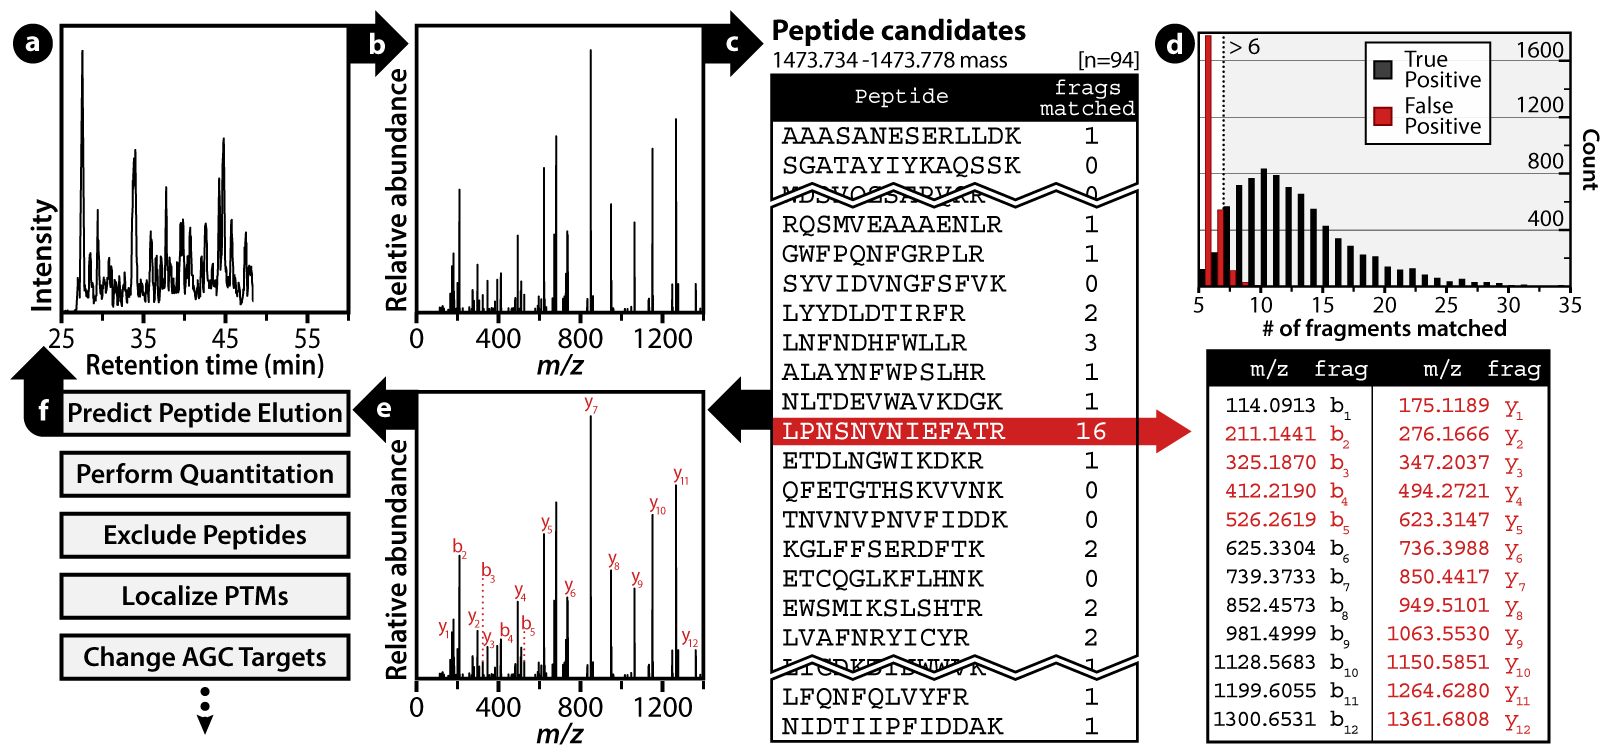
\includegraphics[width=\columnwidth]{inseq/inSeq_Fig 1.png}
	\mycaption{Progression of \inseq{} logic}{(A) A nHPLC-MS/MS chromatogram at 48.35 minutes along with an MS/MS scan (B) that was acquired at that time following dissociation of a +2 feature of \mz{} 737.86. Upon collection of the MS/MS scan, \inseq{} groups all peptide candidates (\emph{in silico}, n = 94) whose theoretical mass are within 30 ppm of the experimentally determined precursor neutral mass 1473.756 (C). Then \inseq{} performs \emph{in silico} fragmentation to produce a theoretical product ion series for each of the 94 candidates and proceeds to compare each to the experimental spectrum (<10 ppm mass accuracy). (D) Plot of \inseq{} identifications compared to conventional post-acquisition searching. \inseq{} agrees (True Positive) >98\% of the time when >6 fragment ions are matched.}
	\label{fig:inseq1}
\end{sidewaysfigure} 
The embedded peptide database-matching algorithm processes MS/MS scans immediately (Figure \ref{fig:inseq1}A\&B) by comparing product ions present in the MS/MS scan to those from peptide candidates pre-loaded onto the instrument's firmware. Note the candidate sequences are first filtered so that only sequences whose mass is within a small window (e.g., 5-50 ppm) of the sampled precursor neutral mass are considered (Figure \ref{fig:inseq1}C). For each candidate sequence the number of +1 product ions (+2 ions are included for precursors >+2) that matched the spectrum at a mass tolerance < 10 ppm is recorded (Figure \ref{fig:inseq1}C). Next, it uses straightforward scoring metrics, providing sufficient evidence for the confirmation of a putative sequence without burdening the system with non-essential calculations. On both MS platforms the real-time confirmation algorithm was expediently executed and required no hardware modification, taking an average of 16 ms to perform (Q Exactive, Figure \ref{fig:inseqs1}).
\begin{figure}[p]
	\centering
	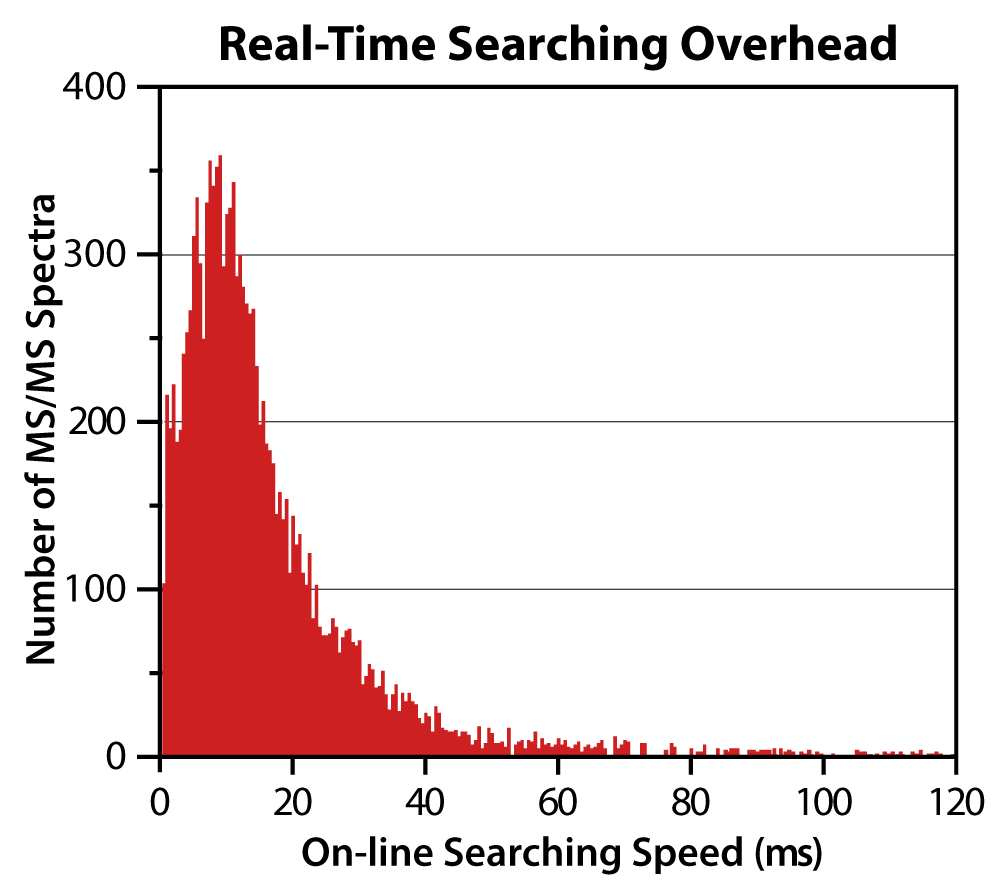
\includegraphics[width=\columnwidth]{inseq/inSeq_Fig S1.png}
	\mycaption{Distribution of \inseq{} analysis times (Q Exactive)}{The complete yeast proteome (6,717 proteins) was digested \emph{in silico}, trypsin specificity up to 3 missed cleavages) and the resulting peptides sorted to only retain those between 6-50 residues in length for a database of 1,174,780 unique sequences. The overhead accrued by \inseq{} is small ($\mu$ = 16 ms / spectrum) compared to the overall acquisition rate (\textasciitilde100-250 ms/spectrum), with over 95\% of the MS/MS events taking less than 45 ms to search.}
	\label{fig:inseqs1}
\end{figure}
To confirm that this small overhead does not affect the overall duty cycle, we compared the number of MS/MS scans performed when \inseq{} was and was not operating (9,076 DDA vs. 8,908 DDA with \inseq{}, \textasciitilde1.6\%). The number of MS scans for the peptide IVGIVSGELNNAAAK within its elution profile further demonstrates the negligible impact on duty cycle as 20 MS scans were taken with \inseq{} inactive as compared to 19 scans with \inseq{} active (Figure \ref{fig:inseqs2}).
\begin{figure}[p]
	\centering
	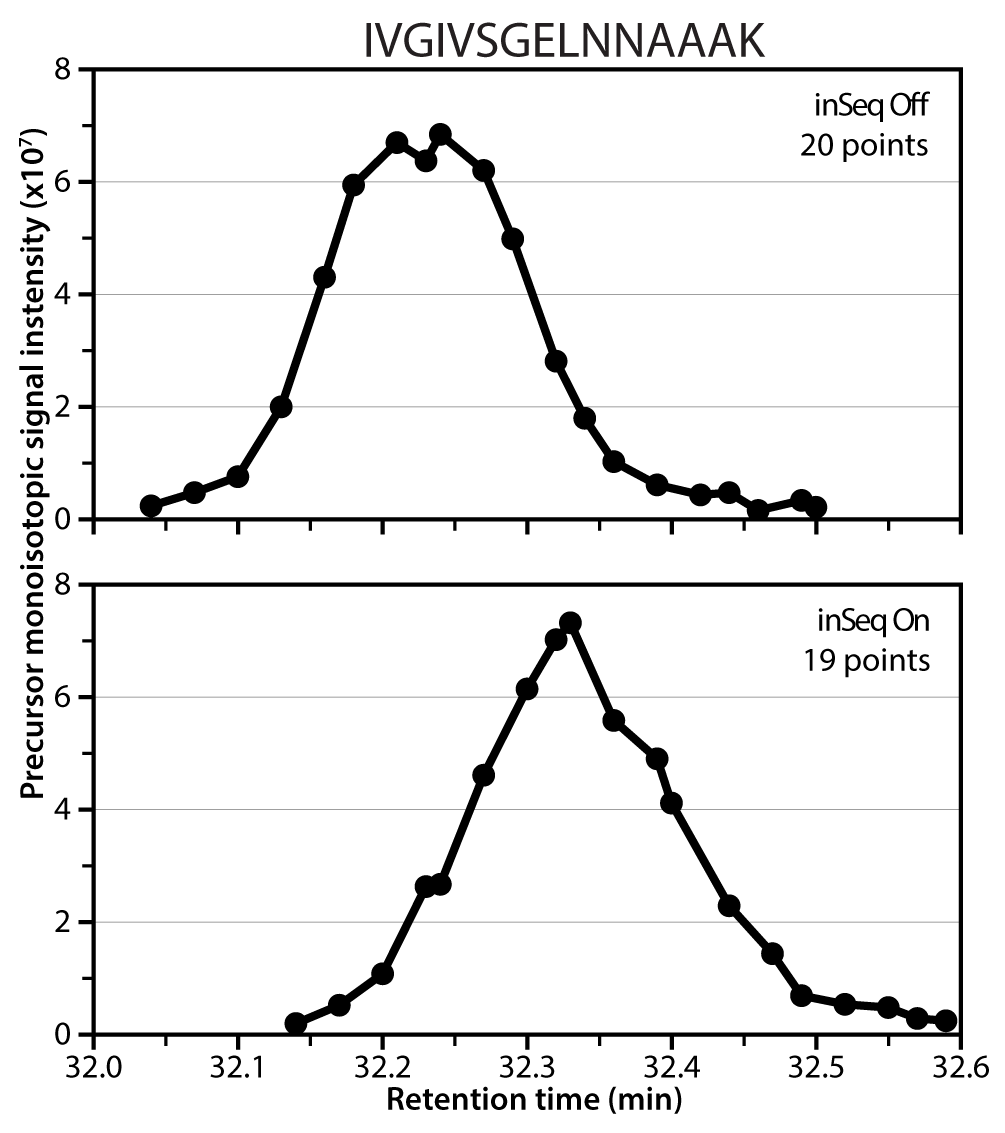
\includegraphics[width=\columnwidth]{inseq/inSeq_Fig S2.png}
	\mycaption{Frequency of MS scans with and without \inseq{} active}{The extracted ion chromatograms of a random peptide (IVGIVSGELNNAAAK) is displayed for two data-dependent top 10 experiments without (top) and with (bottom) \inseq{} active. In both cases, a large number of MS scans are performed within the elution profile (20 and 19 for \inseq{} off and on, respectively).}
	\label{fig:inseqs2}
\end{figure}

To characterize the \inseq{} algorithm we performed a nHPLC-MS/MS experiment on tryptic peptides derived from human embryonic stem cells. A database consisting of all theoretical tryptic peptides (up to three missed cleavages, 6-50 in length) contained within the human proteome was uploaded to the instrument's (Q Exactive) on-board computer. A DDA method was employed and analysis proceeded as usual, except following each MS/MS scan the \inseq{} algorithm was executed and the results logged. This manifest of instant identifications was then compared to those made post-acquisition via traditional database searching at a 1\% FDR (target-decoy method). We assumed the conventional post-acquisition approach to represent the true answer and compared the number of correct instant spectral identifications as a function of matched product ions (Figure \ref{fig:inseq1}D). From these data we conclude the detection of >6 product ions at high mass accuracy (<10 ppm) by the \inseq{} algorithm produces the correct sequence identification >98\% of the time. To determine the impact of \inseq{} on the depth of protein coverage, we compared OMSSA identifications with \inseq{} identifications (species with >6 matching peaks) (Figure \ref{fig:inseqs3}). Traditional post-acquisition searching identified more peptides than \inseq{} (11,095 vs. 7,910, respectively) indicating strong initial performance but also room for further development of a more sophisticated real-time scoring algorithm.
\begin{sidewaysfigure}[p]
	\centering
	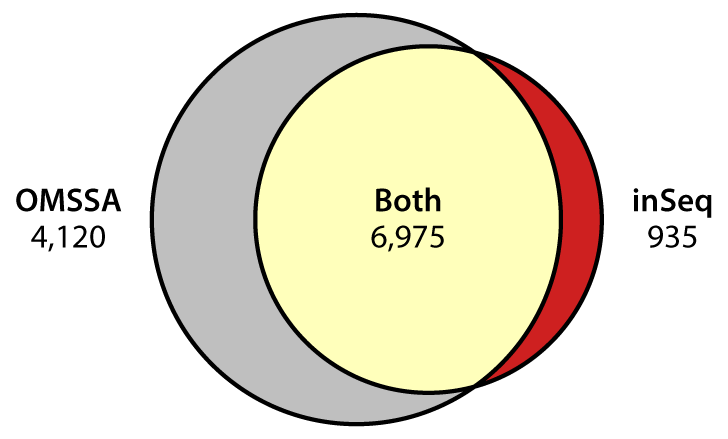
\includegraphics[width=\columnwidth]{inseq/inSeq_Fig S3.png}
	\mycaption{Overlap of \inseq{} and OMSSA identifications}{Each spectrum in a 120 min nHPLC-MS/MS gradient was scored with OMSSA and \inseq{}. OMSSA identifications were filtered to 1\% FDR and \inseq{} identifications were confirmed only if the spectra contained >6 matching peaks, as described in the text. Overlap between OMSSA and \inseq{} demonstrates that \inseq{} identifications are usually correct. The OMSSA-only identifications represent a subset of spectra which are false negatives with respect to \inseq{}.}
	\label{fig:inseqs3}
\end{sidewaysfigure}

\inseq{} represents a straightforward approach to correlate sequence to spectrum and is positioned to become an essential technology in transforming the current passive data collection paradigm. Specifically, learning the identity of a peptide that is presently eluting into the MS system permits an ensemble of advanced, automated decision-making logic. These concepts build upon our previous development of the data-dependent decision tree (DT) method. There we embedded an on-board algorithm to make unsupervised, real-time decisions of which fragmentation method to engage, based on precursor charge (\textit{z}) and \mz{}. Here, with the \inseq{} instant identification algorithm, we extend our simple DT method by adding several new decision nodes (Figure \ref{fig:inseqs4}). These nodes enable automated functionalities including: real-time elution prediction, advanced quantification, PTM localization, large-scale targeted proteomics, and increased proteome coverage, among others (Figure \ref{fig:inseq1}F).

\begin{figure}[p]
	\centering
	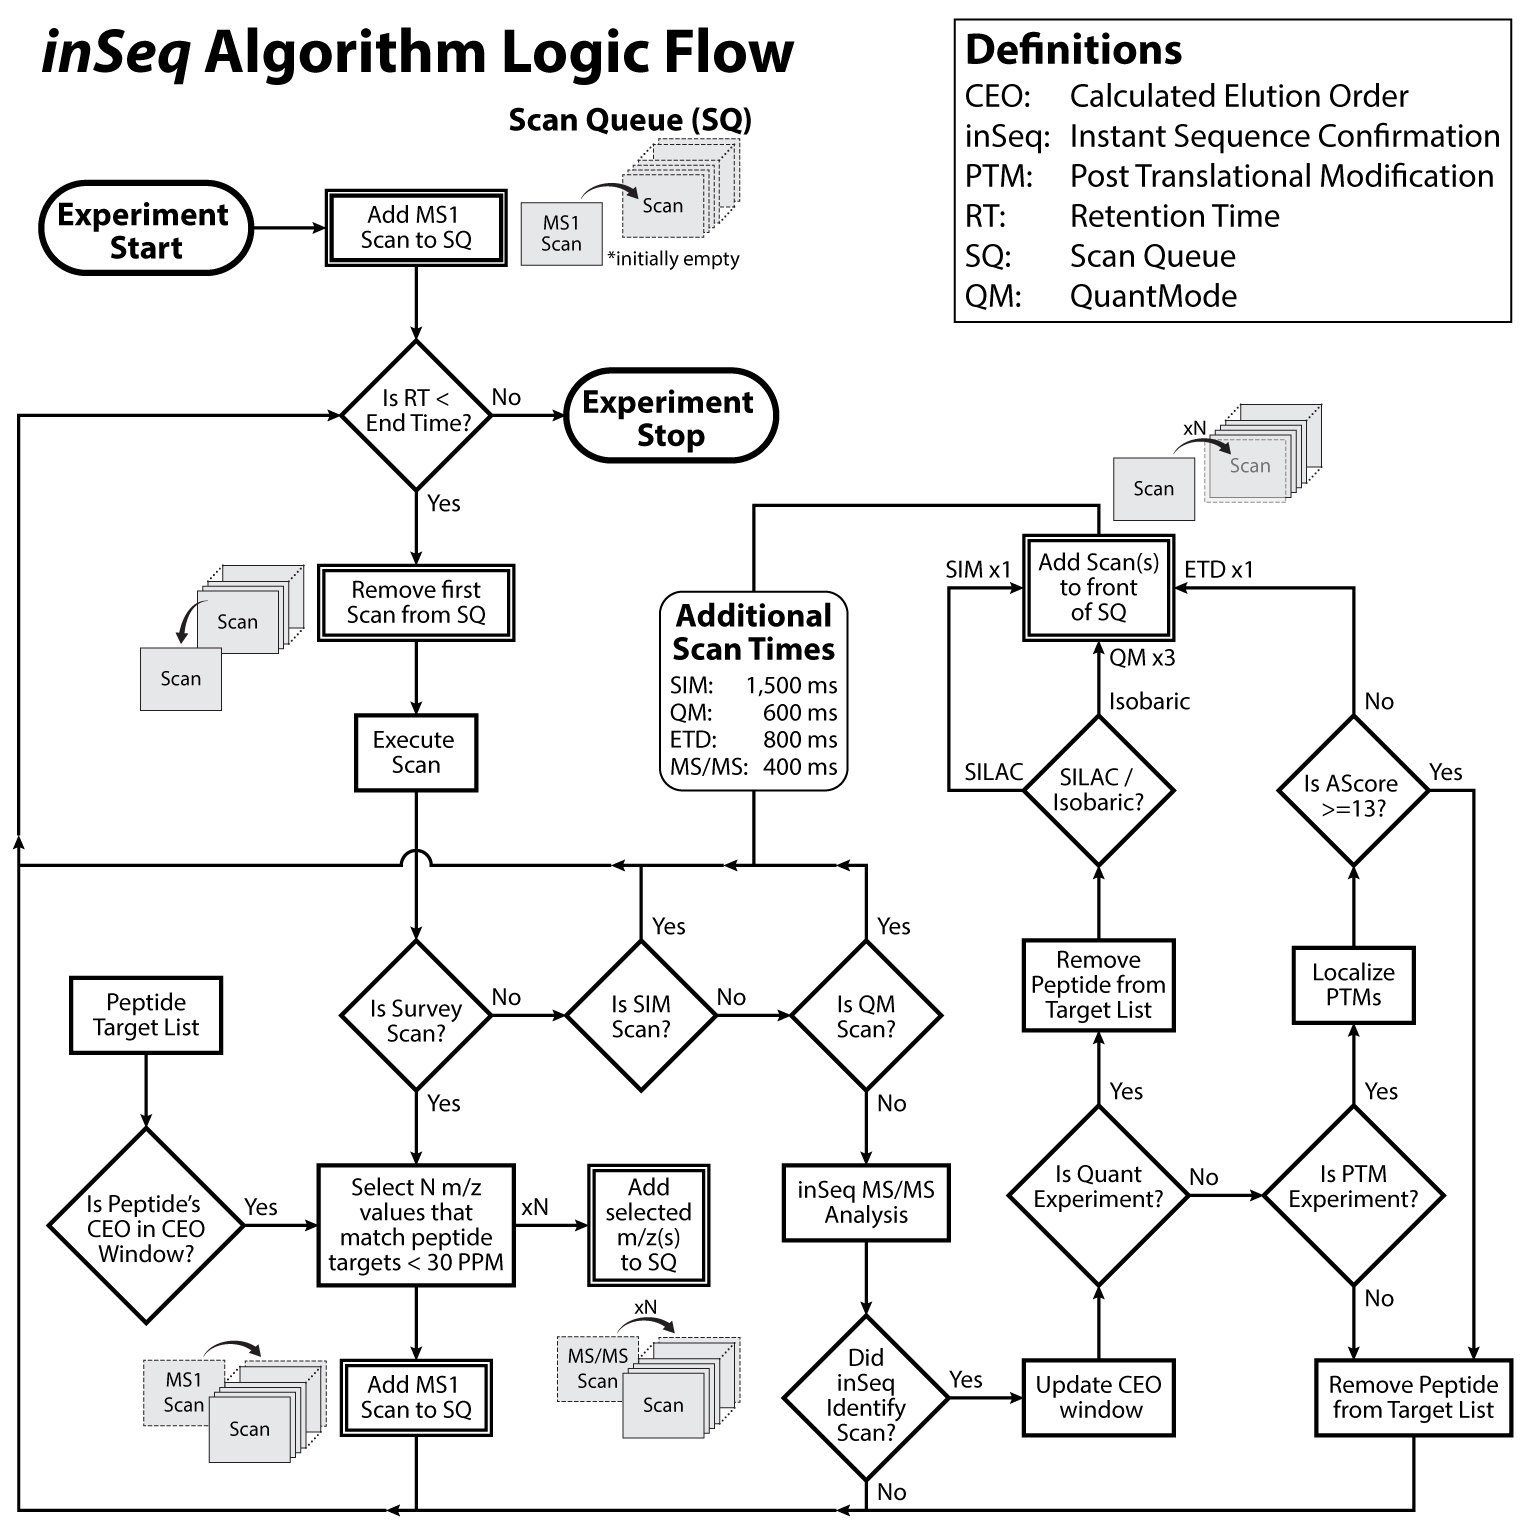
\includegraphics[width=\columnwidth]{inseq/inSeq_Fig S4.png}
	\mycaption{Basic information flow for implementing \inseq{}}{The flow of \inseq{} follows a targeted Top-N inclusion list (Target List) routine with additional analysis steps interspersed. Following an MS scan, the top 10 peaks that match precursors in the Target List (filtered by elution order) are added to a Scan Queue (SQ). Each MS/MS scan is analyzed with \inseq{} to determine if the peptide of interest is there. If identified, the peptide is removed from the Target List and additional analyses for quantitation and PTM localization may be performed.}
	\label{fig:inseqs4}
\end{figure}

\subsection*{Predicting peptide elution.}

Liquid chromatography is the conventional approach to fractionate highly complex peptide mixtures prior to measurement by MS. The highest MS sensitivity is achieved when one tunes the MS system to detect a given target (i.e., execute MS/MS) regardless of its presence in the preceding MS event (i.e., selected reaction monitoring). SRM measurements deliver both sensitivity and reproducibility at the cost of bandwidth. Specifically, if one does not know the elution time of a target, the duration of the nHPLC-MS/MS analysis must be dedicated to conditions for that specific entity. If elution times are known, then multiple SRM scan events can be programmed allowing for detection of multiple targets; however, chromatographic conditions must remain identical or the scheduled SRM elution windows will no longer align. Still, the bandwidth of that approach is low (\textasciitilde100 peptide targets per nHPLC-MS/MS analysis) and compiling such an experiment is highly laborious.\cite{indexion}

We surmised that \inseq{} could inform the MS system, without human intervention, of which peptide targets are most likely to subsequently elute. Such capability could enable robust, large-scale targeting (>500 per analysis) in an automated manner. Our approach relies upon relative peptide elution order and, consequently, bypasses the use of absolute retention times, which shift depending on chromatographic conditions and are not directly portable from multiple disparate experiments. Peptide elution order can be obtained in two ways: First, discovery experiments can be employed to determine retention order by normalizing the measured retention time for each detected peptide sequence. Second, the relative hydrophobicity for any sequence can be theoretically determined using existing software (e.g., SSRCalc).\cite{ssrcalc1,ssrcalc2,incselect} In our experience experimentally determined retention order offers better precision; still, it requires prior knowledge which may not be available. However retention order is determined, the real-time confirmation algorithm maintains a rolling average of the calculated elution order (CEO---a number describing the relative elution order of a target peptide) so that target peptides having nearby CEOs are specifically pursued (Figure \ref{fig:inseq1}B).
\begin{sidewaysfigure}[p]
	\centering
	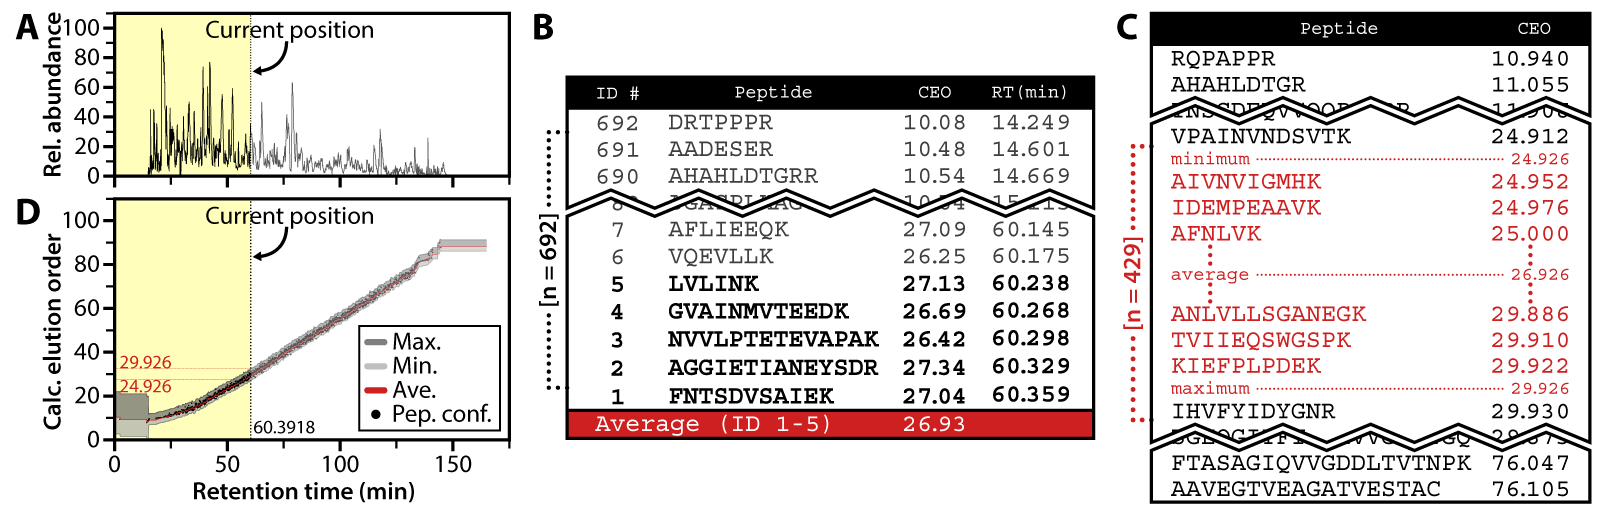
\includegraphics[width=\columnwidth]{inseq/inSeq_Fig 2.png}
	\mycaption{Elution order prediction using \inseq{}}{(A) Experimental chromatogram, 60.39 minutes into a 120 minute gradient, obtained while \inseq{} was recording instant identifications. (B) The \inseq{} calculated elution order (CEO) obtained by averaging the CEOs of the preceding 5 instantly identified peptides. (C) The asymmetric window (5 a.u.) surrounding the instant CEO average ($\mu$ = 26.926) and their corresponding sequences. (D) This analysis is repeated following each new peptide confirmation to constantly realign the CEO window based on current chromatographic conditions.}
	\label{fig:inseq2}
\end{sidewaysfigure}
Figure \ref{fig:inseq2} presents an overview of this approach. This example, 60.39 minutes into the chromatograph, highlights the last five \inseq{} identified peptides and their average CEO (26.926 a.u.). The on-board algorithm then computes an asymmetric CEO window (5 a.u., 24.926-29.926) that presents a short list of desired targets having CEOs within that range (Figure \ref{fig:inseq1}C). With this information the MS system can trigger specialized MS/MS scans specific to this refined target subset. Note that as targets are identified, the CEO window is dynamically adjusted so targets come into and out of the range precisely when they are eluting.

To test this technology, we performed a DDA nHPLC-MS/MS experiment in which tryptic peptides from a human ES cell sample were separated over a 60 minute gradient. Following data collection the resulting MS/MS spectra were mapped to sequence using database searching (1\% FDR). The unique peptide identifications (4,237) were sorted by observed retention time---this ordering then served as the CEO. 3,000 of these peptides were randomly selected as ''targets'' and loaded onto the instrument firmware (Velos-Orbitrap), along with their respective CEO, as a database for \inseq{}. The sample was then re-analyzed with \inseq{} activated, but with a doubled gradient length (120 min). Figure \ref{fig:inseq2}D displays the CEO window as calculated in real-time by the MS system (\inseq{}) plotted beside the actual elution time of identified peptides. Greater than 95\% of the peptides (2,889) fell within the rolling CEO window and were identified by both \inseq{} and post-acquisition searching. At our present capability we can achieve window widths similar to those used in absolute scheduling type experiments (\textasciitilde3-6 minutes) on a scale that is 30X larger (e.g., 3,000 targets vs. 100) with minimal effort.\cite{indexion,integrated} Further, we demonstrate that our approach adapts to different chromatographic conditions with no negative effects (Figure \ref{fig:inseq2}D). The key to the high portability and simplicity of our algorithm is the use of \inseq{} for continual, real-time realignment.

\subsection*{Improvement of quantitative accuracy.}

The method of stable isotope labeling has greatly propelled large-scale, quantitative analysis.\cite{pheromone,8plex,haploid,7tmr,esips,leeyeast} While generally robust, these techniques can yield spotty data for certain peptide and protein groups---mainly those present at low abundances. For SILAC, low signal-to-noise (S/N) precursor peaks in the MS scan often result in either omission of that particular feature or quantitative imprecision, if included.\cite{dynamicrange} For isobaric tagging, low intensity reporter ion signals (MS/MS) induce similar shortcomings.\cite{itraqerror} We surmised that \inseq{} could be employed to counter these limitations.

First, we developed an \inseq{} module to improve the quality of isobaric label-based measurements. The module analyzes MS/MS spectra, using \inseq{}, and, when a peptide of interest is detected, the quality of quantitative data is assessed. Should the reporter ion signals fall below a specified threshold, \inseq{} triggers follow-up scans to generate increased signal at the very instant the target peptide is eluting. In one implementation, we instructed \inseq{} to automatically trigger three quantitative scans, using the recently developed QuantMode (QM) method, to generate superior quality quantitative data on targets of high value.\cite{quantmode} The trio of QM scans are then summed offline.

To assess this decision node we analyzed a sample comprising three biological replicates of human embryonic stem cells pre- and two days-post bone morphogenetic protein 4 (BMP4) treatment (i.e., TMT 6-plex, three pre-treatment and three post BMP4 treatment cell populations). BMP4, a growth factor that induces context-dependent differentiation in pluripotent stem cells, is widely used to study differentiation to biologically relevant cell lineages such as mesoderm and endoderm.\cite{bmp,kdr,nanog} Whenever a target peptide was identified by \inseq{}, three QM scans were immediately executed. This ensured that all identified peptides had the same number of quantitation scans, enabling a direct comparison for analyzing multiple QM scans within this experiment.
\begin{sidewaysfigure}[p]
	\centering
	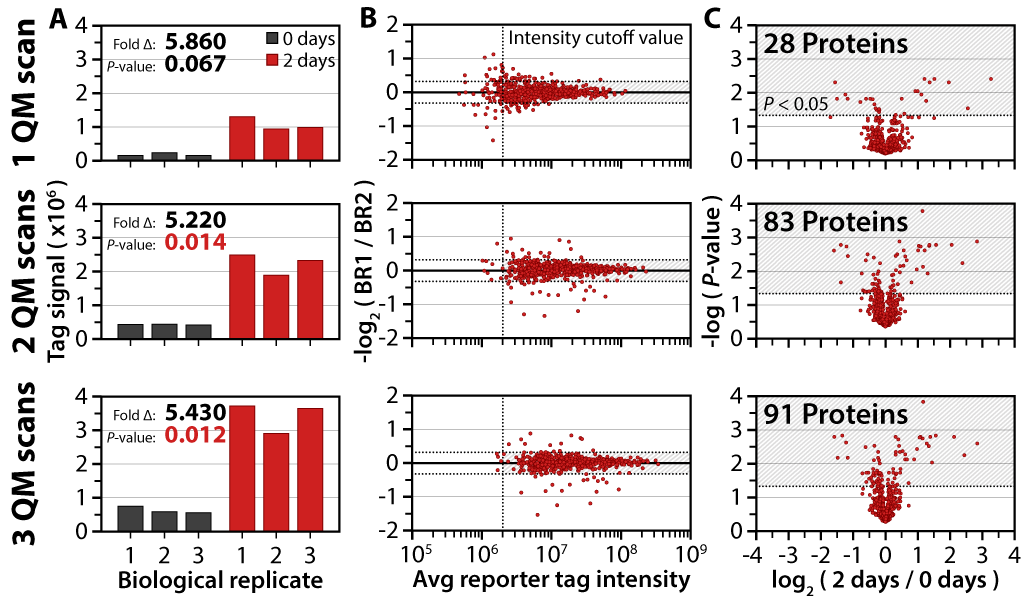
\includegraphics[width=\columnwidth]{inseq/inSeq_Fig 3.png}
	\mycaption{\inseq{} improves quantitative outcomes for isobaric tagging}{An \inseq{} decision node was written so that a real-time identification of a target sequence prompted automatic acquisition of three consecutive QuantMode (QM) scans. (A) Summing the reporter ion tag intensity from one, two, or three QM scans greatly improves the statistical significance of the measurement. (B) Summation of QM technical replicates reduces the variation in biological replicate measurement by increasing reporter ion S/N. (C) \inseq{}-triggered QM scans increase the number of significantly changing proteins from 28 to 91.}
	\label{fig:inseq3}
\end{sidewaysfigure}
Figure \ref{fig:inseq3}A demonstrates the benefit of summing isobaric tag intensities from one, two, or three consecutive quantitation scans for an \inseq{} identified target peptide having the sequence FCADHPFLFFIR from the protein SERPINB8. Here the ratio of change between control and treatment cell lines measured in one QM scan is large (5.86) but not significant (P = 0.067, Student's t-test with Storey correction).\cite{storey} Note significance testing was accomplished by assessing variation within the three biological replicates of both treatment and control cell lines. The measured ratio remains relatively unchanged (5.22 and 5.43) as reporter tag signals from additional quantitation scans are added; however, the corresponding P-values decrease to 0.014 and 0.012 when two or three quantitation scans are summed. By plotting the $\log_2$ ratio of quantified proteins from the three biological replicates against the average intensity of isobaric labels (Figure \ref{fig:inseq3} B) we demonstrate this improved significance results from boosted reporter S/N. Ideally this $\log_2$ ratio would be zero, indicating perfect biological replication; however, when only one quantitation scan is employed this ratio severely deviates from zero with decreasing tag intensity. To improve overall data quality and to omit potentially erroneous measurements we, and others, employ arbitrary reporter signal cutoffs (dashed vertical line in Figure \ref{fig:inseq3}B). Summation of additional quantitation scans increases the average reporter tag intensity, raising nearly all of the protein measurements above the intensity cutoff value (74, 9, and 4 proteins omitted using one, two, and three quantification scans, respectively). This quantification decision node also increased the number of proteins within 25\% of perfect biological replication (horizontal dashed line).

To determine if the method could improve the number of statistically significant differences between the cell populations, we calculated the $\log_2$ ratio of treated vs. control (i.e., 2 days/0 days) for each of the 596 quantified proteins (P<0.05, Student's t-test with Storey correction, Figure \ref{fig:inseq3}C). Only 28 proteins display significant change when one QM scan is used. By simply adding the reporter tag signal from additional scans the number of significantly changing proteins increases nearly threefold, from 28 to 91 when all three QM scans are analyzed together.
Many stable isotope incorporation techniques measure heavy and light peptide pairs in MS (e.g., SILAC). This approach, of course, requires the detection of both partners; note low abundance peptides are often identified with low, or no, precursor signal in the MS. We supposed that addition of another \inseq{} decision node could circumvent this problem. We cultured human embryonic stem cells in light and heavy media. Protein extract from these cultures was mixed 5:1 (light:heavy), before digestion overnight with LysC. The SILAC node was developed to select precursors from an MS scan only if the monoisotopic mass was within 30 ppm of any target on a list which contained 4,000 heavy and light peptides from a previous discovery run. Targets were selected only if the SILAC ratio deviated from the expected ratio of 5 by 25\%, i.e., the subset containing the most error. Following MS/MS, the resulting spectra were analyzed using \inseq{}. When a target of interest was identified, \inseq{} instructed the system to immediately record a SIM scan surrounding the light/heavy pair with a small, charge-dependent isolation window (\textasciitilde8-10 Th).

The average ratio of the light and heavy peptides subtly, but significantly, shifted from 4.47 under normal analysis to 5.34 for the \inseq{} triggered SIM scans (Student's t-test, p-value < 6\e{-20}). More importantly, the number of useable measurements, i.e., when both partners of the pair are observed, increased by \textasciitilde20\% (2,887 under normal analysis to 3,548 with \inseq{}, Figure \ref{fig:inseqs5}A).
\begin{sidewaysfigure}[p]
	\centering
	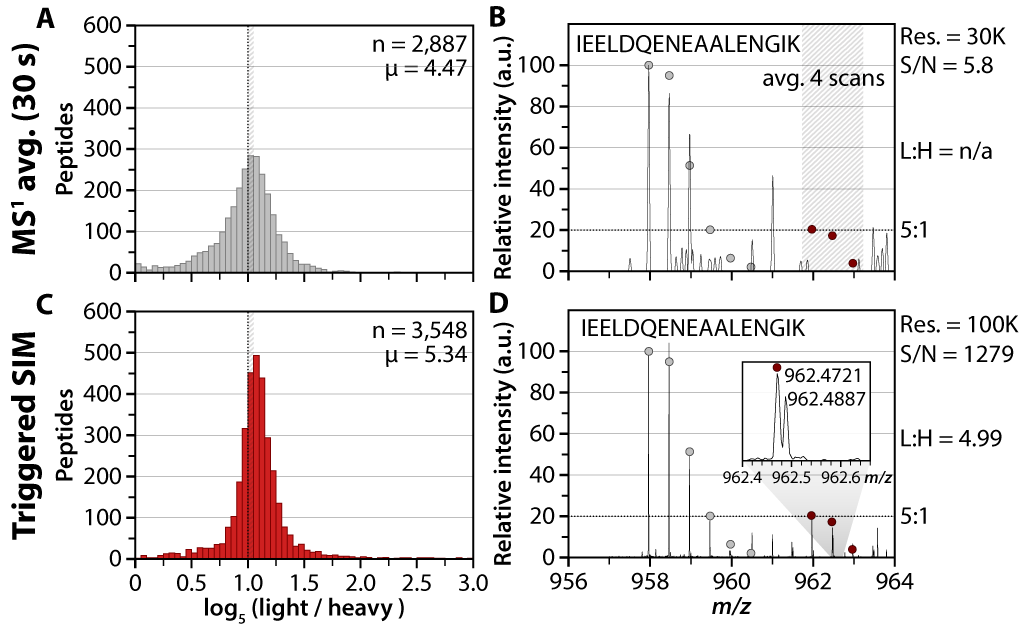
\includegraphics[width=\columnwidth]{inseq/inSeq_Fig S5.png}
	\mycaption{\inseq{} can improve quantitative outcomes for SILAC}{Following an \inseq{} confirmation of a peptide having the sequence, IEELDQENEAALENGIK, a narrow (8 Th), high-resolution (R = 100,000) SIM scan was automatically triggered and increased the S/N from 5.8 to 1,279 (Panels A and B). This SIM scan enabled detection of both partners and yielded the correct ratio of 5:1 (light:heavy). Besides increased dynamic range, the theoretical isotope distribution (shown in open circles) closely matches in the SIM scan (B), while the signal for the heavy partner is not even detectable in the MS (A). Over our entire data set, the \inseq{} triggered SIM scans improved the mean ratio from 4.47 to 5.34, but, more impressively, produced \textasciitilde20\% more quantifiable measurements (3,548 vs. 2,887).}
	\label{fig:inseqs5}
\end{sidewaysfigure}
Figure \ref{fig:inseqs5}B displays an example of the \inseq{}-triggered SIM scan and the increase in S/N and accuracy it affords. Here the MS/MS scan of the light partner was mapped, in real-time, to the sequence IEELDQENEAALENGIK. This event triggered a high resolution SIM scan (8 Th window), which led to the ratio of 4.99:1 (correct ratio 5:1). Here gas phase enrichment was essential to quantify the relative abundance, as the isotopic envelope of the heavy partner was not observed, even with extensive spectral averaging of successive MS scans (\textasciitilde30 s, Figure \ref{fig:inseqs5}B). Whether for MS or MS/MS centric methods, we conclude that \inseq{} technology will significantly improve the quality of quantitative data with only a minimal impact on duty cycle.

\subsection*{Post-Translational Modification Site Localization.}

The presence of post-translational modifications (PTMs) on proteins plays a major role in cellular function and signaling. Unambiguous localization of PTMs to residue demands observation of product ions resulting from cleavage of the residues adjacent to the site of modification, i.e., site-determining fragments (SDFs). In a typical analysis only about half of the identified phosphorylation sites can be mapped with single amino acid resolution, stymying systems-level data analysis. We reasoned that \inseq{} could be leveraged to boost PTM localization rates by dynamically modifying MS/MS acquisition conditions when necessary. As such we developed an online PTM localization decision node to determine, within milliseconds, whether a MS/MS spectrum contains SDFs to unambiguously localize the PTM. Should SDFs be lacking, \inseq{} instantly orchestrates further interrogation.

The PTM localization node is engaged when \inseq{} confirms the detection of a PTM-bearing peptide. After the sequence is confirmed, \inseq{} assesses the confidence with which the PTM(s) can be localized to a particular amino acid residue. This procedure is accomplished by computing an online probability score similar to post-acquisition PTM localization software---i.e., AScore.\cite{ascore} Briefly, \inseq{} compares all possible peptide isoforms against the MS/MS spectrum. For each SDF the number of matches at <10 ppm tolerance is counted and an AScore is calculated (\inseq{} uses similar math). If the AScore of the best fitting isoform is above 13 (p < 0.05) the PTM is declared localized. When the AScore is below 13, however, \inseq{} triggers further characterization of the eluting precursor until either the site has been deemed localized or all decision nodes have been exhausted. Additional characterization can include many procedures such as acquisition of MS/MS spectra using different fragmentation methods (e.g., CAD, HCD, ETD, PD, etc.), varied fragmentation conditions (e.g., collision energy, reaction time, laser fluence, etc.), increased spectral averaging, MSn, pseudo MSn, modified dynamic exclusion, and altered AGC target values, among others.\cite{neutralloss}
\begin{figure}[p]
	\centering
	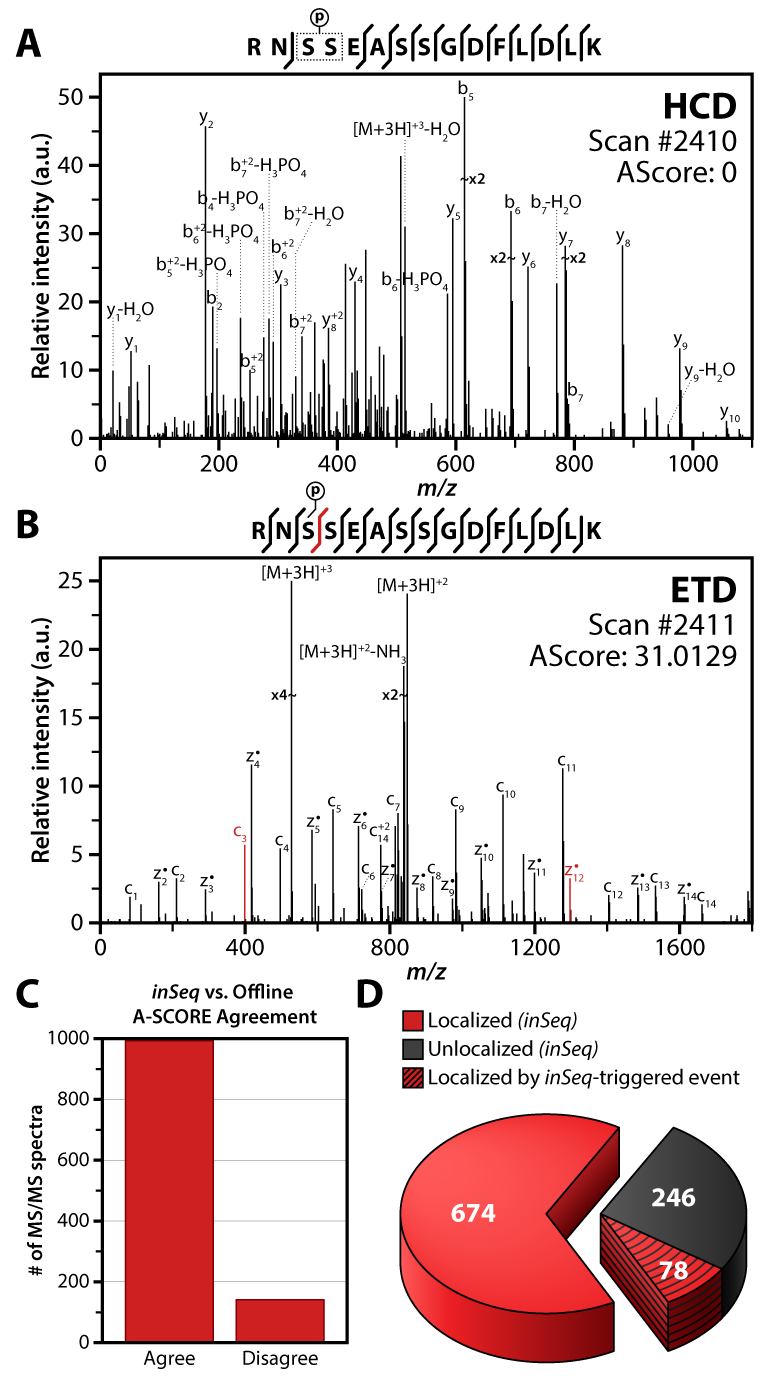
\includegraphics[width=0.6\columnwidth]{inseq/inSeq_Fig 4.png}
	\mycaption{\inseq{} can improve PTM localization rates}{Following MS/MS (HCD) of the singly-phosphorylated precursor RNsSEASSGDFLDLK, \inseq{} could not find sufficient information to confidently localize the modification to either Ser 3 or 4 (A, AScore = 0). \inseq{} immediately triggered an ETD MS/MS scan event on the same precursor (B). This spectrum was assigned an AScore of 31.0129 (phosphorylation on Ser3) and was considered confidently localized---note the SDFs $c_3$ and $z\cdot_{12}$ ions. (C) Globally, the \inseq{} localization calculation agreed with offline analysis using the actual AScore algorithm. (D) Using a simple dissociation method DT, \inseq{} produced a confidently localized phosphorylation site for 78 of 324 unlocalizable sites, saving nearly 25\% of them.}
	\label{fig:inseq4}
\end{figure}

To obtain proof-of-concept results we wrote a simple \inseq{} node that triggered an ETD MS/MS scan of phosphopeptides that were not localized following HCD MS/MS. In one example (Figure \ref{fig:inseq4}) the sequence, RNSSEASSGDFLDLK, was confirmed to contain a phosphoryl group; however, the \inseq{} algorithm could not confidently localize the PTM to any of the four Ser residues (AScore = 0). Next, \inseq{} triggered an ETD MS/MS scan of the same precursor (Figure \ref{fig:inseq4}B). The resulting spectrum was then analyzed for the presence of the SDFs, \fragment{c}{3} / \fragment{z\cdot}{12}. Both of these fragments were present and the site was localized to Ser 3 with an AScore of 31.0129 (p < 0.00079). Post-acquisition analysis confirmed the results of our online \inseq{} approach---both spectra (HCD and ETD) were confidently identified and their calculated AScores were 0 and 45.58, respectively. When compared on a global scale, 993 of the 1,134 \inseq{}-identified phosphopeptides had localization judgments that matched post-acquisition AScore analysis (Figure \ref{fig:inseq4}). This slight difference is the result of using different localization algorithms for online and post-acquisition analysis. Primarily, the post-acquisition method considers fragment ions on either side of the site-determining fragments separately, while the \inseq{} method does perform this extra step for simplicity.\cite{esips,ascore} These data demonstrate that our localization node is highly effective at instantaneously determining whether a PTM site can be localized. Unfortunately, only marginal gains were achieved in this basic implementation as most precursors were doubly charged and, therefore, not effectively sequenced by ETD. Next, we modified the \inseq{} decision node to incorporate a dissociation method DT. Here a follow-up ETD or combination ion trap CAD/HCD scan was triggered depending upon precursor charge (\textit{z}) and \mz{}. With the slightly evolved algorithm the \inseq{} method detected 998 phosphopeptides in a single shotgun experiment. It determined that 324 of these identifications lacked the information to localize the PTM site and, in those cases, triggered the new dissociation decision node. 78 of these unlocalizable sites were confidently mapped with this technique---salvaging nearly 25\% of the unlocalized sites (Figure \ref{fig:inseq4}D). These encouraging results demonstrate that \inseq{} has great promise to curtail the problem of PTM localization in a highly automated fashion. We note there are dozens of parameters to explore in the continued advancement of this PTM localization decision node.

\section{Conclusion}

Here we described an instant sequencing algorithm (\inseq{}) that operates using the pre-existing processors of the MS. Rapid real-time sequencing affords several novel data acquisition opportunities. To orchestrate these opportunities we constructed an advanced decision tree logic that extends our earlier use of the method to intelligently select dissociation type. The approach can circumvent longstanding problems with the conventional DDA paradigm. We provided three such examples herein. First, we demonstrated that knowledge of which peptide sequences are eluting can facilitate the prediction of soon to elute targets. This method shows strong promise to revolutionize the way in which targeted proteomics is conducted. Second, we used quantitative decision nodes that fired when \inseq{} detected a peptide sequence of interest. With either SILAC or isobaric tagging, significant gains in quantitative outcomes were documented. Third, we endowed \inseq{} with an instant PTM site-localization algorithm to determine whether or not to initiate more rigorous follow-up at the very instant the peptide of interest was eluting. We show that the \inseq{} site localizer is highly effective (90\% agreement with post-acquisition analysis) and that triggering a simple dissociation method DT can improve site localization by \textasciitilde25\%. Further development will doubtless deliver additional gains.

Targeted proteomics is an area of increasing importance. Following discovery analysis it is natural to cull the list of several thousand detected proteins to several hundred key players. In an ideal world these key proteins are then monitored in dozens or even hundreds of samples with high sensitivity and reproducibility, without rigorous method development and be expediently performed. We envision that advanced DT analysis with \inseq{} could offer such a platform. Using the retention time prediction algorithm we introduced here one can foresee the \inseq{} algorithm quickly and precisely monitoring hundreds of peptides without the extensive labor and pre-planning required by the selected reaction monitoring (SRM) technique, current state-of-the-art.\cite{srm} Other possibilities include automated pathway analysis where user-defined proteins, within a collection of pathways, are simply uploaded to the MS system. Then, \inseq{} automatically determines the best peptides to track, their retention times, and constructs the method. Two key advantages over current SRM technology make this operation possible. First, knowledge of specific fragmentation transitions are not necessary as all products are monitored with high mass accuracy. Second, precise elution time scheduling is not necessary as \inseq{} can use CEO, experimental or theoretical, to dynamically adjust the predicted elution of targets. In this fashion the most tedious components of the SRM workflow can be avoided.

\section{Experimental Methods}

\subsection{Cell Culture.}
Human embryonic stem cells (line H1) were maintained in feeder independent media as previously described.\cite{feeder} For SILAC experiments, DMEM/F12 lacking lysine and arginine (Mediatech Inc.) was supplemented with light arginine (Sigma-Alrich) and either heavy labeled lysine (Cambridge Isotopes Laboratories) or light lysine (Sigma-Aldrich). Cells were cultured on Matrigel (BD Biosciences) and split 1:8 at approximately 80\% confluency using 0.1 mM EDTA. To harvest cells, TripLE Express (Invitrogen) was applied for five minutes at 37$^\circ$C. Following cell detachment, an equivalent volume of ice-cold DPBS (Invitrogen) was added before centrifugation. Cell pellets were subsequently washed twice in ice-cold DPBS and stored at $-80^\circ$C. BMP4-treated cells were grown and harvested as described above, except that 5 ng/mL BMP4 (R\&D Systems) was added into the media and cells were split using TrypLE (Invitrogen). For BMP4 experiments, single cells were plated at the density of 4\e{4}/cm$^2$, for 2 days of treatment. We collected \textasciitilde$10^8$ cells for each analysis.

\subsection{Cell Lysis.}
For all analysis, human embryonic stem cells were lysed in ice-cold 8 M urea, 40 mM NaCl, 50 mM tris (pH 8), 2 mM MgCl$_2$, 50 mM NaF, 50 mM $\beta$-glycerol phosphate, 1 mM sodium orthovanadate, 10 mM sodium pyrophosphate, 1X mini EDTA-free protease inhibitor (Roche Diagnostics), and 1X phosSTOP phosphatase inhibitor (Roche Diagnostics). To solubilize protein and ensure complete lysis, samples were sonicated three times for 15 seconds with 30 second pauses. Total protein was then quantified using a BCA protein assay kit (Thermo Scientific Pierce).

\subsection{Isobaric Label Sample Preparation.}
For analysis, 250 $\mu$g of protein from each sample was reduced by adding DTT to a final concentration of 5 mM, and alkylated with 15 mM iodoacetamide before final capping with 5 mM DTT. Digestion was carried out by adding LysC (Wako Chemicals) at a 1:100 enzyme-to-protein ratio and incubating at 37$^\circ$C for 2 hours. At this time, the lysate was diluted with 25 mM tris (pH 8) to a final urea concentration of 1.5 M and further digested for 12 hours at 37$^\circ$C with trypsin (Promega) at a 1:100 enzyme to protein ratio. Peptides were then acidified with TFA to quench the reaction and de-salted using C-18 solid phase extraction (SPE) columns (Waters). TMT labeling was carried out per manufacturer's directions (Thermo Scientific Pierce). Samples were mixed in a 1:1:1:1:1:1 ratio before analysis.

\subsection{SILAC Sample Preparation.}
Protein from the light and heavy embryonic stem cell cultures was mixed in a 5:1 ratio (light:heavy) by pooling 2.5 mg of light protein and 0.5 mg of heavy protein. The sample was reduced by adding DTT to a final concentration of 5 mM, and alkylated with 15 mM iodoacetamide before final capping with 5 mM DTT. Digestion was carried out by adding LysC (Wako Chemicals) at a 1:100 enzyme-to-protein ratio and incubating at 37$^\circ$C overnight. Peptides were then acidified with TFA to quench the reaction and de-salted using C-18 solid phase extraction (SPE) columns (Waters).

\subsection{Phosphopeptide Sample Preparation.}
From an embryonic stem cell culture, 1 mg of protein was reduced by adding DTT to a final concentration of 5 mM, and alkylated with 15 mM iodoacetamide before final capping with 5 mM DTT. Digestion was carried out by adding LysC (Wako Chemicals) at a 1:100 enzyme-to-protein ratio and incubating at 37$^\circ$C for 2 hours. At this time, the lysate was diluted with 25 mM tris (pH 8) to a final urea concentration of 1.5 M and further digested for 12 hours at 37$^\circ$C with trypsin (Promega) at a 1:100 enzyme to protein ratio. Peptides were then acidified with TFA to quench the reaction and de-salted using C-18 solid phase extraction (SPE) columns (Waters).
Phosphopeptides were enriched via immobilized metal affinity chromatography (IMAC) using magnetic beads (Qiagen). Following equilibration with water, the beads were treated with 40 mM EDTA (pH 8.0) for 30 minutes with shaking, and washed 3X with water again. The beads were then incubated with 100 mM FeCl$_3$ for 30 minutes with shaking and finally were washed 3 times with 80\% acetonitrile/0.1\% TFA. Samples were likewise resuspended in 8\% acetonitrile/0.15\% TFA and incubated with beads for 45 minutes with shaking. The resultant mixture was washed 3 times with 1 mL 80\% acetonitrile/0.1\% TFA, and eluted using 1:1 acetonitrile:0.7\% NH$_4$OH in water. Eluted phosphopeptides were acidified immediately with 4\% formic acid and lyophilized to \textasciitilde5 $\mu$L.

\subsection{nano-High Performance Liquid Chromatography.}
For all samples online reverse-phase chromatography was performed using a nanoACQUITY UPLC system (Waters). Peptides were loaded onto a pre-column (75 $\mu$m ID, packed with 7 cm C18 particles, Alltech) for 10 min at a flow rate of 1 $\mu$L/min. Samples were then eluted over an analytical column (50 $\mu$m ID, packed with 15 cm C18 particles, Alltech) using either a 60 or 120 min linear gradient from 2\% to 35\% acetonitrile with 0.2\% formic acid and a flow rate of 300 nL/min.

\subsection{Target List Construction and \inseq{} Setup.}
For all experiments, the monoisotopic mass, charge state, and previously determined retention time of target peptides was included for use by the \inseq{} algorithm. In addition, peptides modified on methionines or tyrosines were omitted from all target lists. For peptide elution and isobaric label quantitation \inseq{} experiments, a target list of 4,000 peptides was constructed from a previous nHPLC-MS/MS experiment employing a 90 min nHPLC gradient. For SILAC \inseq{} experiments, peptides identified at 1\% FDR in a discovery nHPLC-MS/MS experiment were analyzed to determine the light:heavy partner ratio. A target list of 2,000 peptide pairs (4,000 total peptides) whose ratio deviated from the expected value of 5 by at least 25\% was constructed. This subset of peptides included many measurements in which the signal to noise was low, or a partner was missing. For phosphorylation \inseq{} experiments, phosphopeptides identified at 1\% FDR in a discovery nHPLC-MS/MS experiment were analyzed by the Phosphinator localization software to assign phosphosite locations. A target list comprising 2,174 phosphopeptides was constructed and used for both ETD only and decision tree (DT) \inseq{} methods.

Target lists were loaded into the instrument's firmware for instant access during acquisition. Peptide lists were stored in an internal database and sorted based on their precursor mass for fast look ups using a binary search algorithm. A parameter file was preloaded into the firmware prior to each experiment to specific scan sequences and instrument parameters needed for the intended experiment.

\subsection{Mass Spectrometry.}
All experiments were performed on Thermo LTQ Orbitrap Velos and Q Exactive mass spectrometers. The LTQ Orbitrap Velos used firmware version 2.6.0.1065 SP3 with additional ion trap control language (ITCL) modifications to enable \inseq{} operation. MS scans were performed in the Orbitrap at 30,000 resolution at a max injection time of 500 ms and a target value of 1e6. MS/MS scans were also performed in the Orbitrap at a resolution of 7,500 and with HCD normalize collision energy (NCE) of 27\%, for a max fill time of 500 ms. The Q Exactive was operated using version 2.0 Build 142800 with a modified python code base for \inseq{} data acquisition control. Q Exactive MS scans were collected at 70,000 resolution for a max injection time of 120 ms or if the 1e6 AGC target value was reached. MS/MS events were measured at 17,500 resolution at a target value of 1e5, 120 ms max injection time and 26\% NCE. Instrument methods for both the LTQ Orbitrap Velos and Q Exactive were overridden during acquisition by the instrument's firmware to provide for dynamic \inseq{} operation. Processing times for \inseq{} were similar on the older Velos-Orbitrap system with the newer Q Exactive; however, a \textasciitilde100 ms overhead was included because complete collection of the Orbitrap transient signal is necessary before the spectrum can be examined.

\subsection{Database searching and FDR estimation.}
MS/MS data was analyzed using the Coon OMSSA Proteomics Software Suite (COMPASS).\cite{compass} The Open Mass Spectrometry Search Algorithm (OMSSA; version 2.1.8) was used to search spectra against the International Protein Index(IPI) human database version 3.85.\cite{omssa} For all experiments, carbamidomethylation of cysteines was included as a fixed modification, while oxidation of methionines was set as a variable modification. For TMT experiments, TMT on the N-terminus and TMT on lysines were included as fixed modifications and TMT on tyrosines was added as a variable modification. For SILAC experiments heavy lysine was added as a variable modification. Precursor mass tolerance was set to $\pm$4.5 Da and monoisotopic mass tolerance was set to $\pm$0.015 Da for fragment ions. Results were filtered to a 1\% FDR at both the peptide and protein level with a maximum precursor mass error of 50 ppm. For phosphopeptides, the Phosphinator software was used to localize phosphorylation sites.\cite{esips}

\subsection{Protein and Peptide Quantification.}
TMT quantification was performed using TagQuant within COMPASS. This program extracts reporter ion intensities and multiplies them by injection times to determine counts. Purity correction was performed as previously described.\cite{itracker} Tag intensities were normalized to ensure that the total signal from each channel was equal. For evaluation of multiple QuantMode (QM) scans, data was analyzed at the peptide level by only quantifying the first, the sum of first and second, or the sum of the first, second, and third QM scans using TagQuant. Peptides were then combined into protein groups (ProteinHerder) and quantified at the protein level (ProteinTagQuant) within COMPASS. Experimental ratios and p-values (Student's t-test assuming equal variance) were determined using Microsoft Excel. To correct for multiple hypothesis testing, we applied Storey correction using the freely available program QVALUE.\cite{storey}
SILAC quantification was performed with in-house software that retrieved the peak intensities of both SILAC partners from either a single \inseq{}-triggered SIM scan (monoisotopic peak) or performed an extracted ion chromatogram (30 sec window) of identified precursor. A ratio of partner abundance was only calculated if both SILAC partners had an intensity at least twice that of the noise.

\bibliographystyle{ieeetr}
\bibliography{inseq}


\chapter{Intelligent data acquisition blends targeted and discovery methods.}

\section{Summary}

A MS method is described here that can reproducibly identify hundreds of peptides across multiple experiments. The method uses intelligent data acquisition (IDA) to precisely target peptides while simultaneously identifying thousands of other, non-targeted peptides in a single nano-LC-MS/MS experiment. We introduce an online peptide elution order alignment (EOA) algorithm that targets peptides based on their relative elution order, eliminating the need for retention time-based scheduling. We have applied this method to target 500 mouse peptides across six technical replicate nano-LC-MS/MS experiments and were able to identify 440 of these in all six, compared to only 201 peptides using data-dependent acquisition (DDA). A total of 3,757 other peptides were also identified within the same experiment, illustrating that this hybrid method does not eliminate the novel discovery advantages of DDA. The method was also tested on a set of mice in biological quadruplicate and increased the number of identified target peptides in all four mice by over 80\% (826 vs. 459) compared with the standard DDA method. We envision real-time data analysis as a powerful tool to improve the quality and reproducibility of proteomic datasets.

\section{Introduction}

Large-scale proteomic studies make use of a variety of tools and techniques to achieve depth and wide coverage of proteomes. The most popular method for sequencing proteomes is shotgun sequencing where peptides are digested from extracted proteins, separated with chromatography (HPLC), and then mass analyzed using mass spectrometry (MS).\cite{mudpit,mudpit2} Since complex proteomes can encompass thousands of proteins, leading to millions of peptides, deciding how to allocate the limited mass spectrometer bandwidth is key to successful analysis.\cite{100000} By far the most successful method for this time management is data dependent acquisition (DDA), where intact peptide precursors are first mass analyzed (MS1), specific \mz{} features are then selected to undergo fragmentation, and finally the fragment ions are mass analyzed again (MS/MS). This process is repeated throughout the LC separation, resulting in a large collection of MS and MS/MS spectra. Peptides are eventually identified from the fragmentation spectra and then grouped together back into their parent proteins.\cite{sequest,sadygov,venable,panda} This approach has produced outstanding results in the past decade, but, due to variety of reasons (e.g., large protein dynamic range, speed of MS instrumentation, separation efficiency, etc.) undersampling of proteomes is very common. In other words, not every peptide is identified in every LC-MS/MS experiment. Incomplete datasets limit the questions researchers can answer, especially when biological replication is used to increase statistical power, many measurements become worthless if they cannot be measured reproducibly.\cite{quant} As proteomics seeks to answer global biological questions, reproducible peptide identification between datasets is mandated.\cite{ideker,msbp,molloy}

Many studies have outlined the problem of poor peptide reproducibility.\cite{liu,mrm,tabb,bigtime,pachl} Aebersold succinctly summarized that irreproducibility is a multifaceted issue, depending on user experience, equipment, and data analysis, among others.\cite{aebersold} He outlines that there are two main approaches in tackling irreproducibility. First, exhaustively identify every peptide in a sample -- an approach that is becoming more feasible as technology improves.\cite{thakur,nagaraj,onehour} The more common approach, as many other researchers have embarked on, is to focus on a smaller subset of peptides and to thoroughly identify and quantify those using targeted methods.\cite{savitski} Methods such as selected reaction monitoring (SRM) are powerful and reproducible, but are low throughput, targeting a few hundred peptides at most.\cite{lange,picotti1,picotti2} To improve identification reproducibility and throughput, targeted methods almost exclusively rely on retention time-based scheduling, segmenting the MS duty cycle among the target peptides. In SRM methods, a series of MS/MS transitions for each targeted peptide is automatically collected at the appropriate retention time (RT), removing the dependence on MS1 detection. This requires precise knowledge of the peptide retention time for the LC-MS system and is low throughput as only one set of transitions are monitored at a given point in time. Recent work on intelligent SRM (iSRM) increases throughput by monitoring only a subset of transitions for each target, switching to normal SRM when these transitions are detected.\cite{isrm} We sought to expand upon the idea of intelligent real-time switching of methods by combining the enhanced reproducibility of targeted scheduled methods with the novel discovery advantages of DDA in a single hybrid method. Our goals were three-fold: first, to develop a method that increases the throughput of targeting; second, to replace retention-time based scheduling and its laborious method development with a more robust and straightforward peptide elution ordering; and last, to maintain the discovery aspect of DDA sampling while simultaneously targeting a subset of peptides.

In the last decade, a few computational approaches have been aimed at solving the problem of poor reproducibility. The concept of accurate mass tags (AMT) was first introduced by Smith et. al. as a means to identify peptides in multiple runs based on accurate mass and retention time.\cite{smith} This concept was further expanded with PepMiner and PEPPeR, tools for clustering features among multiple datasets.\cite{pepminer,pepper} Most notably, Prakash et. al. introduce the concept of aligning multiple MS datasets based on peptide relative elution order into signal maps.\cite{prakash} To date, these and other computational methods\cite{radulovic,listgarten,shen,zhang,lin,bateman} have been performed post-acquisition, attempting to improve already collected data. We seek to improve the reproducibility at the source by improving the algorithms the MS uses to select precursors to fragment. We and others have proposed using real-time data analysis and dynamic MS control as a means for improving the quality of acquired spectra.\cite{inseq,graumann,webber} Here we present our findings on combining accurate mass, elution orders, and real-time data analysis to improve the sampling reproducibility of the MS.

\section{Results and discussion}

\subsection*{Irreproducible Peptide Identification.}
In data dependent acquisition (DDA) peptide precursors are selected for fragmentation based on intensity in a MS1 survey scan. This straightforward approach has proven to be a simple and powerful technique. However, it is pestered with inconsistent sampling, and therefore, irregular peptide identification between experiments. The DDA method is inherently stochastic in nature, depending heavily on the consistency of the input data (MS1) to deliver reproducible peptide identification (MS/MS). Even the slightest change in the chromatography or ionization efficiencies will have repercussions on the collection of the whole dataset (e.g., the butterfly effect). To characterize the extent these minor changes have on the reproducibility of peptide identifications, six replicate injections of a tryptic digest of yeast whole cell lysate were analyzed using DDA on the same nano-LC-MS/MS system over a span of ten days. On average, each experiment identified 13,289 $\pm$ 340 unique peptide sequences (I/L ambiguity removed) at a 1\% FDR, indicating a highly consistent separation and nearly identical instrument performance. Of the 23,919 unique peptides identified in total, only 5,404 (22.6\%) of those peptide were identified in all six experiments (Figure \ref{fig:eoa1}).
\begin{sidewaysfigure}[p]
	\centering
	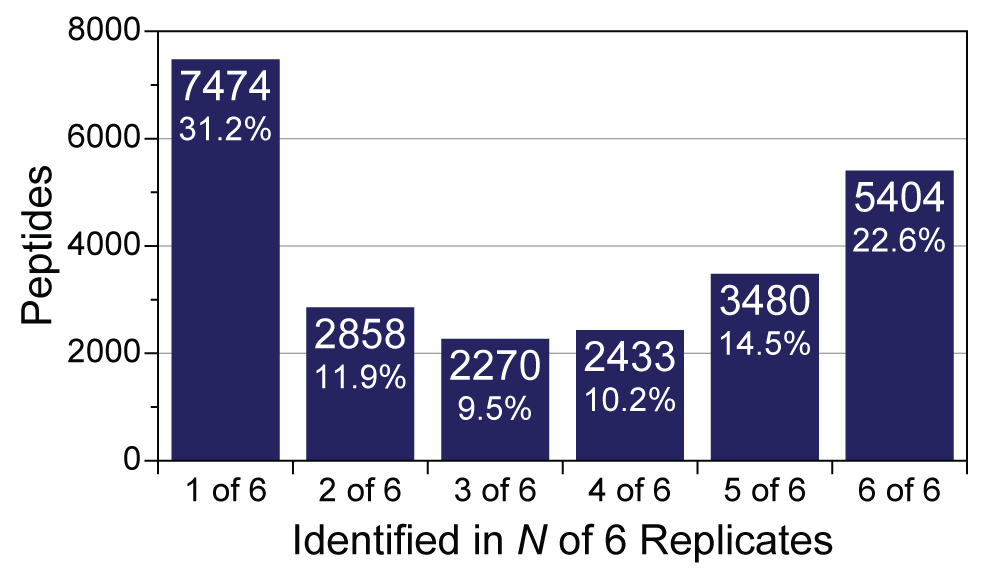
\includegraphics[width=\columnwidth]{eoa/EOA 1.png}
	\mycaption{Overlap of peptide identification among the analysis of six technical replicates}{Six nano-LC-MS/MS experiments produced 23,919 unique peptide identifications in total, but only one fifth of the identifications were observed in all six replicates. A large percentage (31.2\%) of the peptides were only detected in one of the six experiments.}
	\label{fig:eoa1}
\end{sidewaysfigure}
A significant portion were only identified once (7,474 31.2\%) while the remaining peptides were divided between two and five experiments. This clearly demonstrates the irreproducibility of DDA sampling on the same peptide solution. The reproducibility of identified protein groups fares better; 1,708 of 3,054 (56\%) protein groups were identified in every experiment. The higher overlap percentage is because many different peptides can make up one protein group, minimizing the importance of identifying the same peptides in all experiments. However, post translation modification (PTM) analysis requires identification of the same sites to compare between experiments, demanding the need for high peptide overlap. PTM analysis and quantitation is becoming more prominent in the literature, thus making this a growing problem in the field. Two reasons can be attributed to the poor reproducibility of stochastic DDA sampling. First, precursors having low signal-to-noise (S/N) are affected first by changes in chromatography and ionization. For example, a precursor with a maximal S/N of 4 may have been sampled and identified in one experiment, but in the next experiment the S/N may have dropped below the detection threshold and excluded from being sampled. This is evident when 8,883 MS1 features from peptides identified in one or all of the six experiments were examined for their maximal S/N (Figure \ref{fig:eoas1}).
 \begin{sidewaysfigure}[p]
 	\centering
 	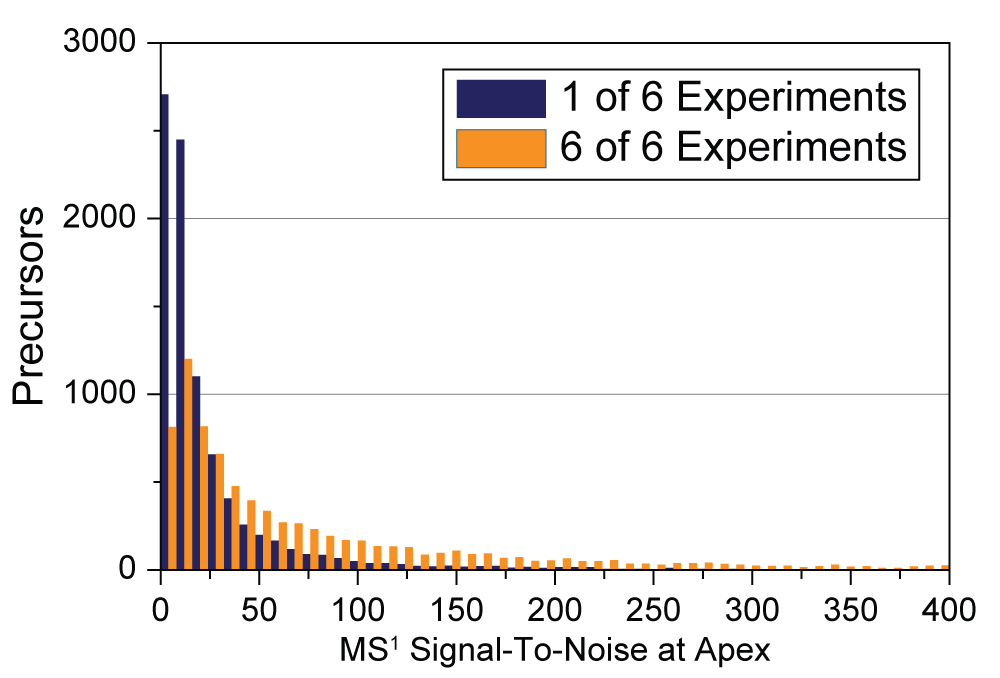
\includegraphics[width=0.9\columnwidth]{eoa/EOA S1.png}
 	\mycaption{Distribution of signal-to-noise ratios of reproducible and irrepoducible peptide identifications}{Peptides that were identified in 1 of 6 or 6 of 6 DDA top-15 experiments were analyzed for their maximal MS1 signal-to-noise (S/N). A larger percentage of those peptides seen only once appear at lower signal-to-noise values, indicating that MS1 signal intensity for reproducible identifications.}
 	\label{fig:eoas1}
 \end{sidewaysfigure}
For peptides identified once 2,707 (30.5\%) had a maximal S/N $\leq$ 4 while only 814 (9.2\%) precursors identified in every experiment had similar maximum S/N. The other reason for inconsistent peptide identification is increased MS1 spectral complexity, specifically its effect on charge-state assignment. In proteomic MS/MS workflows, precursors are often only selected when they exhibit a well-defined charge state -- usually where \textit{z} > 1, as singly charged precursors fragment poorly and usually do not lead to positive identifications. Increases in spectral complexity hinder the charge-state determination algorithms, especially for low S/N precursors. This results in skipping precursors even if its signal-to-noise is above the sampling threshold.

\subsection{Retention Time Based Targeting.}

When good peptide identification reproducibility is needed, retention time (RT) based targeting, i.e., scheduling, has been the method of choice. Here, peptides of interest are assigned an expected elution time and MS/MS are triggered, regardless of MS1 detection, during the appropriate time range. This avoids the two issues with DDA sampling described above and enables much higher reproducibility. However, such methods are laborious to construct and maintain identical LC and MS parameters must be kept between experiments to minimize any variances in retention times of the peptides.

To assess the degree of variance in peptide retention times that occur in normal nano-LC-MS/MS experiments, two of the yeast DDA experiments described above, performed nine days apart, were compared. The first experiment (July $22^{nd}$, D0) produced 13,529 unique peptides and the second experiment (July $31^{st}$, D9) identified 13,433 yeast peptides. Together, 7,589 peptides were in common and the apex of their retention time in each experiment is plotted in Figure \ref{fig:eoa2}A.
\begin{figure}[p]
	\centering
	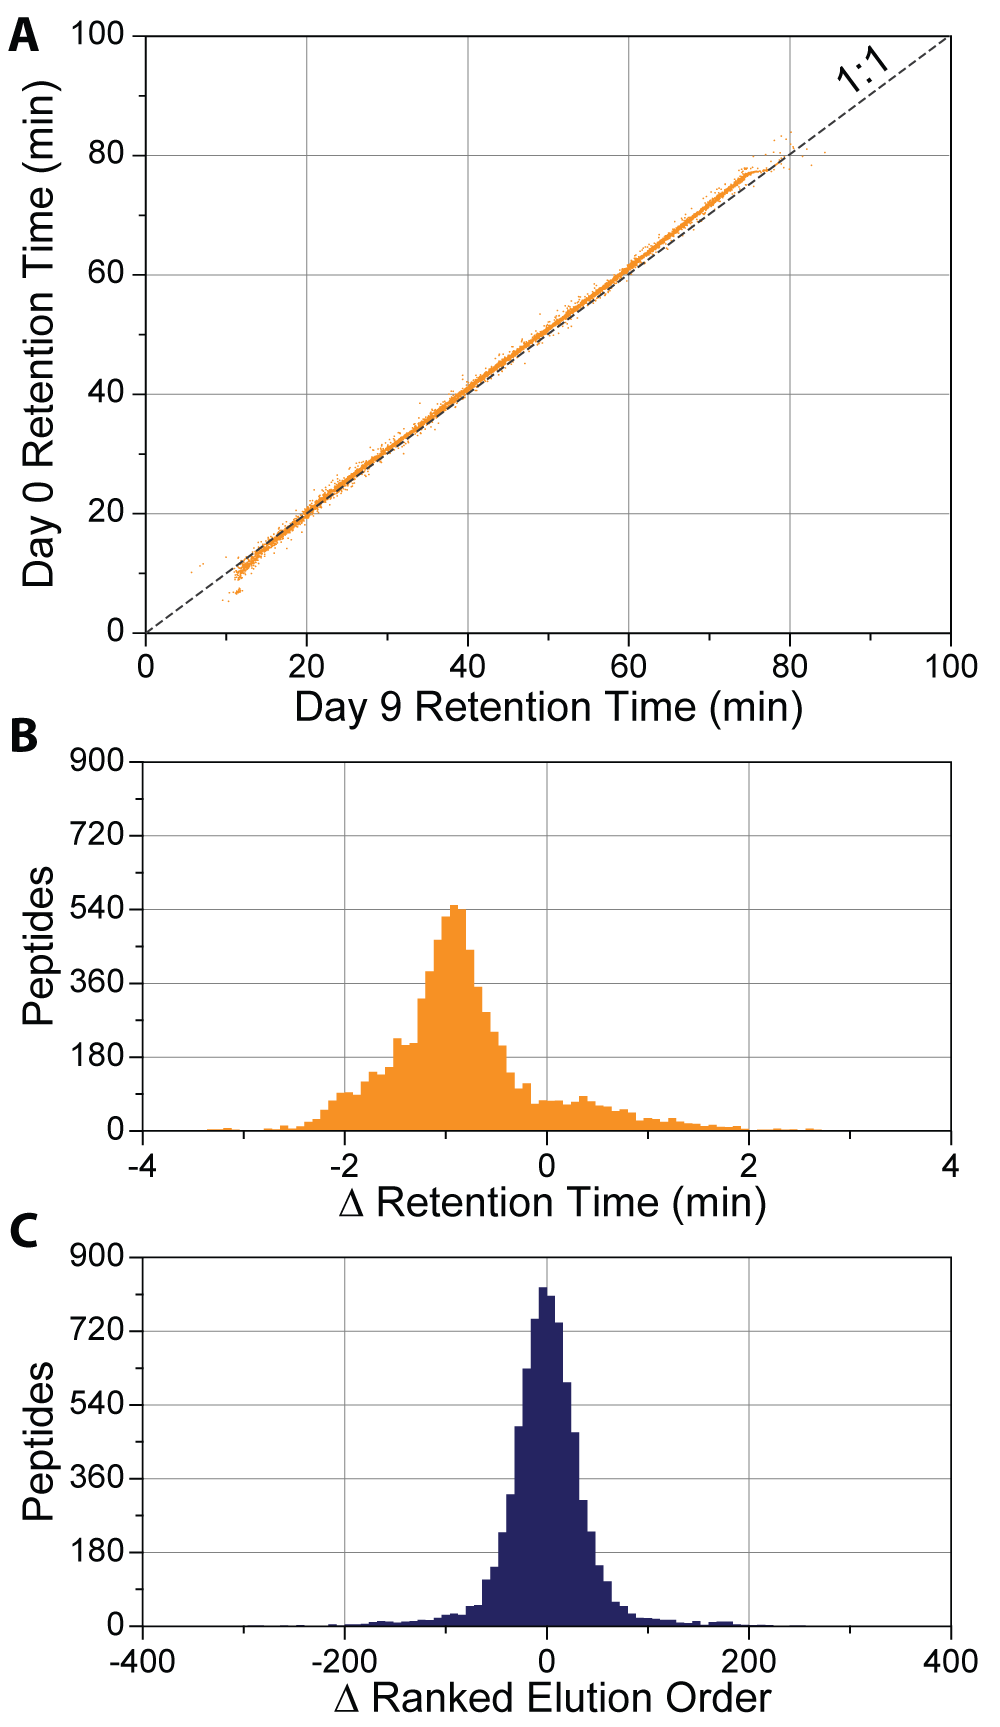
\includegraphics[width=0.65\columnwidth]{eoa/EOA 2.png}
	\mycaption{Retention time deviation between matched LC-MS/MS experiments}{To assess the deviation in retention times for matched samples two identical nano-LC-MS/MS experiments were run nine days apart on the same LC-MS system. (A) The relationship between apex retention times of the 7,589 unique peptides common between experiments display a high degree of linearity ($R^2$ = 0.9989) but a skewed slope and non-zero intercept (m = 1.033; b = -0.647).  (B) The average deviation from unity was nearly a minute off ($\mu$ = -0.805 min), with a broad distribution over 2 minutes wide. (C) Peptides ranked by their relative elution order exhibit a normal distribution around zero ($\mu$ =-1.097).}
	\label{fig:eoa2}
\end{figure} 

The relationship between retention times of matched peptides is highly linear ($R^2$ = 0.9989) but has a non-unity slope and non-zero intercept (m = 1.033; b = -0.647). While the slope is very close to 1, even the slightest deviation (0.033), compounded over time, leads to large RT differences late in the separation (e.g. \textasciitilde1.6 min shift at 70 min). On the whole, the average RT deviation was nearly a minute ($\mu$ = -0.805 min) with a broad distribution over a two minute range (Figure \ref{fig:eoa2}B). Typically, the assigned peptide elution times must be corrected to encompass this shift.

We hypothesize that -- due to the degree of linearity in peptide retention times,we could avoid these corrections by scheduling peptides based on their relative elution order (EO), opposed to their absolute retention time. Under similar LC conditions (i.e., same particles, temperature, column length, phase, etc.) peptides elute in the same relative order regardless of separation duration or slope. For example, if peptide 'A' elutes before peptide 'B' in a 30 minute LC gradient, the same ordering is preserved with a 60 minute LC gradient, even if the absolute retention times vary greatly. When many peptides’ elution orders are taken into account (e.g., 1000s of peptides) they provide a simple way to correct for elution variation dynamically. This is evident when we took the 7,589 peptides and rank ordered them based on their apex retention times for both the D0 and D9 experiments and plotted the difference between matched peptides (Figure \ref{fig:eoa2}C). Here the values are normally distributed around zero ($\mu$ =-1.097) with a full width at half maximum (FWHM) of only \textasciitilde100. Elution order can be useful even under extreme differences in chromatographic conditions as well.
\begin{figure}[p]
	\centering
	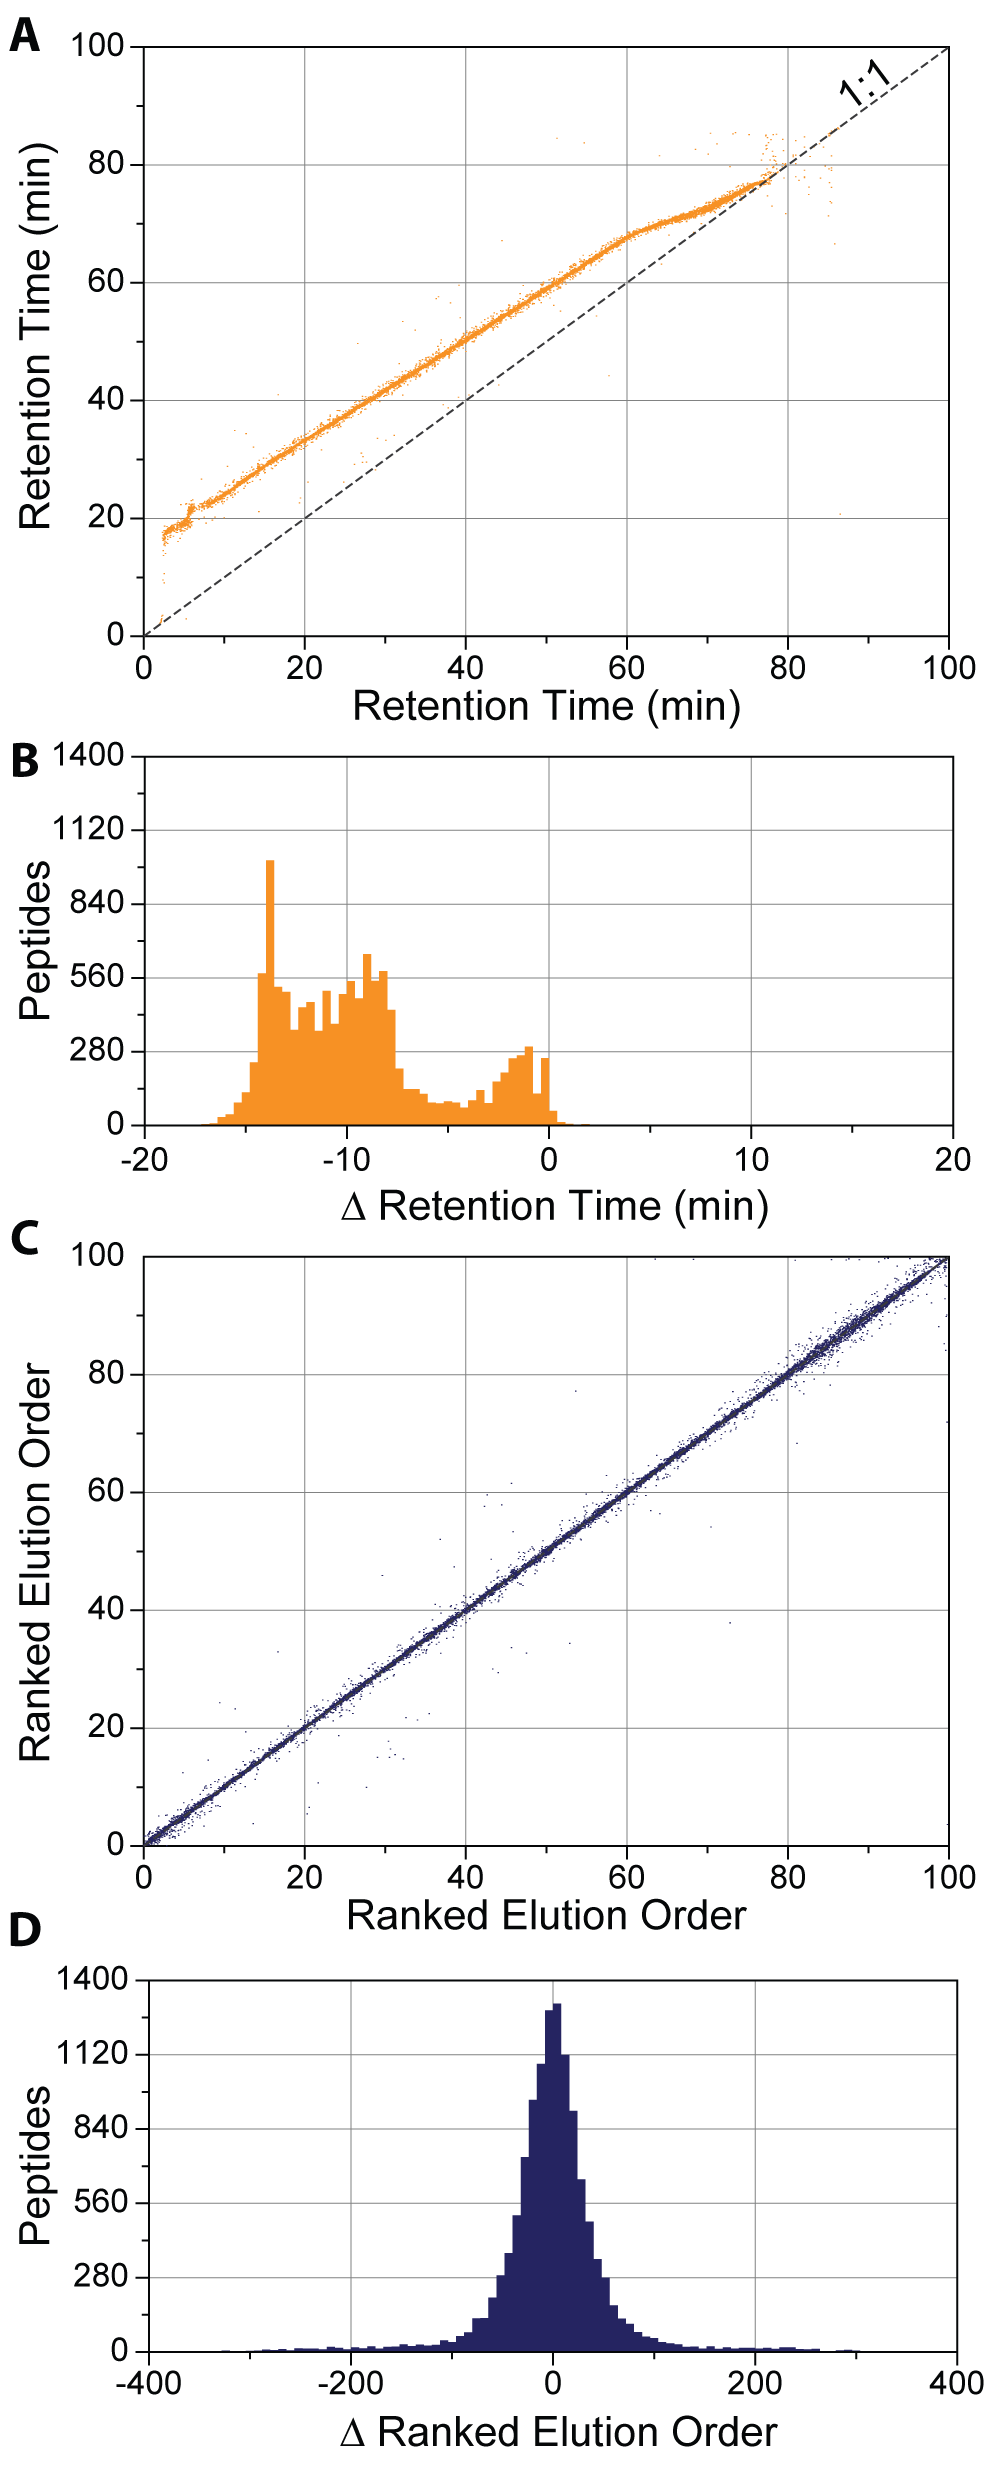
\includegraphics[width=0.5\columnwidth]{eoa/EOA S2.png}
	\mycaption{Two technical replicates of a yeast DDA top-15 method using two different LC gradients}{(A) Retention times for matched peptides between the two gradients is linear but not 1:1. (B) An average deviation of 10 min exists between the two experiments. (C) Rank elution orderings of matched peptides between the two gradients show a highly linear relationship that is exactly 1:1. (D) The average deviation in elution order for matched peptides is symmetric around 0.}
	\label{fig:eoas2}
\end{figure}

To simulate dynamic chromatographic conditions, we separated yeast peptides under two different LC gradient profiles. The resulting peptide identifications were again matched between the runs and the retention time difference was plotted (Figure \ref{fig:eoas2}A). These data show an average deviation of ten minutes between the two gradients (Figure \ref{fig:eoa2}B), but when ranked by their elution orders, the two experiments show a linear slope of 1 with a normal distribution of ranked elution orders around zero (Figure \ref{fig:eoa2}C\&D). 

\subsection*{Real-time Elution Ordering Alignment.}

We reasoned that using elution order could improve the irreproducible sampling of DDA -- similarly to scheduled methods, but on a larger scale and more robustly. The question shifts from ''what retention time is it?'' as scheduled methods ask, to ''what is the current elution order?'' By knowing which peptides are currently eluting from the LC, combined with the a priori knowledge of their elution order, we predict with high fidelity what peptides are going to subsequently elute. 

Prior knowledge is needed of the sample to adequately calculate the elution orders of the peptides in the sample. With time-based scheduled methods, many cursory experiments are performed to optimize the retention times of the targeted peptides. To reduce variances in retention times, it's vital that these initial experiments are conducted exactly the same as the targeted experiments. In stark contrast, elution orders can be determined using a variety of methods. First, much work has been devoted to determining peptide hydrophobicities from theoretical calculations of the amino acid sequence.\cite{ssrcalc,ssrcalc2,petritis,spicer} A simple list of peptides, ordered by their hydrophobicities, can produce a highly linear elution ordering. Second, previously collected data of the sample can produce an accurate elution ordering as long as the LC conditions are similar enough. This enables the combination of multiple datasets to produce a single elution order vs. \mz{} map (elution order map, EOM), regardless of their individual separation durations. This is accomplished by rank ordering all the peptide identifications in a given run and normalizing their orderings between 0 and 100 (where 100 represents the last eluting peptide). These normalized values are then matched between experiments and aligned using a simple algorithm to produce the final EOM as shown in Figure \ref{fig:eoa3}A.
\begin{sidewaysfigure}[p]
	\centering
	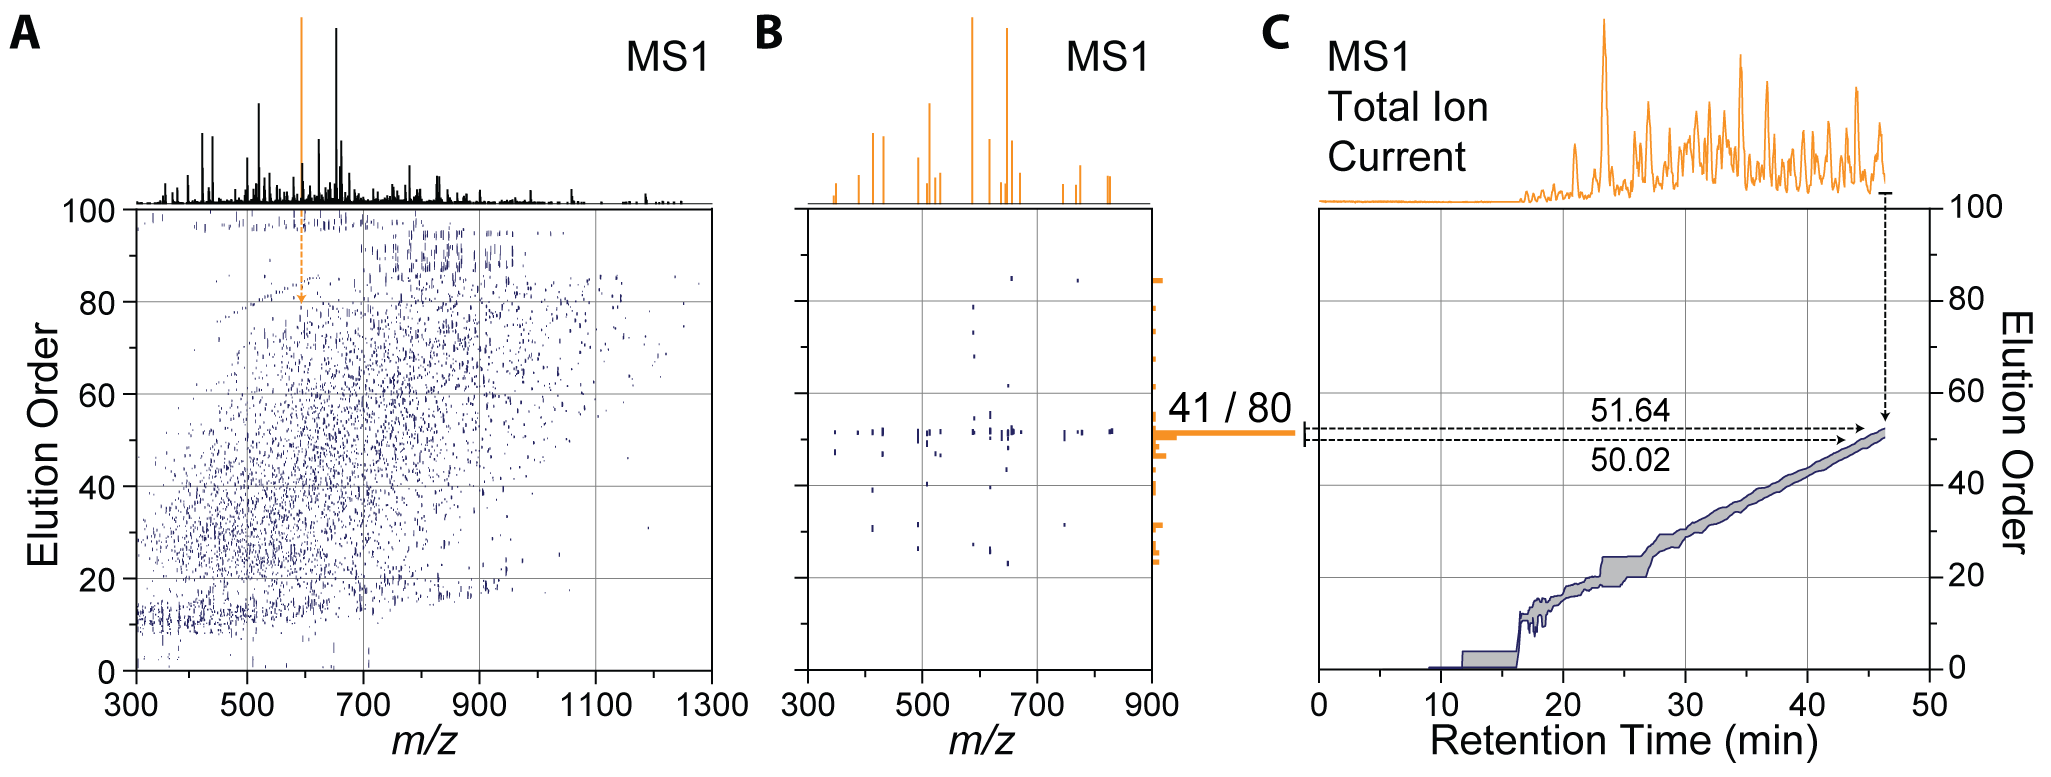
\includegraphics[width=\columnwidth]{eoa/EOA 3.png}
	\mycaption{Real-time elution order alignment algorithm}{After 46.3 minutes into a LC-MS/MS experiment, an MS1 scan is performed (A) and m/z features are matched to a 2D ion map stored on the instrument. (B) 21 of the peaks match 80 features in the ion map at a 10 ppm tolerance. Of these, over half (41 of 80) were mapped to one elution order bin (51 elution order). (C) A rolling elution order range is continually updated throughout the LC-MS/MS experiment.}
	\label{fig:eoa3}
\end{sidewaysfigure}
Lastly, the most robust method for determining peptide elution orders is to perform a discovery experiment right before the targeted experiment. Regardless of how elution order is determined, the final EOM is uploaded onto the instrument and is accessed throughout the course of the subsequent analyses.

Prior to targeted analysis, a list of peptide targets, along with their relative elution orders are also uploaded to the instrument (Figure \ref{fig:eoa4}B).
\begin{sidewaysfigure}[p]
	\centering
	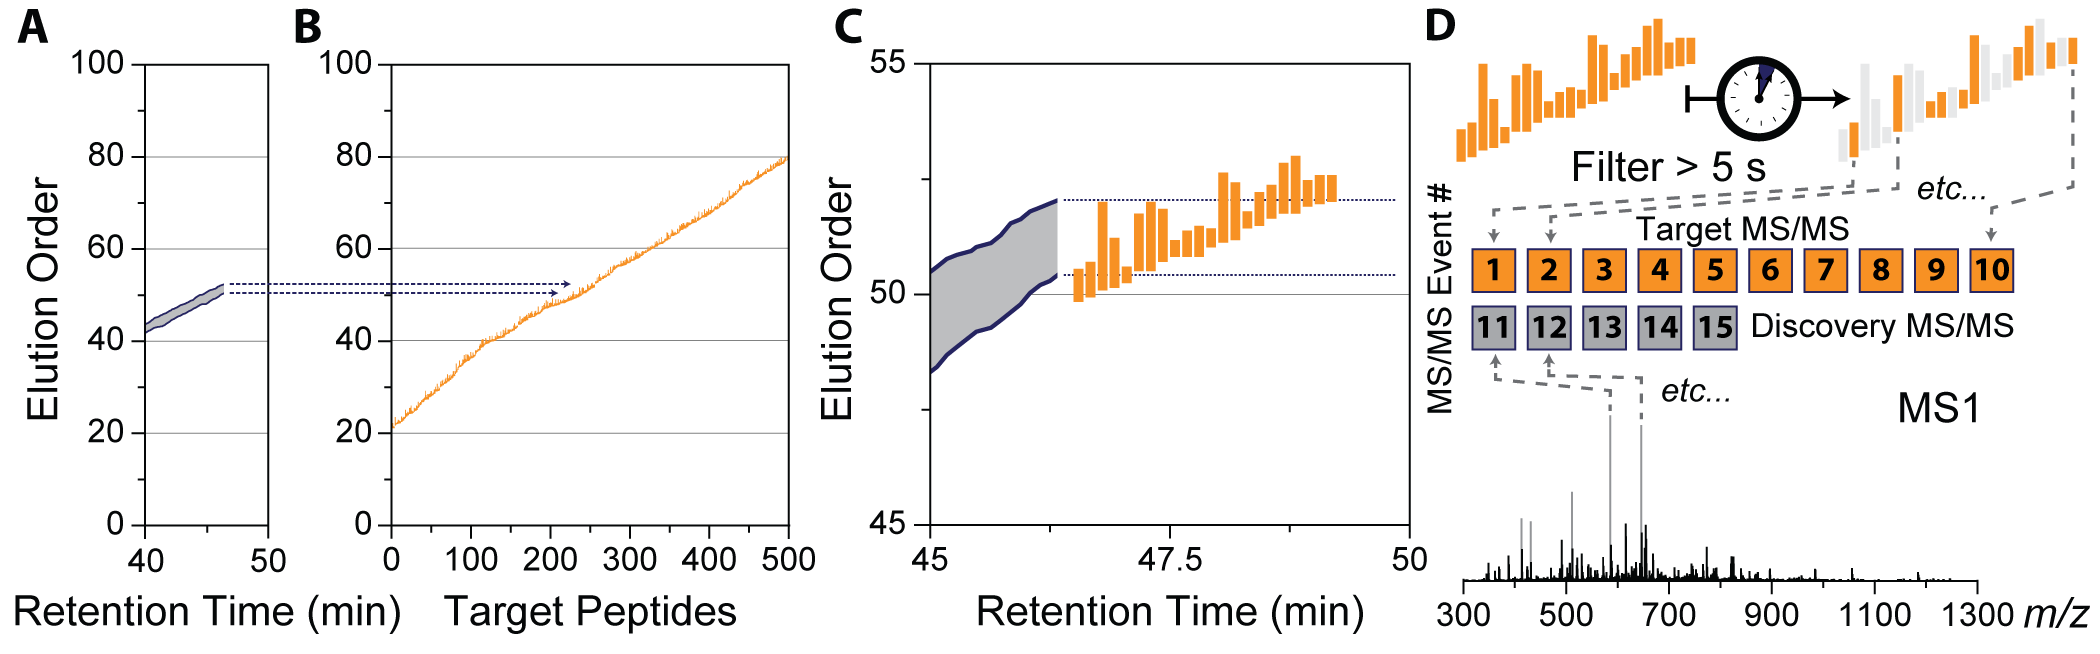
\includegraphics[width=\columnwidth]{eoa/EOA 4.png}
	\mycaption{Selection of targets within elution order range}{Following determination of the current elution order range (A), targets sharing a similar elution order are selected (C). Peptide targets within the elution order range are sorted based on when they were last sampled for MS/MS, leaving targets that have been waiting the longest. Those peptides are immediately sampled, regardless of MS1 detection (D). Remaining MS/MS events are automatically filled with DDA chosen m/z features.}
	\label{fig:eoa4}
\end{sidewaysfigure} 
Each target is assigned an elution order range depending on how long it was identified in the discovery experiments (see Figure \ref{fig:eoa4}C for zoom in). During the targeted analysis, instead of relying on absolute retention time to trigger targeted MS/MS, determining the current elution order becomes the main goal of the method. We have designed an online peptide elution order alignment (EOA) algorithm that takes a single MS1 spectrum and computes the current elution order therefrom. In brief, following MS1 acquisition, the EOA algorithm takes the most intense \mz{} feature and extracts all the elution order values from the uploaded EOM at a narrow \mz{} tolerance (e.g., 10 ppm) (Figure \ref{fig:eoa3}A). Each \mz{} feature is matched in a similar fashion and the resulting EO values are stored in a separate array (Figure 3B). In this example MS1, 21 \mz{} features matched a total of 80 EO values. When analyzed, 41 of these values are contained within a single 1 EO-wide bin. This indicates with high confidence that the current elution order is near this maximum. To determine the elution order precisely, the algorithm then calculates the 95\% confidence interval around the max EO bin and stores the minimum (50.02) and maximum (51.64) elution order. This process is repeated for each MS1 and over time the calculated elution order range constructs a rolling-average as shown in Figure 3C. The EOA algorithm is expedient, taking on average 26 ms per MS1 to execute and does not induce a statistically significant change in the total number of MS/MS scans performed (Figure \ref{fig:eoas3}).
\begin{figure}[p]
	\centering
	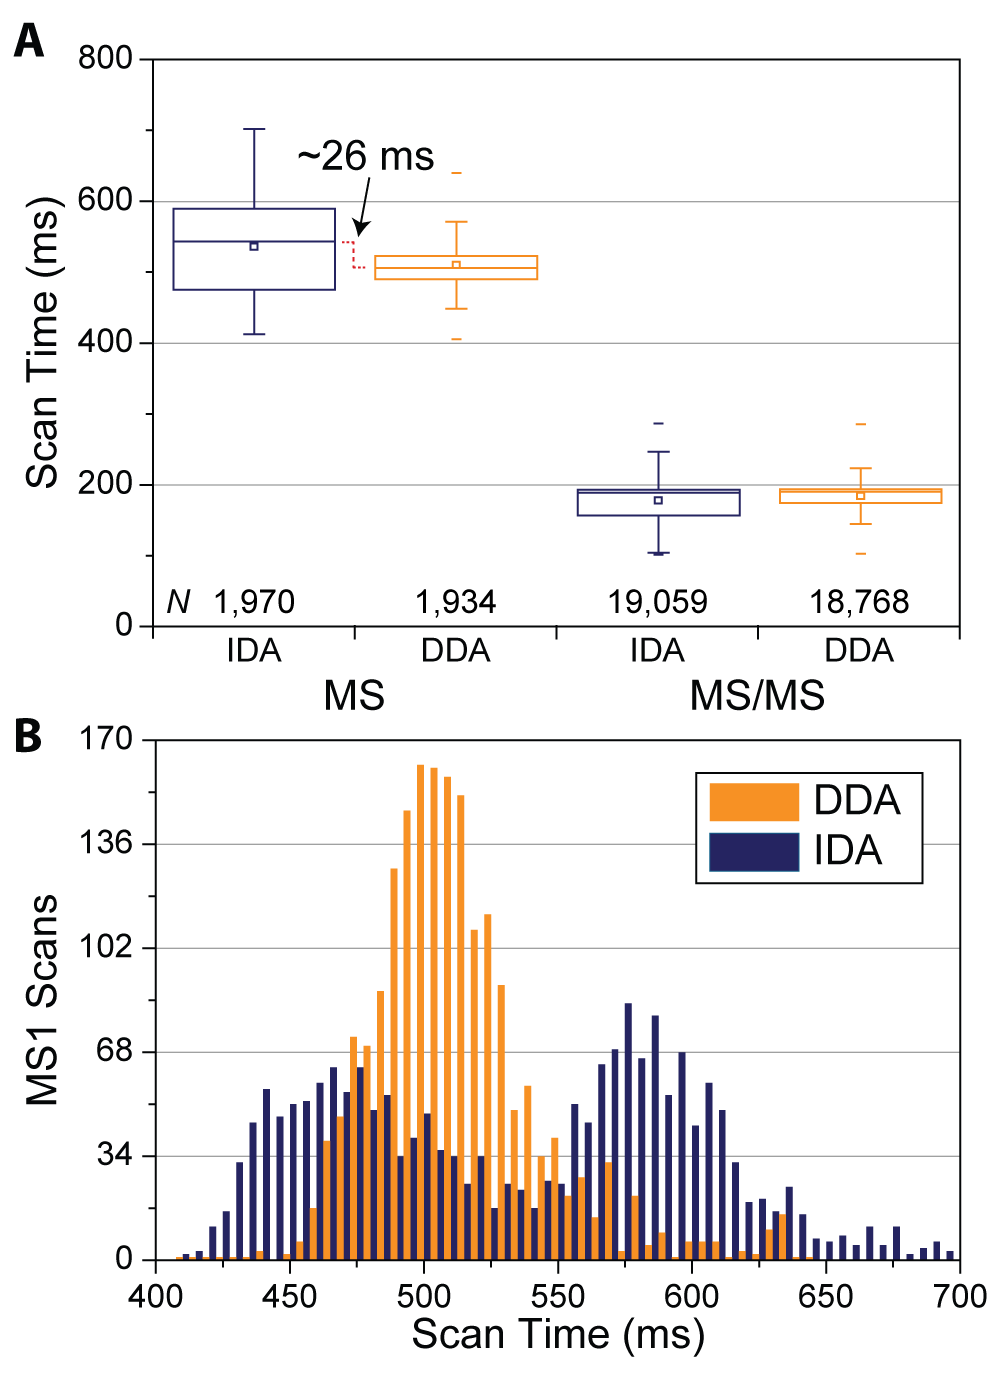
\includegraphics[width=0.8\columnwidth]{eoa/EOA S3.png}
	\mycaption{Duty cycle of elution order alignment algorithm}{(A) The elution order alignment (EOA) algorithm is expedient and induces only a slight increase in the MS1 duty cycle compared to normal DDA method (\textasciitilde26 ms). (B) The distributions of scan times for IDA is bimodal because the EOA algorithm can be triggered every other MS1, because the current elution order changes only slightly between consecutive MS1 scans.}
	\label{fig:eoas3}
\end{figure} 

Once the current elution order range is determined, peptides sharing a similar elution order are selected for MS/MS analysis. Briefly, the current elution order range is intersected with the target peptides already uploaded on the instrument (Figure \ref{fig:eoa4}B) and overlapping peptides are stored as potential targets (Figure \ref{fig:eoa4}C). These peptides have a high probability of eluting next since they share very similar EO values with the current overall EO value. Since there can be many potential targets at any given time, they are filtered based on how long since they were last sampled, this is to prevent oversampling of any one target. Peptides that have been waiting the longest (i.e., > 5s) are automatically triggered for MS/MS analysis regardless of MS1 detection. Unfilled MS/MS events are then populated using normal DDA top-N approaches, excluding any \mz{} previously selected to be targeted (Figure \ref{fig:eoa4}D). This data collection scheme enables repetitive, consistent targeting of multiple peptides over their elution, while allowing DDA scans to facilitate discovery. Quantitative strategies such as PRM can be used in conjunction with the EOA algorithm (Figure \ref{fig:eoas4}).
\begin{figure}[p]
	\centering
	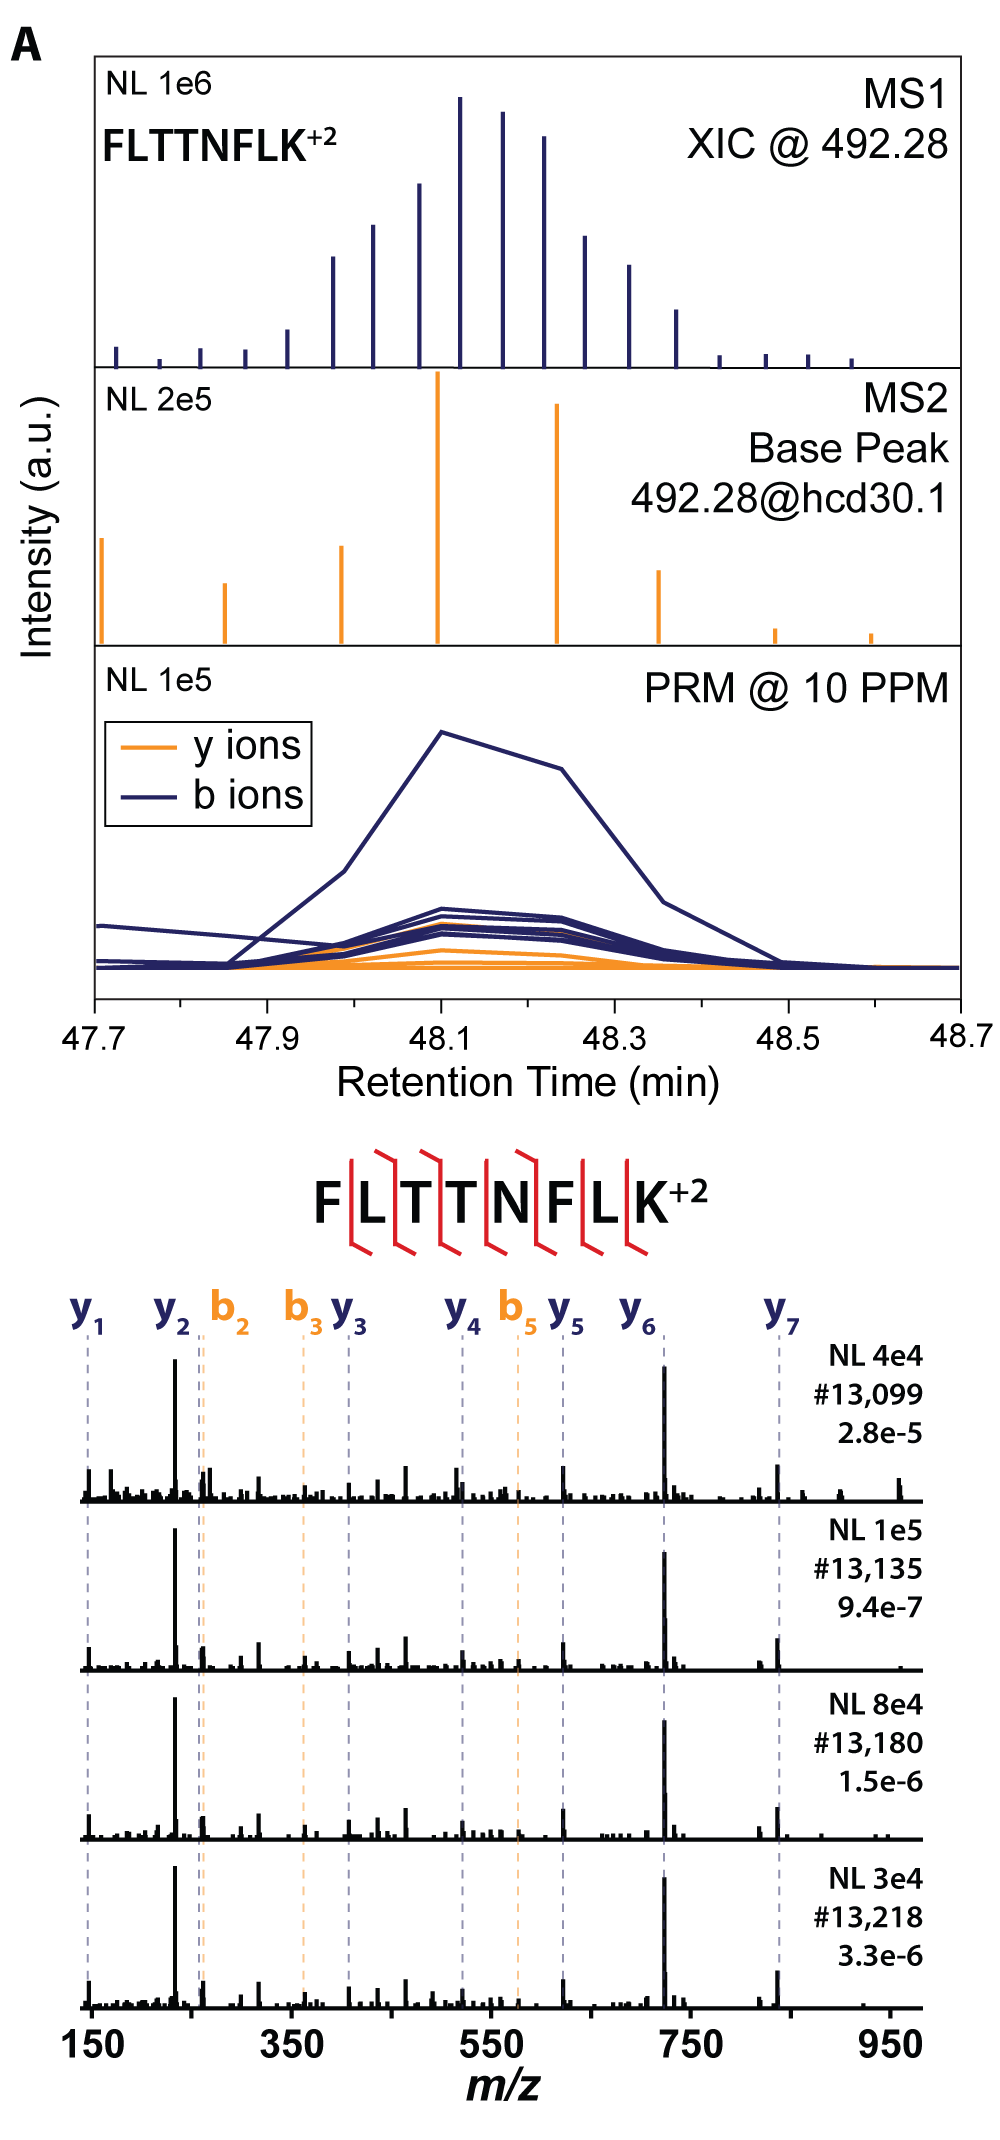
\includegraphics[width=0.6\columnwidth]{eoa/EOA S4.png}
	\mycaption{Parallel reaction monitoring (PRM) scan sequences obtainable using the IDA method}{(A) The peptide FLTTNFLK was MS/MS sampled approximately every 6 seconds over its elution profile. The b- and y-ions intensities were tracked over time to provide quantitative results.}
	\label{fig:eoas4}
\end{figure}  

\bibliographystyle{ieeetr}
\bibliography{eoa}
\chapter{Software Frameworks for Proteomic Data Analysis}



\section{Summary}
Proteomic research can be divided into three major divisions: 1) sample generation and preparation, 2) mass spectral data collection, 3) and data interpretation and analysis, each with its own set of challenges. While improvements in both sample preparation and instrumentation have greatly propelled the field forward, data analysis software has developed at a slower rate. This may be a result of competing standards of data storage and access, the shear complexity of large-scale data, or the simple fact that a majority of scientists are not programmers. Whatever the case may be, automatic data analysis is a needed part of the equation, an integral step to help answer large and meaningful biological problems. The existence of software is not final goal, the tools must be simple-to-use yet powerful, flexible yet robust, accessible yet timely in order to gain traction and be impactful to the field. To meet these demands, the following chapter describes the development of two open-source software packages used in proteomic data analysis. The first package is the Coon OMSSA Proteomic Analysis Software Suite (\compass{}), a graphical program used to analyze proteomic data from initial spectral processing all the way to protein quantitation. It is geared for the end user to process their data in a straightforward, but flexible manner. The second package is devoted to developing new software tools in a timely fashion and is called C\# Mass Spectrometry Library (\csmsl{}). This programming toolbox offers a wide range of proteomic and mass spectrometry tools and methods for developing new software analysis tools. It is powerful to handle the most complex data, but approachable enough that even novice programmers can use it with minimal training. These two software tools are still in their infancy, but are constantly being updated and maintained to meet the needs of the ever-changing proteomic landscape.

\section{Introduction}
In many scientific disciplines, as the complexity of the problems grow, so to does the informatic resources to keep pace. Proteomics and mass spectrometry are no exception. As researchers aim to answer larger biological problems on grander scales, proteomic data analysis needs to keep up. The mass spectrometers used to collect the data are becoming faster and more sensitive (i.e., more data) with each passing year. Acquiring 20 MS/MS spectra per second is now possible. These mass spectrometers are also becoming more robust and powerful, enabling them to be continually ran for days and days at a time with very little down time. In the end, hundred of thousands of spectra are collect per instrument in an average day, totaling millions over a week. Keeping up with this volume of data requires sophisticated software and data management tools. These tools must be powerful enough to handle the complexity of the data, flexible to changes and updates in how data is analyzed, and simple enough that non-programmers can efficiently use them. 

To meet these requirements, the Coon research group has developed a range of software tools to analyze mass spectrometry data. First, our group has previously published a suite of software tools called Coon OMSSA (Open Mass Spectrometry Search Algorithm) Proteomic Analysis Software Suite (\compass{}).\cite{compass} The suite encompasses all the basic tools for analyzing mass spectrometry-based proteomic data. It handles the spectral cleaning and conversion, supports MS/MS searching (\emph{via} OMSSA\cite{omssa}), false discovery analysis, protein grouping, various types of quantitation, post-translational modification localization, and protein quantitation, among others. To handle the massive number of spectra collected by a host of users per day, we have utilized the High Throughput Condor (HTCondor) system--developed here at the University of Wisconsin-Madison, to greatly speed up our database searching program by simultaneously using hundreds of computers across campus. Since its initial publication, \compass{} has been heavily upgraded and expanded to meet the changing needs of the group. This chapter summarizes the different programs of \compass{} and the changes and updates made to them since the publication version of the software.

The second software tool we have developed is an open source programming library specifically designed for proteomic data analysis called C\# Mass Spectrometry Library (\csmsl{}). This library speeds up the development of software, providing many common functions and concepts needed for data analysis (e.g., peptides, chemical formulas, spectral searching, etc.). This removes the burden from the programmer to reinvent the wheel each time data needs to be analyze. Each of its features have been carefully designed and tested to provide a powerful, flexible, and robust set of tools for programmers to use. We kept the design of the library to be as simple as possible, enabling even novice programmers to quickly analyze their data in unique fashions with little training. Given the complexity of proteomics and mass spectrometry, this allows the user to focus more on the scientific data than the management and construction of complex software. In this chapter, the concept and design of \csmsl{} will be outlined and a few coding examples are provided to show the simplicity of the library. \csmsl{} is a work ongoing, and the version at the time of this publication (v0.2.1) is far from its final form. 

\section{COMPASS: Coon OMSSA Proteomic Analysis Software Suite}
The \compass{} program is a complete, standalone data analysis platform for proteomic mass spectrometry. It is based around the Open Mass Spectrometry Search Algorithm (OMSSA) as the primary MS/MS search engine, but has been partially adapted to handle inputs from other proteomic search engines (e.g., SEQUEST, Proteome Discoverer).\cite{sequest} It is written for the Windows operating system using their .NET Framework (v3.5 and above) in the C\# programming language. The complete source code is available at \url{https://github.com/dbaileychess/Compass} and the current version is v1.2.12 at the time of this publication.
\begin{figure}[p]
	\centering
	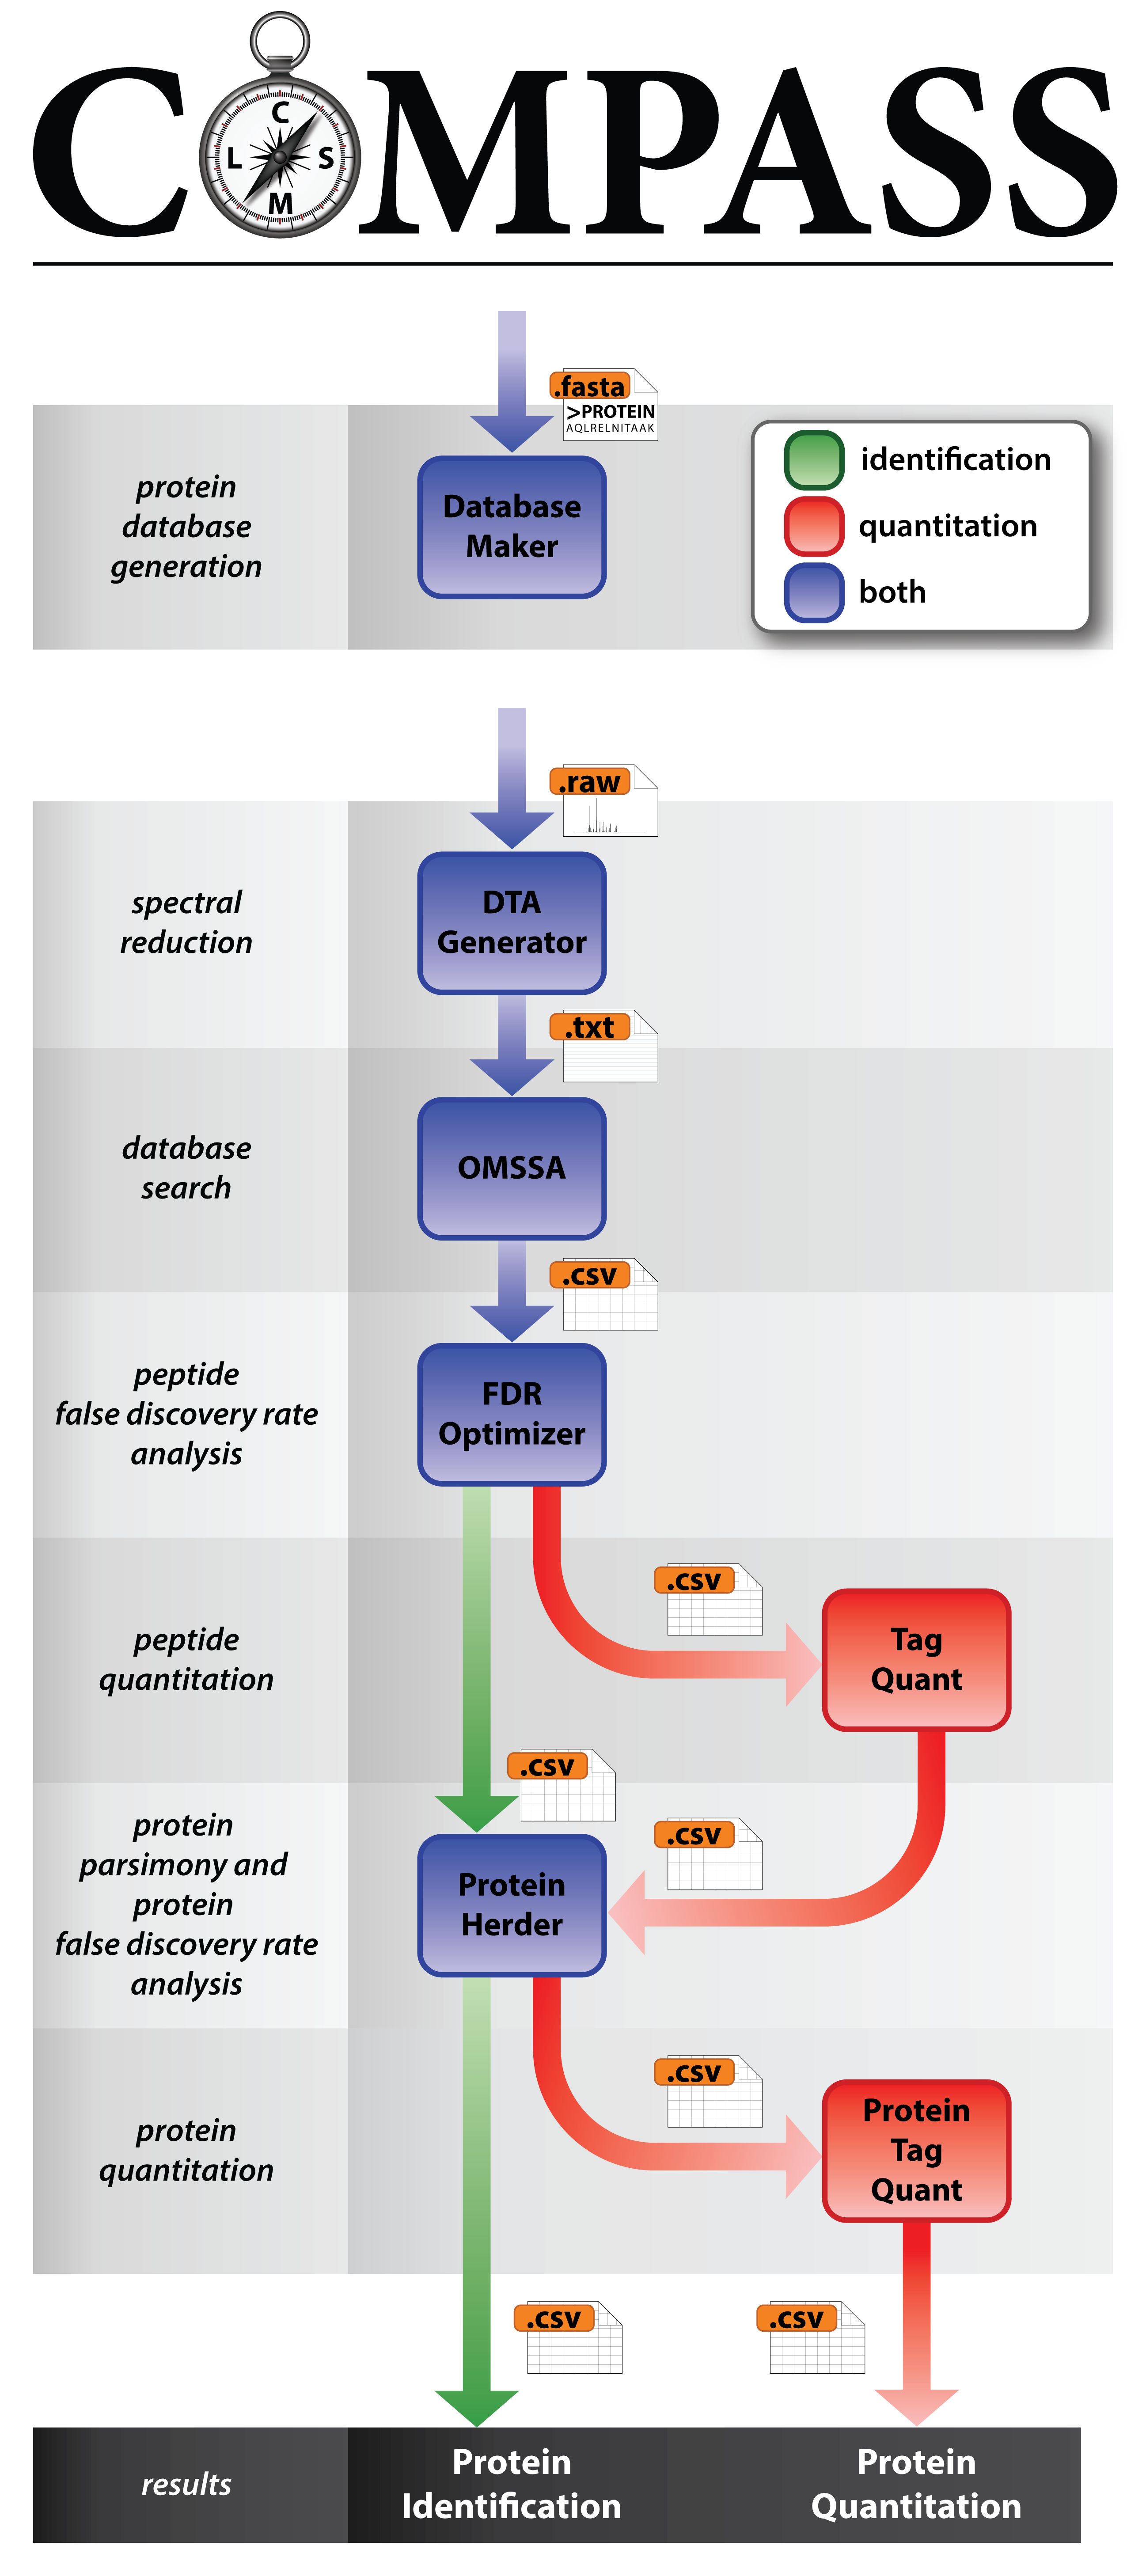
\includegraphics[width=0.5\columnwidth]{csmsl/compass.png}
	\mycaption{Analysis workflow of \compass{}}{\texttt{Database Maker} generates BLAST-formatted protein databases for OMSSA. \texttt{DTA Generator} converts raw instrument data to text files for searching with OMSSA. \texttt{FDR Optimizer} performs FDR analysis at the spectrum/peptide level, followed by protein parsimony and FDR analysis at the protein level with \texttt{Protein Herder}. For quantitation, the workflow is supplemented by \texttt{TagQuant}, which performs spectrum/peptide-level quantitation, and \texttt{Protein TagQuant}, which performs protein-level quantitation.}
	\label{fig:compass}
\end{figure}
The application contains an graphical user interface (GUI), making it very intuitive and easy to use. \compass{}  contains several other GUI programs, each corresponding to a separate step in the analysis. Users process data files through each individual program, which typically writes the result of the analysis to different files and folders on the computer. Other programs then process those result files to add additional analysis and outputs. This design enables customized analysis worflows to handle the various types of analysis commonly used (Figure \ref{fig:compass}). 



\compass{} was first published in 2011, but has been substantially upgraded to improve the user experience, fix bugs, introduce new features, and for general execution improvements. The program was also heavily refactored (code reorganization) to ease future maintenance. The following sections summarize the different parts of \compass{} and the improvements made to them from the initial publication.
 

\subsection*{Database Maker.}
\texttt{Database Maker} creates protein databases for target-decoy searching of MS/MS spectra. Text files containing each protein sequence, in the \texttt{.fasta} format, are converted to a decoy version of the same length by reversing, shuffling, or generating random amino acids.\cite{targetdecoy,targetdecoycomp,qscore} The decoy sequences are then concatenated to the input file and exported to another \texttt{.fasta} file. Additionally, protein sequences can be converted to the basic local alignment search tool (BLAST) format for use with OMSSA.\cite{blast} The GUI portion of the program (Figure \ref{fig:databasemaker}) has been restructured to enable multiple \texttt{.fasta} files at the same time. Internally, \texttt{Database Maker} now uses the \texttt{makeblastdb} program to generate BLAST databases instead of the now deprecated \texttt{formatdb}, both of which are provided by the National Center for Biotechnology Information (NCBI).
\begin{figure}[p]
	\centering
	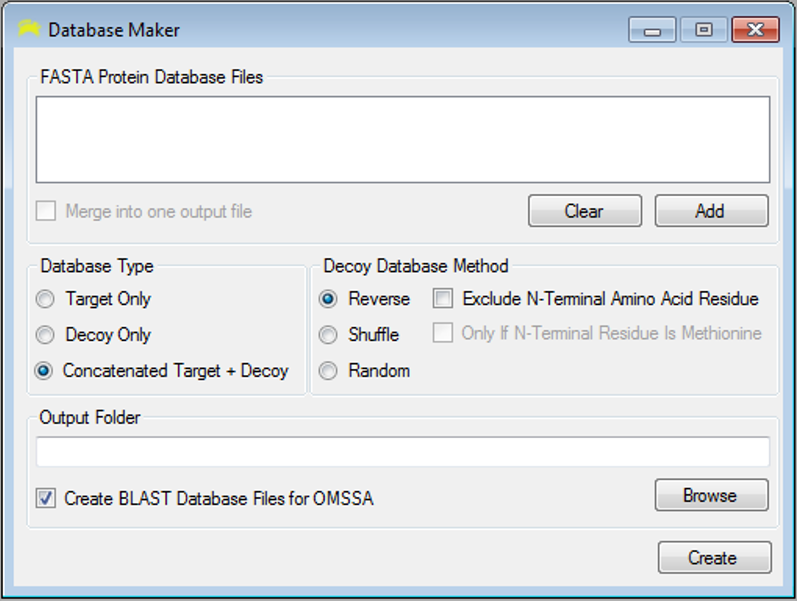
\includegraphics[width=\columnwidth]{csmsl/databasemaker.png}
	\mycaption{Database Maker}{The GUI program used to manage, construct, and modify protein databases in the \texttt{.fasta} format. It is capable of constructing various forms of decoy databases used for false discovery analysis. An optional BLAST database can be produced for compatibility with OMSSA searching.}
	\label{fig:databasemaker}
\end{figure}

\subsection*{DTA Generator.}
The second program in the \compass{} workflow is \texttt{DTA Generator}, which reduces LC-MS/MS spectral data to \texttt{.txt} files for database searching (Figure \ref{fig:dtagenerator}). Various peak cleaning algorithms are used to simplify spectral prior to searching, these include removal of unreacted precursor, electron-transfer dissociation (ETD) pre-processing to remove precursor, charge-reduced precursors, and neutral losses from charge-reduced precursors.\cite{good} The outputs generated by the software are also usable by several search algorithms. Although OMSSA is our focus, individual \texttt{.dta} files for SEQUEST or \texttt{.mgf} files for MASCOT are possible outputs.\cite{sequest,mascot}

Since the initial publication, additional spectral filters have been added to allow the user more freedom in how the spectra are processed. These include specifying neutral loss products and isobaric label clean up. The most significant improvement to DTA Generator since publication was a dramatic decreased in execution time (\textasciitilde50X). This was accomplished by converting the code to utilize multiple processor threads, as well as algorithmic improvements to spectral cleaning. 
\begin{figure}[p]
	\centering
	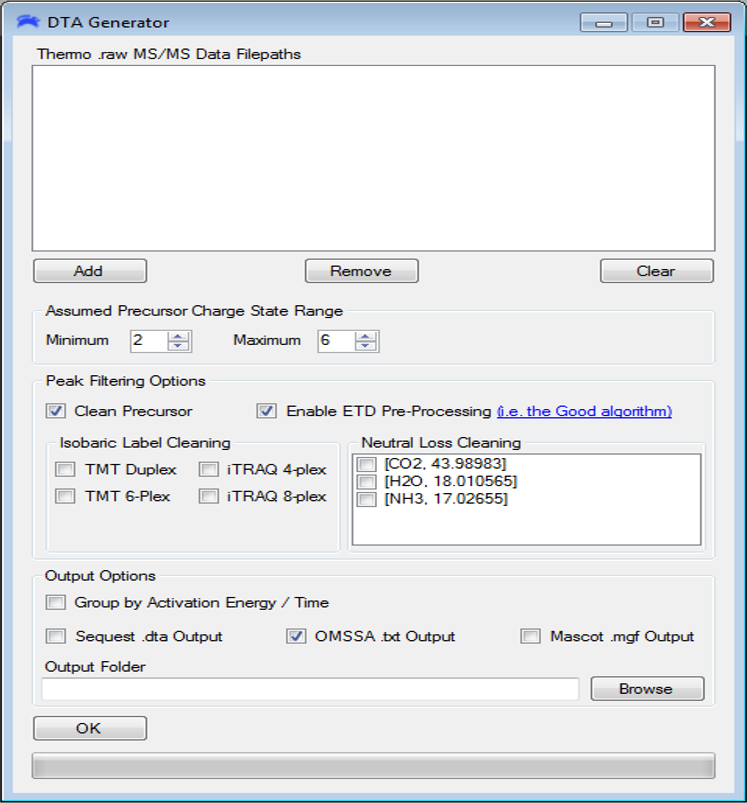
\includegraphics[width=0.8\columnwidth]{csmsl/dtagenerator.png}
	\mycaption{DTA Generator}{The program takes spectral data in Thermo's \texttt{.raw} format and generates a \texttt{.txt} of the processed spectra. Processing includes removing peaks that do not provide sequence-informative results (i.e., neutral loss). The program is capable of producing outputs for OMSSA, SEQUEST and Mascot search algorithms.}
	\label{fig:dtagenerator}
\end{figure}

\subsection*{Open Mass Spectrometry Search Algorithm.}
\texttt{OMSSA} is a database search algorithm for proteomic datasets developed at the NCBI by Lewis Geer.\cite{omssa} It uses a probabilistic scoring to assign confidence that a specific peptide sequence best fits to the experimental spectrum. The program assigns an expectation value (e-value) to each peptide spectrum match (PSM) generated, stating the probability of matching that sequence to the spectra by random chance. The smaller the e-value, the higher the confidence that a peptide with a certain sequence produced the MS/MS spectra. Further statistical analysis is performed in the \texttt{FDR Optimizer} program, discussed below. OMSSA provides the option to produce a \texttt{.csv} output of all the PSMs generated (\texttt{-oc}). This format is the basis for all the other programs in \compass{}. It is easily opened and manipulated by spreadsheet programs (e.g., Microsoft Excel) and is human readable. This is in contrast to a majority of other proteomic software, where \texttt{.xml} or a proprietary format is preferred.

\subsection*{High Throughput Condor for OMSSA.}
Arguably the biggest improvement to \compass{} since publication is the addition of the High Throughput Condor (HTCondor) system for improving OMSSA searching times. In brief, HTCondor is a computational management system for scheduling processing jobs across a distributed network of computers. Here computers voluntary join a HTCondor network which enables them to donate their free CPU cycles to other processes, increasing the overall processing power of the network. The processing power of the network scales with the size of the network. This is ideal for large universities, where there is a large number of computers on a common network, and a majority of those computers (e.g., computer labs, servers, kiosks, office computers) are not in use 24-7. The HTCondor system intelligently monitors CPU activity on each attached computer, and given a certain amount of inactivity, reassigns its CPU to process jobs waiting in a global job queue. If HTCondor detects new local activity on that computer (e.g., keyboard or mouse movement, a local processing job, etc.), it will either pause the global job, or automatically transfers it to another inactive computer. Given the large size of the HTCondor network on the University of Wisconsin-Madison campus (~7,000 CPUs) there is a high probability that there will always be multiple computers available for analysis. This large network provides million of CPU hours to researches all across campus. From the HTCondor website, they state that ''from July 2011 to June 2012, the [Center for High Throughput Computing] provided 70 Million CPU hours to campus researchers and off-campus collaborators.''

Shortly after \compass{} was published, we developed a GUI program called \texttt{Coondornator} to provide a method for searching MS/MS data \emph{via} OMSSA over the University of Wisconsin-Madison's HTCondor network. The program first transfers \texttt{.dta} files (generated by \texttt{DTA Generator}) from a user's computer to the Coon Group fileserver, which is its own 17-CPU HTCondor network. If these computers are idle, they automatically start processing each submitted OMSSA job. If more than 17 OMSSA searches are submitted at once, overflow jobs are automatically routed to the Center of High Throughput Computer (CHTC) HTCondor cluster (\textasciitilde6,800 CPUS) for analysis. When the OMSSA searches are completed, the resulting \texttt{.csv} file containing all the PSMs are transferred back to the Coon Group fileserver for storage. This program provides a seamless integration between the HTCondor network and end user's computer, making high throughput computing no harder than running a program on their computer. The Coon Group routinely searches hundreds of \texttt{.dta} files containing million of spectra on the HTCondor network each week.

Typically, users would search all the MS/MS spectra from a single LC-MS/MS experiment on their desktop computers. With HTCondor, a single LC-MS/MS experiment is broken up into smaller sets of spectra (e.g., 1000 spectra per set) and search individually and then recombined when all the searches are complete. This represents a significant throughput gain compared to searching files on individual desktop computers. Conservative estimates is about 30-50X boost in execution times on average. For example, to search all the MS/MS spectra from a one hour LC-MS/MS experiment of a tryptic digestion of whole-cell yeast cells would take about 30-40 minutes on a normal desktop computer. In contrast, if all the MS/MS spectra were split into groups of 1000 spectra each, and searched using \texttt{Coondornator} over the distributed HTCondor network, the same results could be generated in \textasciitilde1 minute, a 30X decrease in execution time.

\subsection*{FDR Optimizer.}
\texttt{FDR Optimizer} filters PSMs generated from \texttt{OMSSA} to control for false identifications (Figure \ref{fig:fdr}). The program maximizes the number of true positive identifications at a given error rate, typically set to under 1\%. \texttt{FDR Optimizer} can work on either low-resolution MS1 data with a simple e-value filter, or on high-resolution MS1 data with a two dimensional filter on precursor mass error and e-value. To use \texttt{FDR Optimizer}, both target and decoy protein sequences have to be searched with \texttt{OMSSA} on the same set of spectra for adequate false discovery filtering. 
\begin{figure}[p]
	\centering
	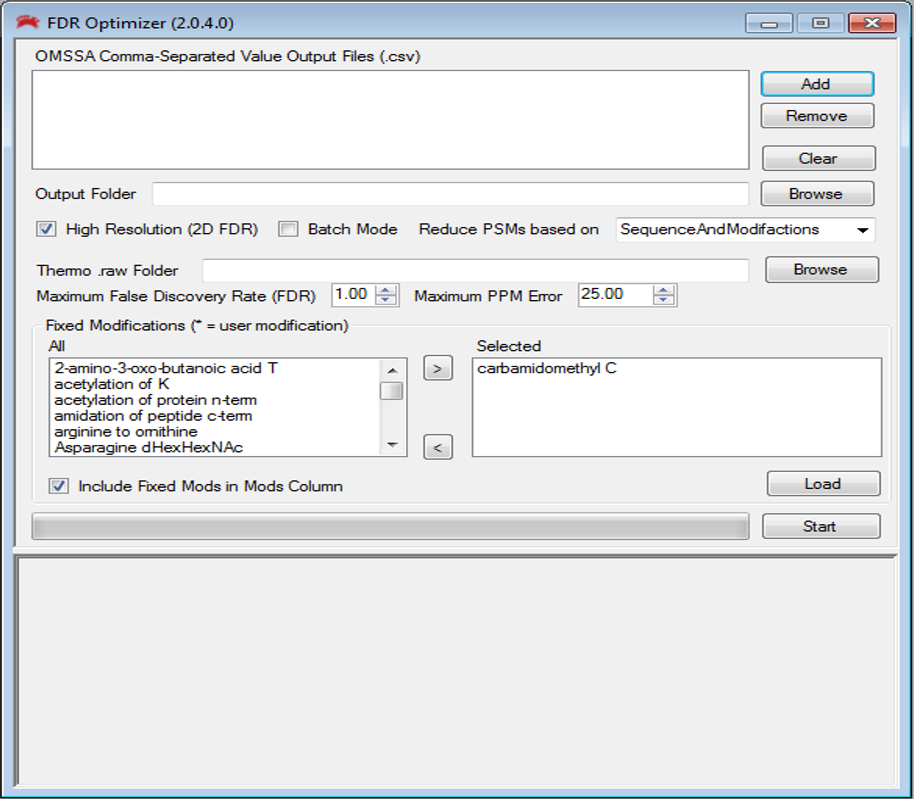
\includegraphics[width=\columnwidth]{csmsl/fdr.png}
	\mycaption{FDR Optimizer}{The new GUI for \texttt{FDR Optimizer}, this version combines all four versions into one program for a simplified user experience.}
	\label{fig:fdr}
\end{figure}

For low-resolution datasets, PSMs are first loaded into the program and the best scoring PSM (i.e., lowest e-value) for each spectrum is saved and all other PSMs are discarded. The remaining PSMs are then sorted on their e-value, from smallest to largest. Each PSM also has a flag to indicate whether it resulted from a target protein or a decoy protein. A counter for both the number of targets ($T$) and decoy ($D$) peptides identified is kept as the program iterates over the sorted PSMs. When the false discovery rate (FDR, Equation \ref{eq:fdr}) increases over some specified value (e.g., 1\%), the program stops the iteration.
\begin{equation}
FDR =\frac{D}{T + D}
\label{eq:fdr}
\end{equation}
The PSMs that have been already been processed are then outputted to a \texttt{.csv} file and represents the true identifications. Known decoy peptides that pass this filter are exported to a decoy-specific \texttt{.csv} file that is used later for protein-level FDR analysis.

High-resolution MS1 datasets can be processed with an additional filter to increase the number of identifications. First each PSM is read into the program and its precursor mass error is determined from the MS1 spectrum. The median precursor mass error of all PSMs is then computed and each PSM is corrected by this median value. This corrects any systematic mass error the mass spectrometer had, and usually reduces the mass errors to under 5 ppm. \texttt{FDR Optimizer} then iteratively sets a maximal ppm error allowed (i.e., from 1 to 100 ppm), and filters the PSMs to contain only precursor mass errors lower than the maximum. These filtered PSMs are then processed identically to the low-resolution dataset described above. This whole process is then repeated with a slightly larger maximal ppm error, and the number of identifications is recorded. The program tries all possible maximal ppm errors and reports the ppm error that produced the most true identifications at the end. This maximizing algorithm increases the number of true identifications produced then the simple low-resolution filter.

Since publication, \texttt{FDR Optimizer} has been completely rewritten. Previously, four separate programs were used and maintained: \texttt{Low-Resolution FDR Optimizer}, \texttt{FDR Optimizer}, \texttt{Batch Low-Resolution FDR Optimizer}, and \texttt{Batch FDR Optimizer}. The current version simplifies the user experience by combining all four programs into one, with simple option check-boxes to indicate the desired analysis (Figure \ref{fig:fdr}). Improvements to the FDR analysis and maximizing algorithms have also lead to a large decreases in execution times (\textasciitilde10-20X).

\subsection*{TagQuant.}
The \texttt{TaqQuant} program extracts and processes isobaric labeling quantitative information from MS/MS spectra (Figure \ref{fig:tagquant}). It is compatible with both major types of isobaric labels, TMT and iTRAQ.\cite{tmt,itraq} \texttt{TagQuant} obtains intensities of the reporter ions of interest from the raw data. These intensity values are subsequently denormalized by multiplying by the ion injection time to yield the number of ion counts detected, a quantity which can be fairly compared across different spectra and analyses. Purity correction is then applied using user-specified purity data provided by the manufacturer.\cite{itracker} Finally, normalization is performed such that the total intensity of each tag is equal, accounting for differences in sample mixing quantities.
\begin{figure}[p]
	\centering
	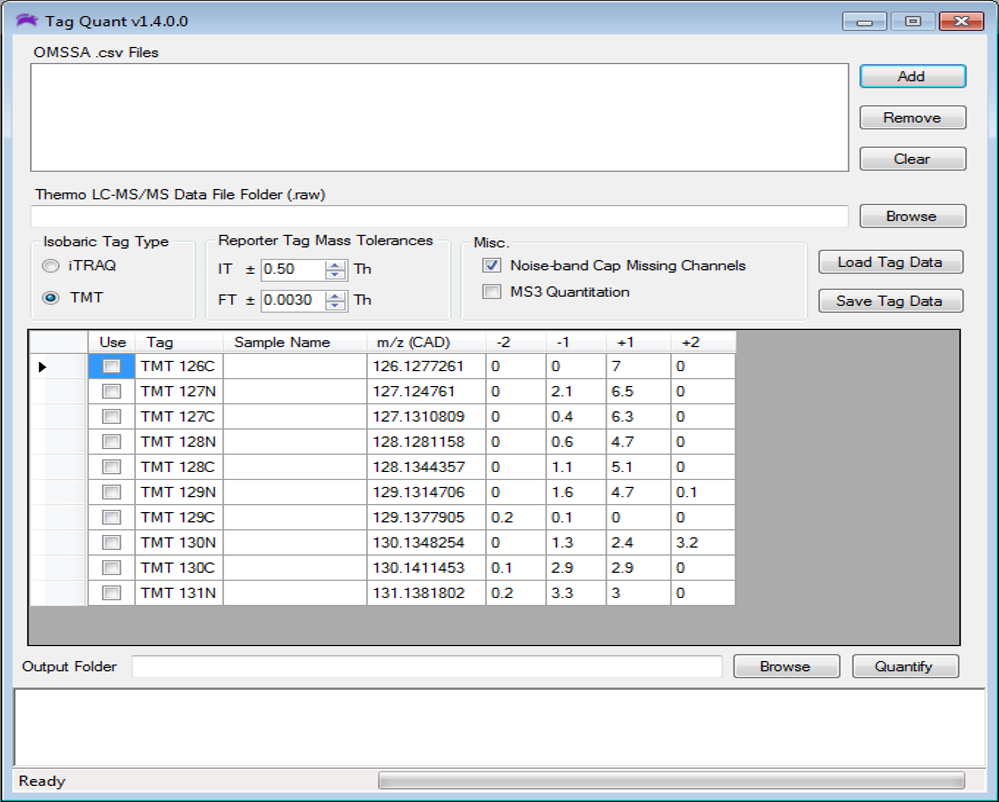
\includegraphics[width=\columnwidth]{csmsl/tagquant.png}
	\mycaption{TagQuant}{The updated GUI for \texttt{TagQuant} allows users to specify the exact labels used and their relative purities. Options for noise-band capping missing channel and quantifying from an MS3 scan are also included.}
	\label{fig:tagquant}
\end{figure}

Numerous improvements have been made to the publication version of \texttt{TaqQuant}. With the advent of high-resolution TMT tags, where two quantiation channels are separated by a very small mass difference (6.32 mDa), additional logic had to be added to handle it.\cite{tmt8,tmt82} Users also started to mix and match channels between different manufacturing lots, resulting in non-standard purity values. This, and other issues, were corrected by providing the user full control over which labels then use to quantify and their respective purities. This change also future proofs the program, allowing it to handle any type of isobaric label later developed without changes to the \texttt{TagQuant} program itself.

Another heavily used feature that was added is noise-band capping missing channels. Sometimes a peak at an expected isobaric tag \mz{} is not present in the MS/MS spectra. Before, this missing value was set to $0$, which would drastically distort the ratio between quantitation channels. In the updated version, \texttt{TagQuant} assigns the missing value to the noise level at the \mz{}. This conservative approach mitigates the distortion of ratios between quantitative channels. An additional feature that was added was enabling quantitation from MS$^3$ spectra. This is the result of purification methods for improving the interference problem of isobaric labels, such as QuantMode and the MS$^3$ methods.\cite{quantmode,ms3}

\subsection*{Protein Hoarder.}
\texttt{Protein Hoarder} infers the most likely proteins identified based on the peptides validated by \texttt{FDR Optimizer} (Figure \ref{fig:hoarder}). The program was initially called \texttt{Protein Herder}, but the program was completely rewritten after publication, and the name was changed to indicate that it is a new program.
\begin{figure}[p]
	\centering
	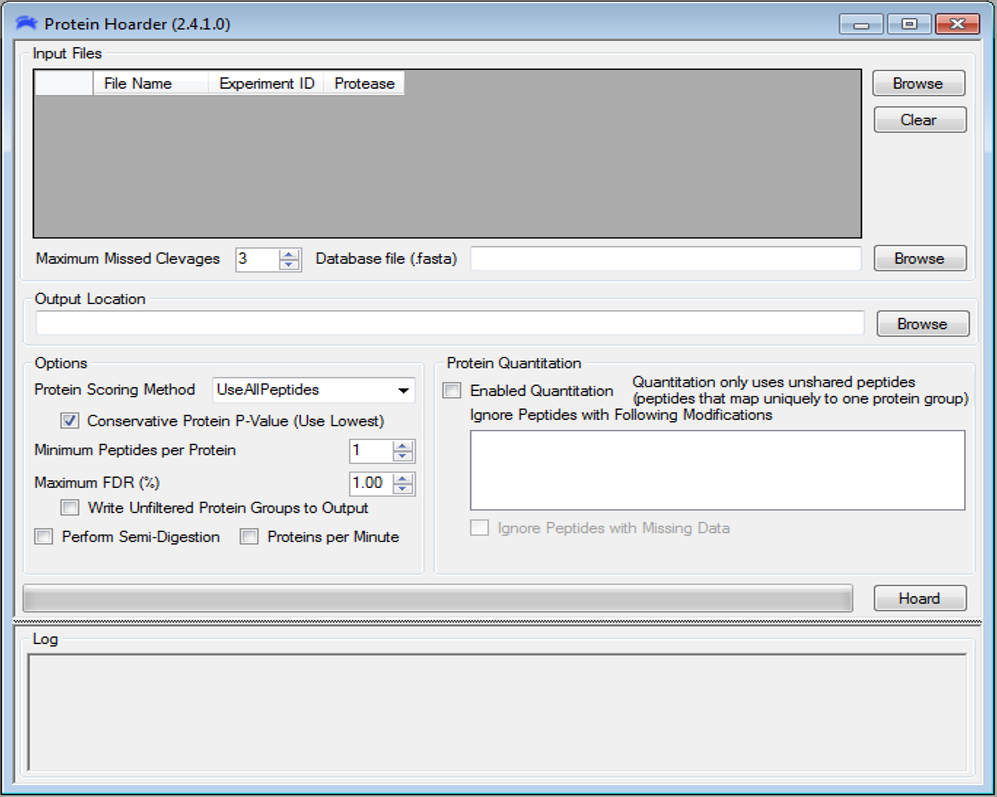
\includegraphics[width=\columnwidth]{csmsl/proteinhoarder.png}
	\mycaption{Protein Hoarder}{The new version of \texttt{Protein Herder} which assembles peptide identifications into protein groups. This version also performs protein quantitation at the same time the protien groups are being assembled.}
	\label{fig:hoarder}
\end{figure}
In this program, peptides are assembled into protein groups based on the law of parsimony, i.e., minimizing the number of protein groups while accounting for all the identified peptides. False discovery analysis is also performed at the protein-level, along with quantitative analysis if requested. The outputs of the program include a \texttt{.csv} file containing all the identified protein groups, along with which peptides are mapped to the groups.

The biggest change between the original and current version is how the peptides are found within the candidate proteins. Previously, each peptide sequence was searched against the whole protein database using brute force. For large databases such as the human proteome, the number of proteins could reach over 150,000 when isoforms and both target and decoy proteins are considered. Even if only 20,000 PSMs were identified, that means 30 billion string comparisons must be made (20,000 x 150,000). This made the original program very slow, and could take up to half a day to assembly protein groups for a human sample. The new algorithm forgoes the string search and uses enzymatic cleavage of the proteins to find the associated peptides. The program preforms an \emph{in silico} digestion of all the proteins and if a generated peptide matches one of the input PSMs, that protein is saved. This process greatly speeds up the whole program, and the same human sample that took half a day to assembly now takes less than 2 minutes. 

Assembled protein groups are further filtered for false discovery using a similar method to \texttt{FDR Optimizer}. Here, the p-value of the protein group (which is the product of all the peptide's e-values for the group) is the ordering metric and the groups are filtered to a specified FDR (e.g., 1\%). In the publication version of \compass{}, there was another program that handled protein quantitation (\texttt{Protein TagQuant}) by summing up all the peptide quantitation for a individual protein group. Here, peptides that are not shared between protein groups (i.e., a unique peptide to the protein group) have their quantitation summed and reported for the protein group. This program was embedded into \texttt{Protein Hoarder} since all the required information for quantitation was already present in the program. This removed the need for using \texttt{Protein TagQuant} altogether, and it was removed from \compass{}. 

\subsection*{LoToR.}
The final program in \compass{} was not present in the initial version. This program is called \texttt{LoToR} (\underline{Lo}calize \underline{To} \underline{R}esidue) and improves the localization of post translational modifications to specific residues on peptides and proteins. Although \texttt{OMSSA}, and other search algorithms, are capable of identifying modification events on peptides, it often does not place the PTM on the correct residue. To address this, \texttt{LoToR} was created to add more rigorous statistical power in localizing PTMs to specific sites. 

\texttt{LoToR} is uses the A-Score algorithm as the primarily metric for assigning statistical confidence.\cite{ascore} In brief, for each PSM that contains a PTM, all possible peptide isoforms are generated. Each of these isoforms represents the unique combination of PTMs applied to every possible site in the peptide. Then each isoform is fragmented and matched to the MS/MS spectrum. After matching, each isoform is compared to every other isoform generated, and the set of fragments that can distinguish them apart are called 'site-determining fragments' (SDFs). The number of identified SDFs for each isoform is then compared, and the two isoforms that have the biggest difference between number of SDFs identified, is declared the best possible isoform. The A-Score for this pair of isoforms is then computed, and if the value is above some defined value (typically 13), it is declared localized.

\section{CSMSL: C\# Mass Spectrometry Library}
Mass spectrometry-based proteomics is a relatively young field that is rapidly evolving, new techniques and technologies are consistently being developed and custom software tools are needed to analyze the data. There are typically three ways to analyze a proteomic dataset: 1) process it through a full-fledged GUI program that has already been developed, 2) manually process the data, or 3) extract data with software tools and analyze in excel. Often a mixture of these three processes are needed to fully analyze a dataset. However, sometimes a complete GUI program is not available for a specific type of data analysis, or, due to the complexity of the data, manual analysis of a dataset in excel or through a spectrum browser (e.g., Thermo XCalibur) is a daunting and time-consuming task. These situations are ideal for a custom analysis program that could facilitate the analysis. Unfortunately, custom programs have shortcomings, 1) not every single researcher knows how to program them and 2) there isn't a free, straightforward programming environment for accessing and manipulating such complex data. The first problem is not easily addressed, but the second one is. There are many tools available for MS analysis on the internet, but most are difficult for novice programmers and are challenging to adapt to a specific need. To fill the gap, I have designed a large proteomic programming library to simplify the data management and manipulation of large-scale proteomic data. It is written for Windows using the .NET Framework V4.0 in the C\# programming language. It is called C\# Mass Spectrometry Library (\csmsl{}) and is freely available at \url{https://github.com/dbaileychess/CSMSL}.

The goals of \csmsl{} is to provide an easy-to-use, powerful, feature-rich library of .NET C\# objects and methods to enable even novice programmers the ability to analyze proteomic data quickly. Simplicity is key, calculating the mass of the peptide sequence 'CSMSL' only requires the following two lines:
\lstset{style=sharpc,numbers=left,numberstyle=\small,keywordstyle=\color{blue},
morekeywords={Peptide,Protein,Console,Protease,ChemicalFormula,List,FastaReader,MSDataFile,MSDataScan}}
\begin{lstlisting}
Peptide peptideA = new Peptide("CSMSL");
Console.WriteLine(peptideA.MonoisotopicMass);
// outputs : 539.20835516707
\end{lstlisting}
In addition to simply syntax, \csmsl{} is designed with performance in mind, allowing even computationally intensive calculations to be completed quickly. For example, a complete yeast database (6,627 proteins) can be loaded from a \texttt{.fasta} file, digested with trypsin (up to 3 missed cleavages, 5 to 35 amino acids in length) in under 2 seconds. If we include the calculation for the [M+H] \mz{} of each of the 913,740 resulting peptides, the total time only goes up to 4 seconds (this includes full chemical formula determination). While \csmsl{} is not expected to meet the performance of advanced compiled languages (e.g., C/C++, Fortran, etc.), its adequate performance plus simplicity of use are sure to be helpful in analyzing data in new and creative ways without significant overhead.

The following sections will succinctly 1) describe the design of the library, 2) show a few example code segments indicating its use, and 3) highlight various features and abilities of the library.

\subsection*{CSMSL Design.}
The \csmsl{} package is divided into three projects. The main project is the library itself (\texttt{CSMSL.csproj}) which contains all the code and objects for data analysis. This project will be described in greater detail in the sections to follow. The other two projects are primary for teaching and development purposes, and will be described here. 

The teaching project is \texttt{CSMSL.Examples.csproj}, which contains short segments of code to show intended use of the library. It is written to aid novice programmers in learning how to program better and how to use the library. It covers a series of example code to demonstrate how to create peptides and proteins, digest proteins, fragment peptides, read in spectral data, among many others. This project is completely separate from \csmsl{} and is only used to demonstrate the features of the main library. 

The development project is \texttt{CSMSL.Tests.csproj}, which hosts all the unit tests for the library. An unit test is a short piece of code that tests one, and only one aspect of the library, hence the term 'unit'. In brief, a short segment of code is written to preform some action (e.g., digest a protein), and the final line contains an assertion statement, declaring that some value needs to possess some trait (e.g., that 5 peptides are produced from a digestion of a certain protein). These assertions can be as simple as an equality ($numOfPeptides == 5$), a comparative condition ($numOfPeptides < 5$), or much more advanced comparisons. Regardless, the point of unit tests is to provide fine grain support and testing for the main project. If any source code is added to the project or a portion of code is changed, all the unit tests report back to the developer if their one piece of functionality is still producing the same result. If not, the developer has a good idea of where the new bug is introduced as only certain unit tests will fail. This helps ensures that new features do not affect other parts of the library or produce unintended bugs. \csmsl{} is heavily tested, especially on the components that are most commonly used.

There also exists a handful of other projects that supply support for third-party tools and access to raw spectral data from different MS vendors. These are located under the \texttt{CSMSL/IO} directory and can be added to a project when needed. The projects that support reading in raw spectral data will be discussed in the features section below. Since \csmsl{} has been developed, it has been heavily incorporated into the source code of \compass{}. This helps simplify every program within \compass{}, as many redundant sections of code was replaced by objects from \csmsl{}. It also helps speed up bug fixes and feature additions, as all programs that use \csmsl{} will benefit from improvements in its code.

\subsection*{CSMSL Examples.}
Functional coding examples are a great way to dive into any programming language/library. \csmsl{} provides a number of example programs, contained within the \texttt{CSMSL.Examples} project, so that people can learn the tools and experiment with different features. Below are a series of examples showing the simplicity and power \csmsl{} offers. All of the examples are written in the C\# language and should be straightforward enough that even non-programmers should be able to follow them.

We will start with the most basic, but most commonly used features: proteins and peptides. The following code first constructs a new peptide object in memory, labels it as '\texttt{peptideA}' and then prints its monoisotopic mass to the console window.
\begin{lstlisting}
Peptide peptideA = new Peptide("FLTTSNALKEN");
Console.Write(peptideA.MonoisotopicMass);
// outputs: 1236.635016661
\end{lstlisting}
Of course there are a plethora of tools and websites that could calculate the monoisotopic mass of a peptide sequence, the novel aspect is its simplicity and the ability to programmatically control it. 

Peptides and proteins can be modified post transitionally and \csmsl{} enables easy methods for modifying peptides. Taking the previous example further, to modified the serine residue ('S') with a phosphorylation is easy:
\begin{lstlisting}
Peptide peptideA = new Peptide("FLTTSNALKEN");
ChemicalFormula phospho = new ChemicalFormula("HPO3");
peptideA.SetModification(phospho, 'S');
Console.Write(peptideA.MonoisotopicMass);
// outputs: 1316.60134718175
\end{lstlisting}
Only two new lines are inserted. Line 2 creates the phosphorylation modification (labeled as '\texttt{phospho}'), and introduces another \csmsl{} object called \texttt{ChemicalFormula}, which represents a chemical structure. The third line sets the '\texttt{phospho}' chemical formula to modified all serine residues in \texttt{peptideA}. Since there is only one serine in \texttt{peptideA}, the resulting mass is $1316.601347$ and the difference is $79.96637$, which corresponds exactly to the mass of an phosphorylation.

Another important feature often used is protein digestion. In nature, peptides often arise from the proteolyic digestion of intact proteins by proteases, such as trypsin. \csmsl{} can do the same thing done in a test tube but \emph{in silico}. Below is an example of a tryptic digestion of a single protein. It produces a list of \texttt{Peptide} objects which are then printed to the screen.
\begin{lstlisting}
Protein proteinA = new Protein("MMGFKQLITTGSSSRSSSSKDTSST");
List<Peptide> peptides = proteinA.Digest(Protease.Trypsin);
Console.Write(peptides);
// outputs: MMGFK, QLITTGSSS, SSSSK, etc...
\end{lstlisting}
The first line creates a new \texttt{protein} object in memory, just like the peptide example above. The second line takes the created protein (\texttt{proteinA}) and performs a digestion with trypsin. The result (the left hand side of the equation) is a list of \texttt{Peptide} objects. The final line then takes all those peptide sequences and prints them to the screen. This is a simple digestion, but there exists many more options, such as maximum and minimum peptide length, max missed cleavages, partial digestion, etc. All these options will not be explored here, but almost anything you could do on a physical protein/peptide, can be performed \emph{in silico} using \csmsl{}.

\subsection*{Full Proteome Tryptic Digestion Example.} The code section shows a complete example of a tryptic digestion of a yeast proteoeme. Its inclusion here is to demonstrate that a fairly complicated task can be perform with only a few lines of code that should be easily understandable to a novice programmer.
\begin{lstlisting}
using (FastaReader reader = new FastaReader("yeast.fasta"))
{
 Protease trypsin = Proteases.Trypsin;
 int max = 3;  // Maximum number of missed cleavages
 foreach (Protein protein in reader.ReadNextProtein())
 {
  foreach (Peptide peptide in protein.Digest(trypsin, max))
  {
    Console.WriteLine(peptide.MonoisotopicMass);  
  }
 }
}       
\end{lstlisting}
Line 1 opens up a connection to a protein database file named ''yeast.fasta'' located on the computer. The \texttt{FastaReader} object provides methods for reading and accessing proteins contained in a fasta-formatted file. The third line sets up a variable that represents the typsin protease. Line 4 sets another variable defining the maximum number of missed cleavages allowed for the digestion. The fifth line iterates over each \texttt{Protein} within the fasta file, by calling the 'ReadNextProtein()' method. The lines 6 through 11 are then performed for each protein read in by line 5. Line 7 iterates over every peptide generated from the digestion of the protein by trypsin and a maximum missed cleavage of three. Again, lines 8 through 10 are repeated for every generated peptide. The last important line is line 9, where the produced peptide's monoisotopic mass is written to the console window on the computer. In only 12 lines of code, a complicated task is accomplished using \csmsl{} objects and methods. Similarly, other proteomic analysis and computations can be expedient coded and perform. These examples can be found in more details in the \texttt{CSMSL.Examples.csproj} project file.

\subsection*{CSMSL Features and Objects.}
The \csmsl{} library has too many features to be listed in full, so only a few of the most important features will be highlighted here. Since this is primarily a proteomic library, we will start off with proteins and chemicals and then transition to spectral classes. 

Starting from the smallest object and growing bigger, elemental isotopes represent the basic building block of everything else that has mass. Each isotope has a few intrinsic properties, most important are mass and the element it belongs to. A single element may contain a set of different isotopes (e.g., $^{12}C$, $^{13}C$, and $^{14}C$), and the most naturally-abundant isotope is declared the principal isotope of the element. Thus elements and their most abundant isotopes are interchangeable with each other (i.e., $^{12}C$ and $C$ refer to the same object). When other isotopes are needed, you need to specify which isotope you want to use (e.g., $C\{13\}$ mean you want $^{13}C$ instead of $^{12}C$). This feature is important because stable isotope quantitative labeling is a very common analysis, and we wanted to design the library with it in mind. All the elements, and thus isotopes, are assembled into the periodic table of elements for easy access.

In \csmsl{}, chemical formulas are represented as a set of isotopes without any spatial connectivity. Keeping the three dimensional structure of molecules is not an important aspect of most proteomic work, and we purposefully left this out in favor of speed and memory savings. Additionally, a chemical formula generator is available to list all possible chemical formulas given an exact mass. Such features are used in indentifying unknown peaks in high-resolution mass spectra. The mass of a chemical formula is the simple summation of all of its isotopes. Almost every other object in this library is a chemical formula (e.g., proteins, peptides, amino acids, modifications, etc.)  with additional properties of its own. Amino acids are simply a chemical formula with character symbol to represent which one it is. The 20 common amino acids are prebuilt by the library and ready to use, but custom amino acids can be added easily.

Probably the most important classes in the library are the protein and peptide classes. Since both a protein and peptide can be thought of as a string of amino acids, both classes are modeled off a single base class called \texttt{AminoAcidPolymer}. This class can just be thought of as an fancy array of amino acids, spanning from the N-terminus to the C-terminus. Each location on this array (i.e., amino acids or termini) can be modified by a chemical formula. The mass of the \texttt{AminoAcidPolymer} is again the simple summation of all its amino acids and modifications. Peptides have special methods for producing fragments ions (e.g., a, b, c, x, y, z-type), as well as others. Fragment ions again are just chemical formulas, but they keep track of what amino acids and modifications are contain in each fragment. This is particularly useful when matching fragment ions against a mass spectrum, as it fully annotates the spectra during the matching steps. Proteins have methods for proteolytic digestion by any enzyme. Users can also define their own proteases to use, and they will be compatible with all the features of digestion (e.g., missed cleavages, min/max lengths, semi-digestions, etc.).

Finally, a set of spectral-related classes are included to provide easy access to spectral data. In \csmsl{} spectra are comprised of a ordered list of \texttt{Peaks}, which represents the \mz{} and intensity of the peak. These \texttt{Peaks} objects can be extended to contain additional information (e.g., charge, noise, baseline intensity, etc.) provided by the instrument. The class \texttt{Spectrum} contains the data of a specific spectrum and provides a series of methods for easy data access. Since a large part of proteomic analysis is looking for peaks within a spectra, probably the most important method is the \texttt{GetClosestPeak()} method. This uses a binary-search algorithm to quickly find the closest peak to a given \mz{} value, and this operation takes on average $O(\log N)$ time, where $N$ is the number of peaks in the spectra. Even with complex spectra of 1,000 peaks, it only takes about 7 comparisons to locate a peak.

\subsection*{Spectral Data Access.}
Perhaps the most useful feature \csmsl{} provides is access to raw spectral data collected by the MS. Instrument vendors usually offer an application programming interface (API) for accessing data from their propriety data formats (e.g., \texttt{.raw} for Thermo, \texttt{.d} for Agilent, etc.). While it is possible to use them on own, a few factors make them difficult to implement. First, they are geared to more advanced programmers and often have incomplete documentation. This makes learning how to access the data difficult, even for good programmers. For people who don't know how to program at all, it would be very difficult to understand and make work. Secondly, each instrument vendor creates their own API which is incompatible with everyone else. Thus if you desire to analyze two different types of data with your program, you'll have to use both APIs to achieve the same result. This can often lead to bugs and frustration. Lastly, you have to be an expert in each API in order to fully use their capabilities. \csmsl{} solves these issues by having a single and simple interface to accessing the data. No matter where the data was produced, the same code can access the underlying data, without the users having to fiddle around. 

The following example shows how to read in every MS spectra from a \texttt{.raw} file generated from a Thermo mass spectrometer.
\begin{lstlisting}
MSDataFile dataFile = new ThermoRawFile("somerawfile.raw")
dataFile.Open();                   
foreach (MSDataScan scan in dataFile)
{             
    Console.WriteLine('Number of Peaks: '+scan.PeakCount);
}
\\ outputs:
\\   Number of Peaks: 1052
\\   Number of Peaks: 523
\\   etc..
\end{lstlisting}
First, in line 1 a mass spectrum data file is constructed from a file on the computer, named ''somerawfile.raw''. The second line opens a connection to the file, and the third line iterates over each MS scan within that file. The number of peaks contained within that scan is then printed to the screen. The beauty of this example is that the first line could be changed to:
\begin{lstlisting}
//MSDataFile dataFile = new ThermoRawFile("somerawfile.raw")
MSDataFile dataFile = new AgilentDDirectory("somerawfile.d")
\end{lstlisting}
and the program would continue to work, even though it is now accessing MS data collected by an Agilent mass spectrometer. Having this sort of flexibility built in from the start enables programmers to program their tools once and have it work with data from any source supported. As of this publication, only Thermo \texttt{.raw}, Agilent \texttt{.d} and \texttt{.mzML} formats are supported. However, other vendors could be added in in the future without breaking code. While there are too many features to be fully explained here, the concept of a simple and consistent way to access spectral data is a key component of \csmsl{}. 

\bibliographystyle{ieeetr}
\bibliography{csmsl}
\chapter{The Future of Intelligent Data Acquisition Methods}

The work presented here is on the forefront of mass spectrometry based acquisition methods. 

There are two main methods for increasing the intelligence of mass spectrometers. The first would be if there is a home built mass spectrometer that is controlled by custom controllers and software. The other way is to modify and extend commercially available mass spectrometers with the desired abilities. For large scale proteomic work, the former approach is not straightforward, as a vast majority of large-scale publication use commercial instruments for data acquisition. Custom built mass spectrometers often focus on a very specific task (e.g., new mass analyzer, new dissociation technique, etc.) and rarely are geared for high-performance, large-scale protein experiments. Commercial instruments, on the other hand, are primarily developed to take the best technologies available and combine them into one unified package. This results in a powerful and stable instrument that can handle the largest experiments. However, in order to protect their intellectual property, instrument vendors are usually highly restrictive in how their instruments are used. This makes implementing novel acquisition methods very difficult, and therefore general acceptance of new methods is slow. Thus, the most important factor in the future of intelligent data acquisition methods is increasing the accessibility and availability.

\section{Accessibility of Intelligent Mass Spectrometers}
Probably the best way to propel the development of intelligent acquisition methods forward is to increase its accessibility and availability to researchers. This is challenging since instrument vendors are highly protective of their products; they have to protect their intellectual property and public imagine while providing state-of-the-art technologies to consumers. They cannot release access to their control logic in fears of competitors gaining an edge. They also worry that supporting third-party programs for their instruments could damage their reputation. Our lab, which has developed multiple technologies now commercialized, know first hand the care instrument vendors take in releasing third-party technologies to the general consumer. 




\section*{Need}
Behind any feature or tool, there always lies the question ''Is this needed?'' Can some other method provide benefits 


\section*{title}


%% Do you have appendices?  If so, add them here, just like chapters.
% \begin{appendices}
% \include{backmatter/appendix1}
% \end{appendices}

%% Are you a big nerd with a colophon?  Add it here.
\begin{colophon}
This template uses Gyre Pagella by default.  (I used Arno Pro in my dissertation.)

Feel free to give me a shout-out in your colophon or acks if this template is useful for you.  Good luck!

\end{colophon}

%% Want an index?  Neither did I.
%\printindex

\end{document}
